% Options for packages loaded elsewhere
% Options for packages loaded elsewhere
\PassOptionsToPackage{unicode}{hyperref}
\PassOptionsToPackage{hyphens}{url}
\PassOptionsToPackage{dvipsnames,svgnames,x11names}{xcolor}
%
\documentclass[
  english,
  10pt,
  letterpaper,
  DIV=11,
  numbers=noendperiod]{scrartcl}
\usepackage{xcolor}
\usepackage[margin=1in]{geometry}
\usepackage{amsmath,amssymb}
\setcounter{secnumdepth}{5}
\usepackage{iftex}
\ifPDFTeX
  \usepackage[T1]{fontenc}
  \usepackage[utf8]{inputenc}
  \usepackage{textcomp} % provide euro and other symbols
\else % if luatex or xetex
  \usepackage{unicode-math} % this also loads fontspec
  \defaultfontfeatures{Scale=MatchLowercase}
  \defaultfontfeatures[\rmfamily]{Ligatures=TeX,Scale=1}
\fi
\usepackage{lmodern}
\ifPDFTeX\else
  % xetex/luatex font selection
\fi
% Use upquote if available, for straight quotes in verbatim environments
\IfFileExists{upquote.sty}{\usepackage{upquote}}{}
\IfFileExists{microtype.sty}{% use microtype if available
  \usepackage[]{microtype}
  \UseMicrotypeSet[protrusion]{basicmath} % disable protrusion for tt fonts
}{}
\makeatletter
\@ifundefined{KOMAClassName}{% if non-KOMA class
  \IfFileExists{parskip.sty}{%
    \usepackage{parskip}
  }{% else
    \setlength{\parindent}{0pt}
    \setlength{\parskip}{6pt plus 2pt minus 1pt}}
}{% if KOMA class
  \KOMAoptions{parskip=half}}
\makeatother
% Make \paragraph and \subparagraph free-standing
\makeatletter
\ifx\paragraph\undefined\else
  \let\oldparagraph\paragraph
  \renewcommand{\paragraph}{
    \@ifstar
      \xxxParagraphStar
      \xxxParagraphNoStar
  }
  \newcommand{\xxxParagraphStar}[1]{\oldparagraph*{#1}\mbox{}}
  \newcommand{\xxxParagraphNoStar}[1]{\oldparagraph{#1}\mbox{}}
\fi
\ifx\subparagraph\undefined\else
  \let\oldsubparagraph\subparagraph
  \renewcommand{\subparagraph}{
    \@ifstar
      \xxxSubParagraphStar
      \xxxSubParagraphNoStar
  }
  \newcommand{\xxxSubParagraphStar}[1]{\oldsubparagraph*{#1}\mbox{}}
  \newcommand{\xxxSubParagraphNoStar}[1]{\oldsubparagraph{#1}\mbox{}}
\fi
\makeatother


\usepackage{longtable,booktabs,array}
\newcounter{none} % for unnumbered tables
\usepackage{calc} % for calculating minipage widths
% Correct order of tables after \paragraph or \subparagraph
\usepackage{etoolbox}
\makeatletter
\patchcmd\longtable{\par}{\if@noskipsec\mbox{}\fi\par}{}{}
\makeatother
% Allow footnotes in longtable head/foot
\IfFileExists{footnotehyper.sty}{\usepackage{footnotehyper}}{\usepackage{footnote}}
\makesavenoteenv{longtable}
\usepackage{graphicx}
\makeatletter
\newsavebox\pandoc@box
\newcommand*\pandocbounded[1]{% scales image to fit in text height/width
  \sbox\pandoc@box{#1}%
  \Gscale@div\@tempa{\textheight}{\dimexpr\ht\pandoc@box+\dp\pandoc@box\relax}%
  \Gscale@div\@tempb{\linewidth}{\wd\pandoc@box}%
  \ifdim\@tempb\p@<\@tempa\p@\let\@tempa\@tempb\fi% select the smaller of both
  \ifdim\@tempa\p@<\p@\scalebox{\@tempa}{\usebox\pandoc@box}%
  \else\usebox{\pandoc@box}%
  \fi%
}
% Set default figure placement to htbp
\def\fps@figure{htbp}
\makeatother


% definitions for citeproc citations
\NewDocumentCommand\citeproctext{}{}
\NewDocumentCommand\citeproc{mm}{%
  \begingroup\def\citeproctext{#2}\cite{#1}\endgroup}
\makeatletter
 % allow citations to break across lines
 \let\@cite@ofmt\@firstofone
 % avoid brackets around text for \cite:
 \def\@biblabel#1{}
 \def\@cite#1#2{{#1\if@tempswa , #2\fi}}
\makeatother
\newlength{\cslhangindent}
\setlength{\cslhangindent}{1.5em}
\newlength{\csllabelwidth}
\setlength{\csllabelwidth}{3em}
\newenvironment{CSLReferences}[2] % #1 hanging-indent, #2 entry-spacing
 {\begin{list}{}{%
  \setlength{\itemindent}{0pt}
  \setlength{\leftmargin}{0pt}
  \setlength{\parsep}{0pt}
  % turn on hanging indent if param 1 is 1
  \ifodd #1
   \setlength{\leftmargin}{\cslhangindent}
   \setlength{\itemindent}{-1\cslhangindent}
  \fi
  % set entry spacing
  \setlength{\itemsep}{#2\baselineskip}}}
 {\end{list}}
\usepackage{calc}
\newcommand{\CSLBlock}[1]{\hfill\break\parbox[t]{\linewidth}{\strut\ignorespaces#1\strut}}
\newcommand{\CSLLeftMargin}[1]{\parbox[t]{\csllabelwidth}{\strut#1\strut}}
\newcommand{\CSLRightInline}[1]{\parbox[t]{\linewidth - \csllabelwidth}{\strut#1\strut}}
\newcommand{\CSLIndent}[1]{\hspace{\cslhangindent}#1}

\ifLuaTeX
\usepackage[bidi=basic,shorthands=off]{babel}
\else
\usepackage[bidi=default,shorthands=off]{babel}
\fi
\ifLuaTeX
  \usepackage{selnolig} % disable illegal ligatures
\fi


\setlength{\emergencystretch}{3em} % prevent overfull lines

\providecommand{\tightlist}{%
  \setlength{\itemsep}{0pt}\setlength{\parskip}{0pt}}



 


\KOMAoption{captions}{tableheading}
\makeatletter
\@ifpackageloaded{caption}{}{\usepackage{caption}}
\AtBeginDocument{%
\ifdefined\contentsname
  \renewcommand*\contentsname{Table of contents}
\else
  \newcommand\contentsname{Table of contents}
\fi
\ifdefined\listfigurename
  \renewcommand*\listfigurename{List of Figures}
\else
  \newcommand\listfigurename{List of Figures}
\fi
\ifdefined\listtablename
  \renewcommand*\listtablename{List of Tables}
\else
  \newcommand\listtablename{List of Tables}
\fi
\ifdefined\figurename
  \renewcommand*\figurename{Figure}
\else
  \newcommand\figurename{Figure}
\fi
\ifdefined\tablename
  \renewcommand*\tablename{Table}
\else
  \newcommand\tablename{Table}
\fi
}
\@ifpackageloaded{float}{}{\usepackage{float}}
\floatstyle{ruled}
\@ifundefined{c@chapter}{\newfloat{codelisting}{h}{lop}}{\newfloat{codelisting}{h}{lop}[chapter]}
\floatname{codelisting}{Listing}
\newcommand*\listoflistings{\listof{codelisting}{List of Listings}}
\usepackage{amsthm}
\theoremstyle{definition}
\newtheorem{definition}{Definition}[section]
\theoremstyle{plain}
\newtheorem{theorem}{Theorem}[section]
\theoremstyle{plain}
\newtheorem{lemma}{Lemma}[section]
\theoremstyle{remark}
\AtBeginDocument{\renewcommand*{\proofname}{Proof}}
\newtheorem*{remark}{Remark}
\newtheorem*{solution}{Solution}
\newtheorem{refremark}{Remark}[section]
\newtheorem{refsolution}{Solution}[section]
\makeatother
\makeatletter
\makeatother
\makeatletter
\@ifpackageloaded{caption}{}{\usepackage{caption}}
\@ifpackageloaded{subcaption}{}{\usepackage{subcaption}}
\makeatother
\usepackage{bookmark}
\IfFileExists{xurl.sty}{\usepackage{xurl}}{} % add URL line breaks if available
\urlstyle{same}
\hypersetup{
  pdftitle={One-Phase Euler Coordinates for Affine Brownian Factors},
  pdfauthor={Complex--Itô Random-Walk Research Project},
  pdflang={en},
  pdfkeywords={affine Brownian motion, Bachelier model, stochastic
coordinate transformation, Euler form, arctangent
compactification, transition density, option Greeks, stochastic
dimension, logarithmic spiral, geometric numerical integration},
  colorlinks=true,
  linkcolor={blue},
  filecolor={Maroon},
  citecolor={Blue},
  urlcolor={Blue},
  pdfcreator={LaTeX via pandoc}}


\title{One-Phase Euler Coordinates for Affine Brownian Factors}
\usepackage{etoolbox}
\makeatletter
\providecommand{\subtitle}[1]{% add subtitle to \maketitle
  \apptocmd{\@title}{\par {\large #1 \par}}{}{}
}
\makeatother
\subtitle{Exact classification, phase diffusion, and conjugate
normal-model pricing}
\author{Complex--Itô Random-Walk Research Project}
\date{July 25, 2026}
\begin{document}
\maketitle
\begin{abstract}
We classify the nondegenerate affine complex Brownian processes
\(Z_t=Z_0+at+bW_t\) that admit an exact, lossless, time-independent
Euler representation \(Z_t=Z_0r(\theta_t)e^{i\theta_t}\) in which the
genuine polar phase \(\theta_t\) is the only stochastic state
coordinate. For \(Z_0b\ne0\), such a representation exists if and only
if \(a/b\in\mathbb R\) and \(b/Z_0\notin\mathbb R\). The first condition
fixes all temporal supports to one affine line; the second makes its
argument injective by requiring that line to miss the polar origin.
Writing \(a=\lambda b\) and \(b/Z_0=\rho e^{i\phi}\), the representation
and inverse are \(r(\theta)=\sin\phi/\sin(\phi-\theta)\) and
\(x(\theta)=\sin\theta/[\rho\sin(\phi-\theta)]\) on a unique open phase
interval of length \(\pi\). The canonical financial chart is
\(1+iX_t/c=\sec\theta_t e^{i\theta_t}\) with
\(\theta_t=\arctan(X_t/c)\). We derive its Itô and Stratonovich
equations, generator, exact transition kernel, natural boundaries, and
transported additive group. A rigidity result shows that
constant-coefficient additive dynamics force a line, whereas compatible
multiplicative dynamics force a logarithmic spiral. Under a pricing
measure, the chart conjugates the Bachelier generator, option values,
Greeks, and hedges without changing the financial model. Reproducible
experiments verify reconstruction, strong convergence, transition and
pricing PDEs, and exact Bachelier prices and Greeks. Matched controls
show that the chart creates neither an additional stochastic dimension
nor automatic Monte Carlo variance reduction, holomorphic structure,
path compression, or universal numerical acceleration. The result is
therefore an exact geometric coordinate and a classification theorem,
not a replacement for Itô calculus or a new pricing model.
\end{abstract}

\renewcommand*\contentsname{Table of contents}
{
\setcounter{tocdepth}{2}
\tableofcontents
}

\textbf{Mathematics Subject Classification (2020):} 60H10, 60J60, 91G20,
91G60, 65C30.

\textbf{JEL classification:} C02, C63, G12, G13.

\section{Introduction}\label{sec-introduction}

Euler's identity

\[
e^{i\theta}=\cos\theta+i\sin\theta
\]

turns phase into planar rotation, while the Itô table records the
quadratic variation of Brownian motion through \(d[W,W]_t=dt\). Their
superficial resemblance---each contains a consequential square---often
motivates an attempt to combine drift and Brownian noise into one
complex exponential. The motivation is geometrically natural, but the
two squares have different meanings. The identity \(i^2=-1\) is
algebraic. Brownian quadratic variation is a limiting path property. A
valid bridge between them must pass through Itô's formula, support
geometry, and an invertible state map.

This paper asks a precise version of that question. Given a real
standard Brownian motion \(W\) and

\begin{equation}\protect\phantomsection\label{eq-affine-process}{
Z_t=Z_0+at+bW_t,\qquad Z_0,a,b\in\mathbb C,
}\end{equation}

when can the complete process be written

\begin{equation}\protect\phantomsection\label{eq-requested-form}{
Z_t=Z_0r(\theta_t)e^{i\theta_t}
}\end{equation}

with a deterministic, time-independent radius \(r\) and one real
stochastic phase \(\theta\) that is both the genuine polar argument and
a lossless state coordinate? The requirement is substantially stronger
than merely encoding a real variable by some measurable real number. It
asks the polar angle itself to carry the random state while the modulus
is a deterministic function of that angle.

The central result is an exact classification. In the nondegenerate case
\(Z_0b\ne0\), Eq.~\ref{eq-requested-form} exists if and only if

\begin{equation}\protect\phantomsection\label{eq-classification-preview}{
\boxed{
\frac{a}{b}\in\mathbb R,
\qquad
\frac{b}{Z_0}\notin\mathbb R.
}
}\end{equation}

The first condition says that drift and diffusion are real-collinear, so
all fixed-time supports coincide with one affine line. The second says
that the line misses the origin, making its continuous argument strictly
monotone. If

\[
a=\lambda b,\qquad
\frac b{Z_0}=\rho e^{i\phi},\qquad
x_t=\lambda t+W_t,
\]

then the exact formula is

\begin{equation}\protect\phantomsection\label{eq-general-preview}{
\boxed{
Z_t
=
Z_0\frac{\sin\phi}{\sin(\phi-\theta_t)}e^{i\theta_t},
\qquad
\theta_t=\arg\!\left(1+\rho e^{i\phi}x_t\right).
}
}\end{equation}

The inverse is explicit and the admissible phase interval has length
\(\pi\). Thus an additive affine process can acquire a genuine, lossless
stochastic phase, but it cannot execute unrestricted winding.

The canonical form is especially transparent. For an arithmetic Brownian
factor \(X\) and scale \(c>0\),

\begin{equation}\protect\phantomsection\label{eq-canonical-preview}{
\boxed{
1+i\frac{X_t}{c}
=\sec\theta_t\,e^{i\theta_t},
\qquad
\theta_t=\arctan\!\left(\frac{X_t}{c}\right),
\qquad
X_t=c\tan\theta_t.
}
}\end{equation}

The state formula contains one stochastic variable, \(\theta_t\). Time
still indexes the process and Brownian randomness still drives its law;
neither can be removed from a nontrivial stochastic model. The point is
state factorization, not the disappearance of stochasticity.

\begin{figure}[tbp]

\centering{

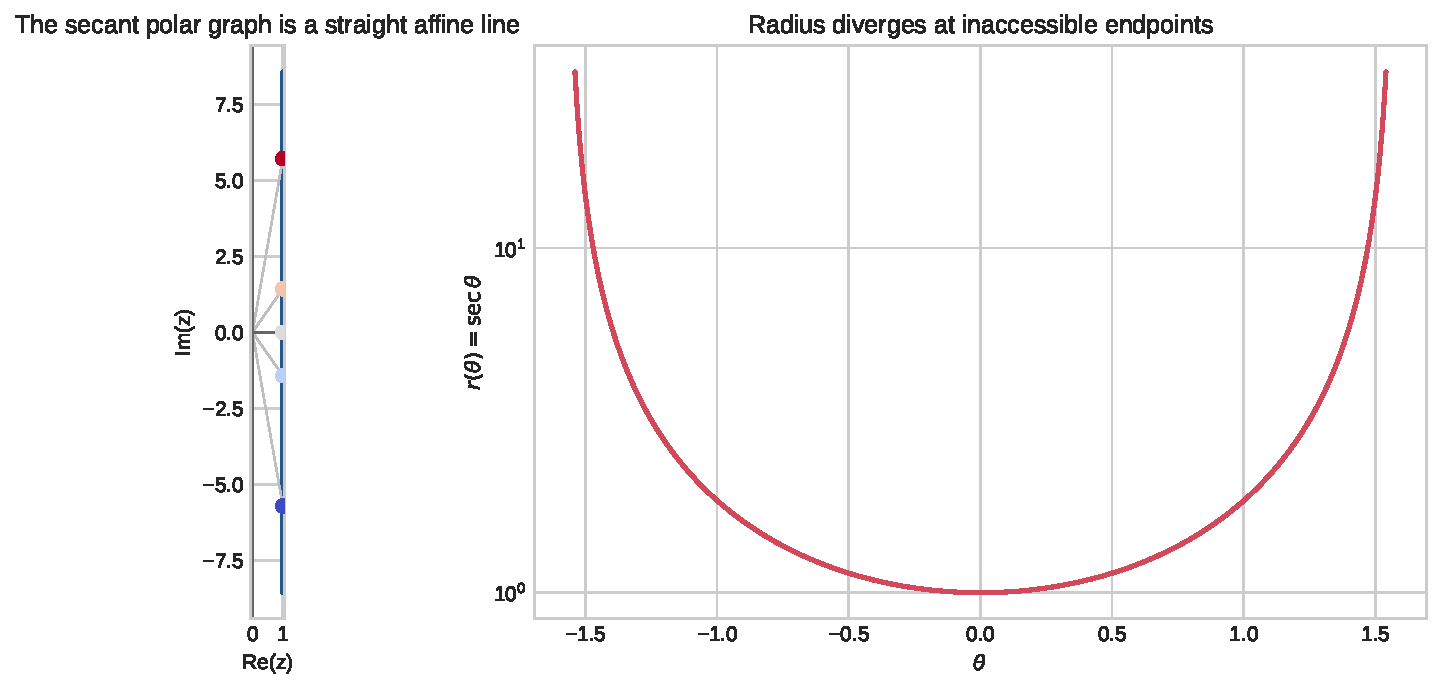
\includegraphics[width=1\linewidth,height=\textheight,keepaspectratio,alt={Left: the secant Euler curve lies on a vertical affine line and selected radius vectors point to it. Right: secant radius versus phase on an open half-turn, diverging near both endpoints.}]{figures/vector/f01_secant_geometry.pdf}

}

\caption{\label{fig-secant-geometry}The canonical secant polar graph,
its affine-line image, and the radius divergence at the inaccessible
phase endpoints.}

\end{figure}%

Figure~\ref{fig-secant-geometry} reveals the principal geometric fact.
Although \(\sec\theta\) and \(e^{i\theta}\) look radial and rotational
separately, their product is

\[
\sec\theta e^{i\theta}=1+i\tan\theta,
\]

a straight line. The representation changes coordinates and traversal
speed; it does not turn rank-one additive Brownian motion into planar
Brownian motion.

\subsection{Contributions}\label{contributions}

The paper makes five contributions.

\begin{enumerate}
\def\labelenumi{\arabic{enumi}.}
\tightlist
\item
  It distinguishes measurable scalar factorization from a genuine,
  continuous, lossless Euler phase and proves the complete affine
  classification Eq.~\ref{eq-classification-preview}, including a
  randomized-time necessity argument that respects almost-sure
  quantifiers.
\item
  It derives the general phase radius, inverse, domain, Itô and
  Stratonovich dynamics, generator, transition density, semigroup, exact
  step, and boundary classification.
\item
  It proves a local rigidity dictionary: constant additive complex noise
  forces a straight line, whereas compatible constant multiplicative
  noise forces a logarithmic spiral. It also identifies the transported
  group law of the phase chart.
\item
  It develops a financial interpretation in which the complex state is
  an auxiliary coordinate for a real Bachelier factor. Pricing, Greeks,
  hedging, and the pricing PDE are conjugate under the chart.
\item
  It subjects every broad implication to matched numerical controls.
  Those controls separate exact coordinate benefits from unsupported
  claims of added dimension, winding, variance reduction, path
  compression, holomorphic calculus, or universal acceleration.
\end{enumerate}

The arctangent transform, stochastic changes of variables, Bachelier
pricing, compactification of unbounded domains, stochastic exponentials,
and complex linear SDEs are established subjects. The contribution is
the classification and the integrated stochastic-financial analysis, not
the invention of those ingredients.

\subsection{Organization}\label{organization}

Section~\ref{sec-literature} positions the result.
Section~\ref{sec-setup} fixes the probability, geometric, and financial
assumptions. Section~\ref{sec-factorization} isolates measurable
factorization and support geometry. Section~\ref{sec-classification}
proves the affine theorem and handles exceptional cases.
Section~\ref{sec-canonical} develops the canonical secant chart,
followed by its stochastic theory in Section~\ref{sec-phase-theory}.
Section~\ref{sec-rigidity} compares additive lines, multiplicative
spirals, and transported groups. Section~\ref{sec-finance} establishes
pricing conjugacy and Section~\ref{sec-numerics} reports the
reproducible evidence. Section~\ref{sec-vector} and
Section~\ref{sec-complex-analysis} delimit the vector and
complex-analytic implications. Section~\ref{sec-research-agenda} gives
qualified applications and open problems. Technical derivations and
reproducibility details appear in the appendices.

\section{Literature and novelty boundary}\label{sec-literature}

\subsection{Brownian motion, random walks, and
finance}\label{brownian-motion-random-walks-and-finance}

Bachelier's 1900 dissertation introduced a Gaussian diffusion model for
speculative prices and an early option-pricing calculation (Bachelier
1900). Wiener's path-space construction provided a mathematical
foundation for Brownian motion (Wiener 1923), and Donsker's invariance
principle later made the random-walk-to-Brownian limit precise (Donsker
1951). Modern Brownian-motion treatments supply the support, path, and
quadratic-variation facts used below (Mörters and Peres 2010). We do not
retroactively attribute modern semimartingale or risk-neutral machinery
to Bachelier; those frameworks came later.

Itô's foundational papers introduced stochastic integration and the
second-order change-of-variables rule (Itô 1944, 1951). Girsanov
established absolutely continuous measure changes for diffusion
processes (Girsanov 1960), and Kac connected Wiener functionals to
parabolic equations (Kac 1949). Modern derivative valuation rests on
no-arbitrage, replication, and martingale arguments developed in
particular by Black and Scholes, Merton, and Harrison and Pliska (Black
and Scholes 1973; Merton 1973; Harrison and Pliska 1981).

\subsection{Transformations and angular
coordinates}\label{transformations-and-angular-coordinates}

Nonlinear diffusion coordinates are classical. Lamperti transformations
normalize scalar diffusion coefficients (Lamperti 1964). Doss and
Sussmann relate suitable stochastic equations to pathwise ordinary
equations (Doss 1977; Sussmann 1977), while Zvonkin uses a one-to-one
phase-space transformation to remove irregular drift (Zvonkin 1974).
Särkkä and Solin use an arctangent transform of Brownian motion as an
exact nonlinear-SDE benchmark (Särkkä and Solin 2019). These works rule
out any novelty claim for applying \(\arctan\) or Itô's formula to a
scalar diffusion.

Projecting a Gaussian vector onto an angle is also established in
directional statistics (Pukkila and Rao 1988; Wang and Gelfand 2013).
The law studied here is different from a generic projected bivariate
normal: its Gaussian support is one affine line, and its phase density
follows from a one-dimensional monotone change of variables.

Genuine planar Brownian winding requires two-dimensional motion and has
asymptotic behavior absent from a one-line process (Spitzer 1958; Pitman
and Yor 1986). Stereographic projection of Brownian motion likewise has
a substantial prior theory (Carne 1985). Those literatures are
comparisons, not derivations of the present phase.

\subsection{Multiplicative and complex stochastic
models}\label{multiplicative-and-complex-stochastic-models}

Stochastic exponentials and logarithms are part of established
semimartingale calculus (Doléans-Dade 1970; Larsson and Ruf 2019).
Modern representation and multiplicative-compensation frameworks further
systematize this theory (Černý and Ruf 2022, 2023). Complex scalar
linear equations and complex geometric Brownian motion appear explicitly
in numerical-stability research (Buckwar et al. 2006; Perret 2010).
Accordingly, the logarithmic-spiral comparator derived below is not a
new complex GBM. Its role is to expose why unbounded lossless winding is
compatible with multiplicative, but not additive, constant-coefficient
dynamics.

\subsection{Financial and computational
precedents}\label{financial-and-computational-precedents}

The normal model remains relevant when negative forwards or strikes are
plausible. Schachermayer and Teichmann compare Bachelier and
Black--Merton--Scholes asymptotics (Schachermayer and Teichmann 2008),
while Choi et al.~survey normal-model pricing, volatility conversion,
and risk management (Choi et al. 2022). CME's 2020 clearing advisory
documents a practical switch to Bachelier valuation for specified energy
options after negative prices (CME Group 2020).

Arctangent compactification is not new in financial PDEs. Duffie and Kan
use an \(\arctan\) coordinate in term-structure derivative calculations
(p.~396) (Duffie and Kan 1996), and in 't Hout and Snoeijer map
\(\mathbb R^d\) into a cube with componentwise arctangent coordinates
(Hout and Snoeijer 2021). More broadly, mapped methods on unbounded
domains have long been studied (Grosch and Orszag 1977; Boyd 1987), with
option-pricing localization and high-dimensional approximations
requiring problem-specific error analysis (Cont and Voltchkova 2005;
Reisinger and Wittum 2007).

Higham provides standard SDE convergence methodology (Higham 2001).
Exact diffusion simulation has a more demanding algorithmic meaning than
applying a known inverse map (Beskos and Roberts 2005), and geometric or
symmetry-adapted stochastic integrators constitute separate mature
research directions (Malham and Wiese 2008; De Vecchi et al. 2019).
Monte Carlo and low-discrepancy methods entered finance through work
including Boyle and Paskov--Traub (Boyle 1977; Paskov and Traub 1995).
Early-exercise, path-dependent, and high-dimensional problems need
information beyond a terminal one-factor coordinate (Longstaff and
Schwartz 2001; Zhang 2003).

Finally, Wirtinger calculus is established for nonholomorphic complex
objectives (Brandwood 1983), and complex-step differentiation has
specific analytic-extension hypotheses (Squire and Trapp 1998). Complex
methods already contribute to finance through characteristic functions
and Fourier inversion, as in Heston and Carr--Madan (Heston 1993; Carr
and Madan 1999). Those uses of complex analysis are conceptually
distinct from the state chart developed here.

\subsection{Claim boundary}\label{claim-boundary}

\begin{longtable}[]{@{}
  >{\raggedright\arraybackslash}p{(\linewidth - 4\tabcolsep) * \real{0.3333}}
  >{\raggedright\arraybackslash}p{(\linewidth - 4\tabcolsep) * \real{0.3333}}
  >{\raggedright\arraybackslash}p{(\linewidth - 4\tabcolsep) * \real{0.3333}}@{}}
\caption{Novelty and non-novelty
boundary.}\label{tbl-novelty-boundary}\tabularnewline
\toprule\noalign{}
\begin{minipage}[b]{\linewidth}\raggedright
Topic
\end{minipage} & \begin{minipage}[b]{\linewidth}\raggedright
Established status
\end{minipage} & \begin{minipage}[b]{\linewidth}\raggedright
Claim made here
\end{minipage} \\
\midrule\noalign{}
\endfirsthead
\toprule\noalign{}
\begin{minipage}[b]{\linewidth}\raggedright
Topic
\end{minipage} & \begin{minipage}[b]{\linewidth}\raggedright
Established status
\end{minipage} & \begin{minipage}[b]{\linewidth}\raggedright
Claim made here
\end{minipage} \\
\midrule\noalign{}
\endhead
\bottomrule\noalign{}
\endlastfoot
\(\arctan(X/c)\) diffusion & Known smooth transform and numerical
benchmark & Canonical representative of the classified affine family \\
Euler and polar form & Elementary complex analysis & Exact coordinate
language, not a new algebra \\
Angular Gaussian laws & Established directional statistics & Explicit
line-supported specialization \\
Arctangent PDE compactification & Established numerical technique &
Exact operator/pricing conjugacy and controlled benchmark \\
Stochastic exponential and complex GBM & Established & Multiplicative
rigidity comparator \\
Bachelier valuation & Established & Financial verification and
coordinate-invariance result \\
Affine iff-classification & No directly matching theorem found in the
reviewed literature & Central theorem with necessity and sufficiency
proof \\
Additive-line versus multiplicative-spiral rigidity & Components are
classical & Unified coefficient-matching classification \\
Automatic variance reduction or new holomorphic calculus & False in
general & Negative results and explicit controls \\
\end{longtable}

\section{Probabilistic, geometric, and financial setup}\label{sec-setup}

\subsection{Probability space and complex
brackets}\label{probability-space-and-complex-brackets}

Let \((\Omega,\mathcal F,(\mathcal F_t)_{t\ge0},\mathbb P)\) satisfy the
usual conditions, and let \(W\) be a one-dimensional standard real
Brownian motion. For a partition \(\Pi=\{0=t_0<\cdots<t_n=t\}\),

\[
\sum_{j=0}^{n-1}(W_{t_{j+1}}-W_{t_j})^2
\longrightarrow t
\]

in probability as the mesh tends to zero. Differentially,

\begin{equation}\protect\phantomsection\label{eq-brownian-qv}{
d[W,W]_t=dt.
}\end{equation}

For a finite interval of length \(h\), \(\Delta W=\sqrt h\,\xi\) with
\(\xi\sim N(0,1)\), so \((\Delta W)^2=h\xi^2\), not \(h\) pathwise.
Hence Eq.~\ref{eq-brownian-qv} is not the ordinary algebraic identity
\(i^2=-1\).

Identify \(\mathbb C\) with \(\mathbb R^2\). If \(Z=X+iY\) is a
continuous complex semimartingale, retain both

\begin{equation}\protect\phantomsection\label{eq-complex-brackets}{
[Z,Z]=[X]-[Y]+2i[X,Y],
\qquad
[Z,\overline Z]=[X]+[Y].
}\end{equation}

For \(dZ=b\,dW\),

\[
d[Z,Z]_t=b^2dt,\qquad
d[Z,\overline Z]_t=|b|^2dt.
\]

The complex coefficient records a scale and a planar direction. It does
not create a second Brownian driver.

\subsection{Genuine one-phase
representation}\label{genuine-one-phase-representation}

\begin{definition}[Genuine lossless one-phase
representation]\protect\hypertarget{def-one-phase}{}\label{def-one-phase}

Let \(I\subset\mathbb R\) be an interval. A process \(Z\) has a genuine,
lossless, time-independent one-phase Euler representation relative to
\(Z_0\ne0\) if there are:

\begin{enumerate}
\def\labelenumi{\arabic{enumi}.}
\tightlist
\item
  a deterministic Borel function \(r:I\to(0,\infty)\);
\item
  a real adapted process \(\theta\) taking values in \(I\); and
\item
  a deterministic inverse recovering the scalar affine state from
  \(\theta_t\),
\end{enumerate}

such that

\[
Z_t=Z_0r(\theta_t)e^{i\theta_t}
\]

pathwise, \(\theta_t\) is a continuous genuine argument lift of
\(Z_t/Z_0\), and the same \(r\) works for all deterministic times in a
nontrivial interval. When an SDE is derived directly, the state maps are
additionally assumed \(C^2\).

\end{definition}

``Genuine'' excludes arbitrary state labels called angles: modulo
\(2\pi\), \(\theta\) must equal the geometric argument. ``Lossless''
excludes wrapped encodings that forget a winding integer or radial
state. ``Time-independent'' excludes a moving polar graph
\(r(t,\theta)\). Equalities below are identified as pathwise, almost
sure, distributional, or numerical as needed.

The smoothness distinction is essential. A Borel factor may define a
random variable but cannot automatically be inserted into Itô's formula.
Conversely, a smooth one-to-one state chart is both measurable and
analytically useful.

\subsection{Financial interpretation}\label{financial-interpretation}

Financial claims are made under a separate pricing setup. Let
\(\mathbb Q\) be an equivalent martingale measure associated with a
chosen numeraire. Let \(X\) be a real factor with

\[
dX_t=\mu_{\mathbb Q}(t,X_t)\,dt+\sigma(t,X_t)\,dW_t^{\mathbb Q},
\]

and assume existence, integrability, and payoff conditions sufficient
for the stated conditional expectations and PDEs. When \(X=F\) is a
forward under its forward measure, \(\mu_{\mathbb Q}=0\) in the
elementary normal model. The complex variable

\[
\mathcal Z=1+iX/c
\]

is an auxiliary coordinate, not a traded asset and not a claim that
market prices are intrinsically complex. Discount factors, numeraires,
and self-financing strategies retain their ordinary real financial
meaning.

\section{Measurable factorization and support
geometry}\label{sec-factorization}

Before imposing polar geometry, one should ask whether a complex state
can factor through a scalar at all.

\begin{theorem}[Measurable phase-radius
criterion]\protect\hypertarget{thm-measurable-factorization}{}\label{thm-measurable-factorization}

Let \(E\) be a standard Borel space, let
\(f:E\to\mathbb C\setminus\{0\}\) be Borel, and let
\(\vartheta:E\to\mathbb R\) be a Borel genuine argument lift. A Borel
function \(r\) satisfies

\[
f(s)=r(\vartheta(s))e^{i\vartheta(s)}
\]

if and only if \(|f|\) is measurable with respect to
\(\sigma(\vartheta)\).

\end{theorem}

\textbf{Proof.} Necessity follows from \(|f|=r\circ\vartheta\).
Conversely, the Doob--Dynkin factorization principle gives a Borel \(r\)
with \(|f|=r\circ\vartheta\); combining this with the genuine-argument
identity proves the claim (Kallenberg 2002). \(\square\)

A convenient fiber condition is

\begin{equation}\protect\phantomsection\label{eq-fiber-condition}{
\vartheta(s_1)=\vartheta(s_2)
\quad\Longrightarrow\quad
|f(s_1)|=|f(s_2)|.
}\end{equation}

If \(\vartheta\) is Borel and injective, its inverse on its image is
Borel, so Eq.~\ref{eq-fiber-condition} is sufficient for a lossless
representation. Injectivity is not required for radius factorization
alone, but it is required when the original scalar state must be
recovered.

\subsection{Polar graphs are
planar-null}\label{polar-graphs-are-planar-null}

\begin{lemma}[Borel polar graphs have zero planar
measure]\protect\hypertarget{lem-polar-graph-null}{}\label{lem-polar-graph-null}

For Borel \(r:\mathbb R\to[0,\infty)\), the set

\[
C_r=\{r(\theta)e^{i\theta}:\theta\in\mathbb R\}
\]

has two-dimensional Lebesgue measure zero.

\end{lemma}

\textbf{Proof.} The Borel image is analytic and Lebesgue measurable. For
a fixed geometric angle \(\psi\in[0,2\pi)\), the positive ray at
\(\psi\) meets \(C_r\) only in the countable set

\[
\{r(\psi+2\pi k)e^{i\psi}:k\in\mathbb Z\}.
\]

The radial section therefore has one-dimensional measure zero. Polar
Fubini integration gives

\[
\lambda_2(C_r)
=
\int_0^{2\pi}\int_0^\infty
\mathbf 1_{C_r}(qe^{i\psi})q\,dq\,d\psi
=0.
\qquad\square
\]

This elementary lemma is the key obstruction when a family of fixed-time
support lines sweeps a two-dimensional region.

\subsection{The three support
geometries}\label{the-three-support-geometries}

For Eq.~\ref{eq-affine-process} with \(b\ne0\), fixed-time support is

\begin{equation}\protect\phantomsection\label{eq-fixed-time-support}{
\operatorname{supp}(Z_t)=Z_0+at+b\mathbb R.
}\end{equation}

There are three qualitatively different cases.

\begin{enumerate}
\def\labelenumi{\arabic{enumi}.}
\tightlist
\item
  If \(a/b\in\mathbb R\) and \(b/Z_0\notin\mathbb R\), all supports
  coincide with a nonradial affine line missing the origin. Its angle is
  monotone and lossless.
\item
  If \(a/b\in\mathbb R\) and \(b/Z_0\in\mathbb R\), the fixed line
  passes through the origin. Its geometric angle supplies only two ray
  directions for a continuum of Gaussian radii.
\item
  If \(a/b\notin\mathbb R\), the support line moves transversely with
  time. Randomizing time produces a planar law, which cannot live on one
  Borel polar graph.
\end{enumerate}

\begin{figure}[tbp]

\centering{

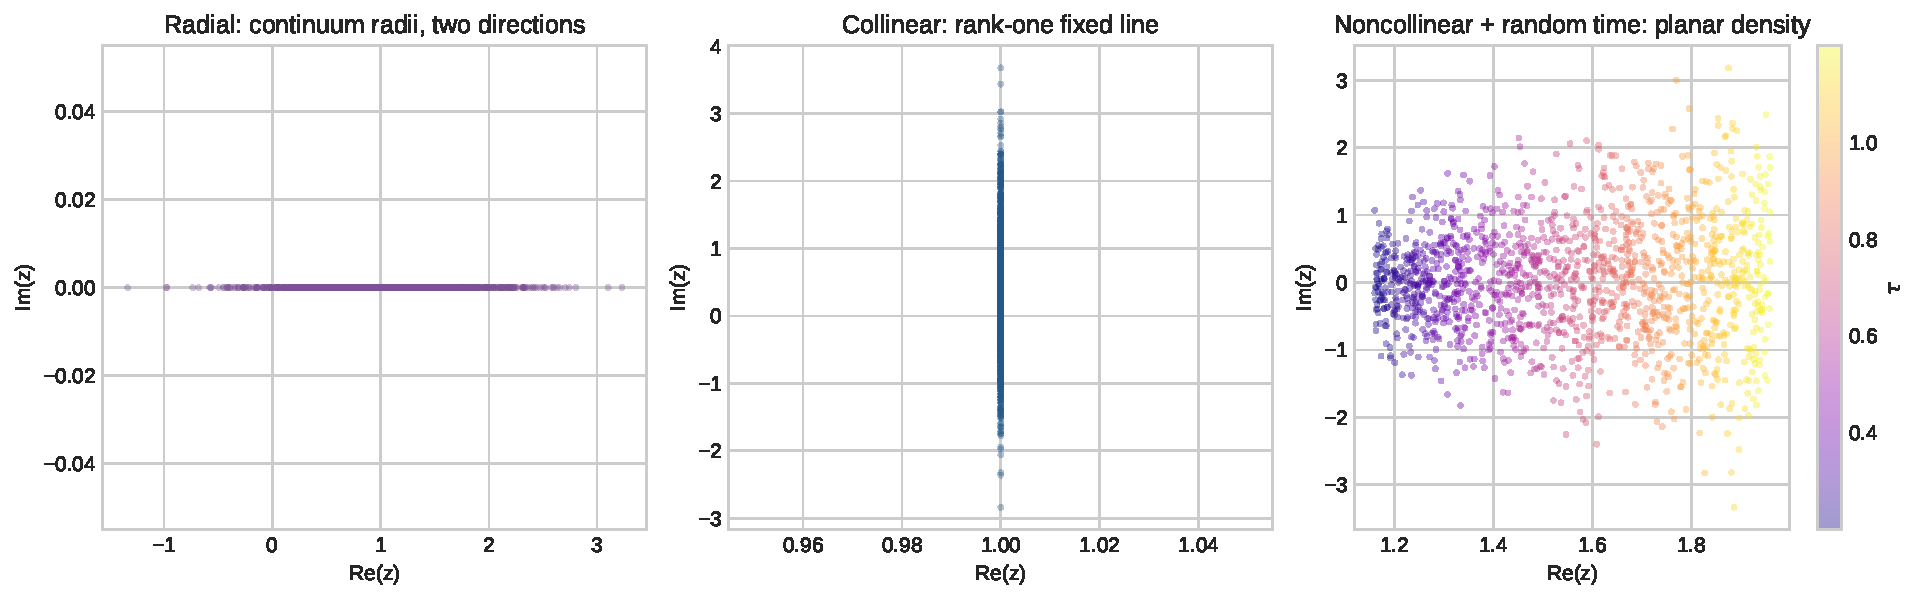
\includegraphics[width=1\linewidth,height=\textheight,keepaspectratio,alt={Three scatter plots: a radial line with two directions, an eligible fixed affine line, and a noncollinear drift-diffusion process whose randomized-time law fills a planar region.}]{figures/vector/f03_support_obstructions.pdf}

}

\caption{\label{fig-support-obstructions}Radial, eligible collinear, and
randomized-time noncollinear support geometries.}

\end{figure}%

The covariance-rank contrast in Figure~\ref{fig-support-obstructions} is
illustrative, not the proof. In the reproducible experiment, the radial
and eligible lines had empirical rank one, while the randomized-time
noncollinear law had positive small eigenvalue \(0.0531\) and
determinant \(0.0370\).

\begin{figure}[tbp]

\centering{

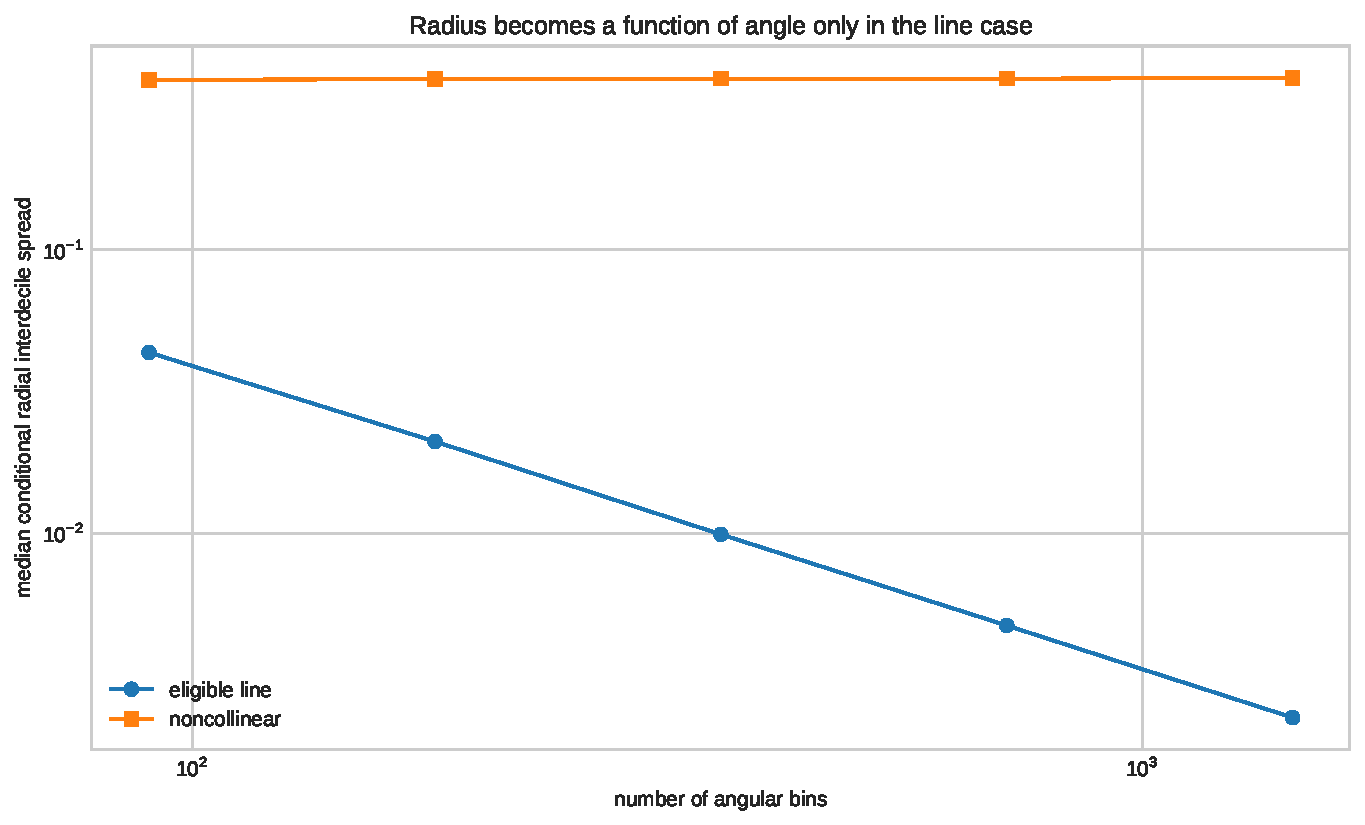
\includegraphics[width=0.78\linewidth,height=\textheight,keepaspectratio,alt={Log-log plot of median conditional radial spread against angular-bin count. The spread tends toward zero for the eligible line but remains large for the noncollinear process.}]{figures/vector/f04_angle_bin_factorization.pdf}

}

\caption{\label{fig-angle-factorization}Conditional radial spread as
angular bins are refined for an eligible line and a noncollinear
randomized-time law.}

\end{figure}%

Figure~\ref{fig-angle-factorization} provides a second diagnostic. As
angular bins are refined, conditional radial dispersion decays for a
line on which radius is a function of angle; it remains substantial for
a planar distribution. The diagnostic visualizes
Eq.~\ref{eq-fiber-condition} and does not replace
Lemma~\ref{lem-polar-graph-null}.

\section{Exact affine classification}\label{sec-classification}

Normalize the process by \(Z_0\):

\begin{equation}\protect\phantomsection\label{eq-normalized-affine}{
\zeta_t:=\frac{Z_t}{Z_0}
=1+\alpha t+cW_t,
\qquad
\alpha=\frac a{Z_0},\quad c=\frac b{Z_0}.
}\end{equation}

\begin{theorem}[Lossless time-independent affine
classification]\protect\hypertarget{thm-affine-classification}{}\label{thm-affine-classification}

Assume \(Z_0b\ne0\) and require Definition
Definition~\ref{def-one-phase} on every deterministic time in a
nontrivial interval. Then

\[
Z_t=Z_0r(\theta_t)e^{i\theta_t}
\]

exists if and only if

\begin{equation}\protect\phantomsection\label{eq-affine-iff}{
\boxed{
\frac ab\in\mathbb R
\quad\text{and}\quad
\frac b{Z_0}\notin\mathbb R.
}
}\end{equation}

Equivalently,

\[
\operatorname{Im}(a\overline b)=0,
\qquad
\operatorname{Im}(b\overline{Z_0})\ne0.
\]

\end{theorem}

\subsection{Sufficiency and explicit
construction}\label{sufficiency-and-explicit-construction}

Assume \(a=\lambda b\) with \(\lambda\in\mathbb R\), and write

\[
c=\frac b{Z_0}=\rho e^{i\phi},
\qquad
\rho>0,\qquad
\sin\phi\ne0.
\]

Then

\begin{equation}\protect\phantomsection\label{eq-affine-scalar-state}{
\zeta_t=1+cx_t,\qquad x_t=\lambda t+W_t.
}\end{equation}

The line \(L=\{1+cx:x\in\mathbb R\}\) misses the origin. Its continuous
argument \(\theta(x)\), anchored by \(\theta(0)=0\), satisfies

\begin{equation}\protect\phantomsection\label{eq-angle-derivative}{
\frac{d\theta}{dx}
=\operatorname{Im}\frac{c}{1+cx}
=\frac{\operatorname{Im}c}{|1+cx|^2},
}\end{equation}

which has fixed nonzero sign. Hence \(\theta\) is strictly monotone and
lossless.

Write \(1+\rho e^{i\phi}x=re^{i\theta}\). Multiplication by
\(e^{-i\phi}\) and comparison of imaginary parts give

\[
r\sin(\theta-\phi)=-\sin\phi.
\]

Therefore

\begin{equation}\protect\phantomsection\label{eq-general-radius-inverse}{
\boxed{
r(\theta)=\frac{\sin\phi}{\sin(\phi-\theta)},
\qquad
x(\theta)
=\frac{\sin\theta}{\rho\sin(\phi-\theta)}.
}
}\end{equation}

Substitution into Eq.~\ref{eq-affine-scalar-state} proves the
representation and its inverse.

\subsection{Necessity of drift-diffusion
collinearity}\label{necessity-of-drift-diffusion-collinearity}

Suppose instead that \(\operatorname{Im}(a\overline b)\ne0\). Choose an
independent random time \(\tau\) uniformly distributed on
\([t_0,t_1]\subset(0,\infty)\). The pair \((\tau,W_\tau)\) has density

\begin{equation}\protect\phantomsection\label{eq-random-time-density}{
f_{\tau,W_\tau}(t,w)
=
\frac{\mathbf 1_{[t_0,t_1]}(t)}{t_1-t_0}
\frac{1}{\sqrt{2\pi t}}
\exp\!\left(-\frac{w^2}{2t}\right).
}\end{equation}

The real-affine map

\[
(t,w)\longmapsto Z_0+at+bw
\]

has nonzero real determinant, equal up to orientation to
\(\operatorname{Im}(a\overline b)\). Thus \(Z_\tau\) is absolutely
continuous with respect to planar Lebesgue measure.

If one time-independent polar graph represented \(Z_t\) almost surely
for every deterministic \(t\in[t_0,t_1]\), Fubini's theorem would give
\(\mathbb P(Z_\tau\in Z_0C_r)=1\). By Lemma~\ref{lem-polar-graph-null}
and planar absolute continuity, the same probability must be zero, a
contradiction. Therefore \(a/b\in\mathbb R\).

Randomizing time is not cosmetic. It closes the quantifier gap in an
informal argument that an uncountable family of support lines ``fills an
area''; an uncountable union of null events cannot otherwise be handled
by countable probability arguments.

\subsection{Necessity that the fixed line miss the
origin}\label{necessity-that-the-fixed-line-miss-the-origin}

Under \(a/b\in\mathbb R\), all supports coincide with
\(L=Z_0+b\mathbb R\). If \(b/Z_0\in\mathbb R\), the normalized line
passes through the origin. Every nonzero point then has geometric
argument \(0\) or \(\pi\) modulo \(2\pi\). Any genuine unwrapped phase
belongs to the countable set

\[
\{2\pi k:k\in\mathbb Z\}
\cup
\{\pi+2\pi k:k\in\mathbb Z\}.
\]

A single-valued \(r\) maps this set to only countably many points. At
every \(t>0\), however, \(Z_t\) has a nonatomic Gaussian law along the
entire line. That law cannot be countably supported. Hence
\(b/Z_0\notin\mathbb R\). Together with the construction above, this
proves Theorem~\ref{thm-affine-classification}. \(\square\)

\subsection{Phase domain and
uniqueness}\label{phase-domain-and-uniqueness}

The exact phase interval is

\begin{equation}\protect\phantomsection\label{eq-general-phase-domain}{
\boxed{
I_\phi=
\begin{cases}
(\phi-\pi,\phi),&\sin\phi>0,\\[3pt]
(\phi,\phi+\pi),&\sin\phi<0.
\end{cases}
}
}\end{equation}

It is the unique open interval of length \(\pi\) containing zero on
which Eq.~\ref{eq-general-radius-inverse} has positive radius. The map
\(x\mapsto\theta\) is a bijection from \(\mathbb R\) to \(I_\phi\), and

\[
|x(\theta)|\to\infty,\qquad r(\theta)\to\infty
\]

at its endpoints. A continuous genuine argument lift is unique after
\(\theta(0)=0\) is fixed. Discontinuous additions of state-dependent
multiples of \(2\pi\) are artificial encodings and do not define the
continuous diffusion coordinate studied here.

\begin{figure}[tbp]

\centering{

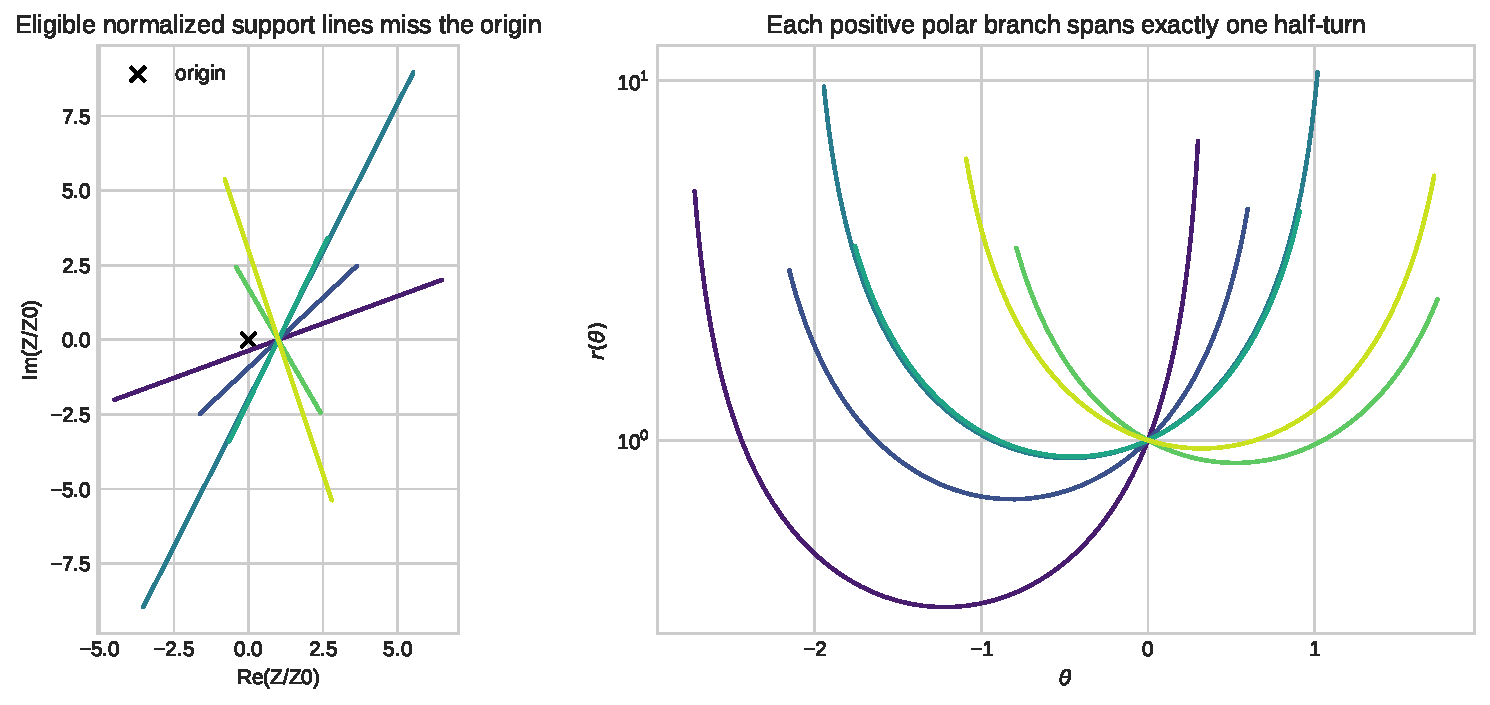
\includegraphics[width=1\linewidth,height=\textheight,keepaspectratio,alt={Left: several normalized affine lines that miss the origin. Right: corresponding positive radius functions over open phase intervals of length pi, shown on a logarithmic scale.}]{figures/vector/f02_general_affine_geometry.pdf}

}

\caption{\label{fig-general-affine}Six eligible oblique affine lines and
their positive phase-radius branches.}

\end{figure}%

The random-parameter reconstruction in Figure~\ref{fig-general-affine}
reached maximum scalar inverse error below \(3.3\times10^{-13}\) and
maximum complex error below \(6.0\times10^{-13}\) across six eligible
lines. These are floating-point checks of an already proved identity.

\subsection{Degenerate and exceptional
cases}\label{degenerate-and-exceptional-cases}

The assumptions in Theorem~\ref{thm-affine-classification} are
substantive.

\begin{itemize}
\tightlist
\item
  If \(b=0\), the process is deterministic. A stochastic phase is
  unnecessary; a time-independent polar graph may or may not contain the
  deterministic trajectory, depending on \(a\) and the interval.
\item
  If \(Z_0=0\), the normalization in Eq.~\ref{eq-requested-form} is
  undefined. One may choose another nonzero reference point, but that is
  a different representation problem.
\item
  If \(a=0\) and \(b/Z_0\notin\mathbb R\), the theorem remains valid
  with \(\lambda=0\).
\item
  If the line passes through the origin, a local polar chart can exist
  on one ray before a crossing, but it is not a global, lossless
  representation of the full Gaussian support.
\item
  If \(a/b\notin\mathbb R\), a time-dependent radius can represent each
  nonsingular fixed-time support line. It uses \((t,\theta)\) rather
  than one time-independent phase and fails when the moving line crosses
  the origin.
\end{itemize}

\begin{figure}[tbp]

\centering{

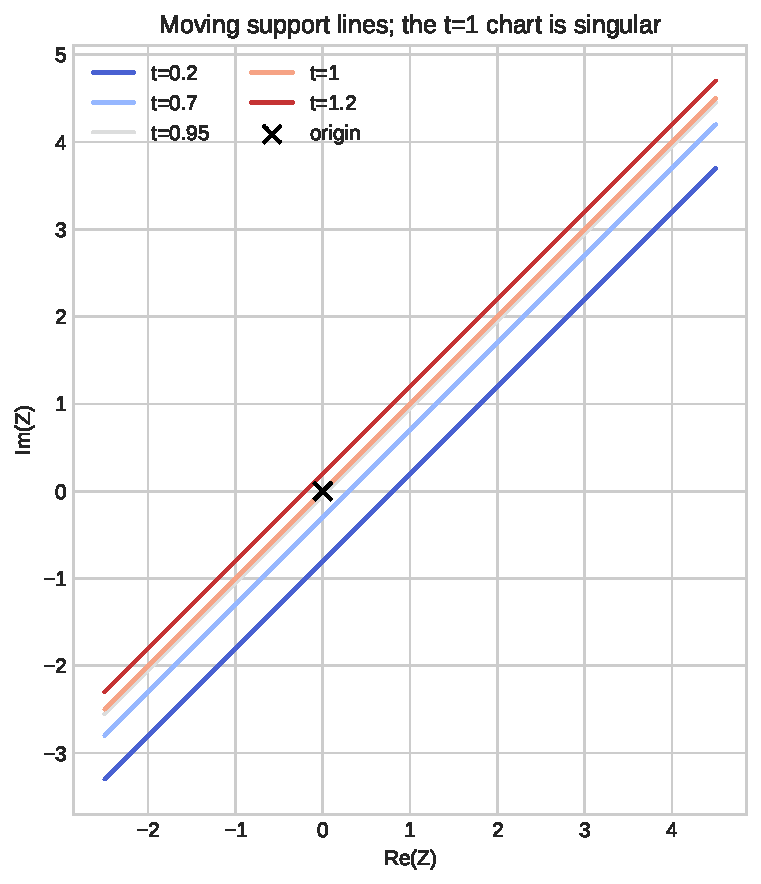
\includegraphics[width=0.88\linewidth,height=\textheight,keepaspectratio,alt={Several time-indexed affine support lines reconstructed with time-dependent polar radii, with a highlighted time at which the line crosses the origin and the chart becomes singular.}]{figures/vector/f13_moving_line_fallback.pdf}

}

\caption{\label{fig-moving-line}Time-dependent polar reconstruction for
moving support lines and the singular origin-crossing time.}

\end{figure}%

Figure~\ref{fig-moving-line} illustrates the last exception. It is a
useful fallback, but it does not satisfy the one-phase problem posed in
Definition Definition~\ref{def-one-phase}.

\section{Canonical secant and constant-radius
charts}\label{sec-canonical}

\subsection{Arithmetic Brownian factor as one Euler
phase}\label{arithmetic-brownian-factor-as-one-euler-phase}

Let

\begin{equation}\protect\phantomsection\label{eq-arithmetic-brownian}{
dX_t=\mu\,dt+\sigma\,dW_t,\qquad X_0\in\mathbb R,
}\end{equation}

and set \(Y_t=X_t-X_0\). For any scale \(c>0\), define the auxiliary
complex state

\begin{equation}\protect\phantomsection\label{eq-canonical-embedding}{
\mathcal Z_t
=Z_0\left(1+i\frac{Y_t}{c}\right).
}\end{equation}

With

\begin{equation}\protect\phantomsection\label{eq-canonical-phase}{
\theta_t=\arctan(Y_t/c)
\in\left(-\frac\pi2,\frac\pi2\right),
}\end{equation}

the exact pathwise representation is

\begin{equation}\protect\phantomsection\label{eq-canonical-reconstruction}{
\boxed{
\mathcal Z_t=Z_0\sec\theta_t\,e^{i\theta_t},
\qquad
X_t=X_0+c\tan\theta_t.
}
}\end{equation}

This is Eq.~\ref{eq-general-radius-inverse} with \(\rho=1/c\) and
\(\phi=\pi/2\). If it is desirable for the real Brownian factor to be
the real rather than imaginary coordinate, one may instead use
\(\widetilde Z_t=ic+Y_t\) and \(\widetilde\theta_t=-\arctan(Y_t/c)\).
These embeddings differ by a rigid rotation and scale.

Equation Eq.~\ref{eq-canonical-reconstruction} answers the
state-representation question in the requested form: neither \(t\) nor
\(W_t\) appears separately on its right-hand side. They remain present
in the law of \(\theta\), as they must. The sigma-fields generated by
the current states agree,

\[
\sigma(\theta_t)=\sigma(X_t),
\]

and the completed path filtrations agree because both transforms are
continuous and invertible.

\subsection{Geometry of the secant
curve}\label{geometry-of-the-secant-curve}

Let \(F(\theta)=\sec\theta e^{i\theta}=1+i\tan\theta\). Then

\[
F'(\theta)=i\sec^2\theta,\qquad
F''(\theta)=2i\sec^2\theta\tan\theta.
\]

The signed curvature,

\[
\kappa(\theta)
=
\frac{\operatorname{Im}\{\overline{F'(\theta)}F''(\theta)\}}
{|F'(\theta)|^3},
\]

is identically zero. Thus the algebraic factors ``radius'' and
``rotation'' conspire to trace a line. The stochastic phase is
genuine---it is the angle of the point relative to the origin---but it
is confined to one open half-turn.

The scale \(c\) does not change the information carried by the chart. It
controls where physical values are allocated in phase:

\[
\frac{d\theta}{dx}=\frac{c}{c^2+x^2}.
\]

Small \(c\) allocates more angular resolution near zero and compresses
tails more aggressively; large \(c\) is closer to linear on a wider
physical region. This tuning later affects PDE resolution and
conditioning.

\subsection{Cayley constant-radius
alternative}\label{cayley-constant-radius-alternative}

A constant radius is possible after changing the represented state.
Define

\begin{equation}\protect\phantomsection\label{eq-cayley-transform}{
U_t
=
\frac{1+iY_t/c}{1-iY_t/c}
=e^{i\Theta_t},
\qquad
\Theta_t=2\arctan(Y_t/c)\in(-\pi,\pi).
}\end{equation}

Because the denominator is the complex conjugate of the numerator,
\(|U_t|=1\), and

\[
Y_t=c\tan(\Theta_t/2).
\]

The point \(U=-1\) represents infinity and is inaccessible at every
finite time. This construction keeps constant radius and losslessness on
\(S^1\setminus\{-1\}\), but it represents a nonlinear transform of
Eq.~\ref{eq-canonical-embedding}, not the original additive complex
state.

\begin{figure}[tbp]

\centering{

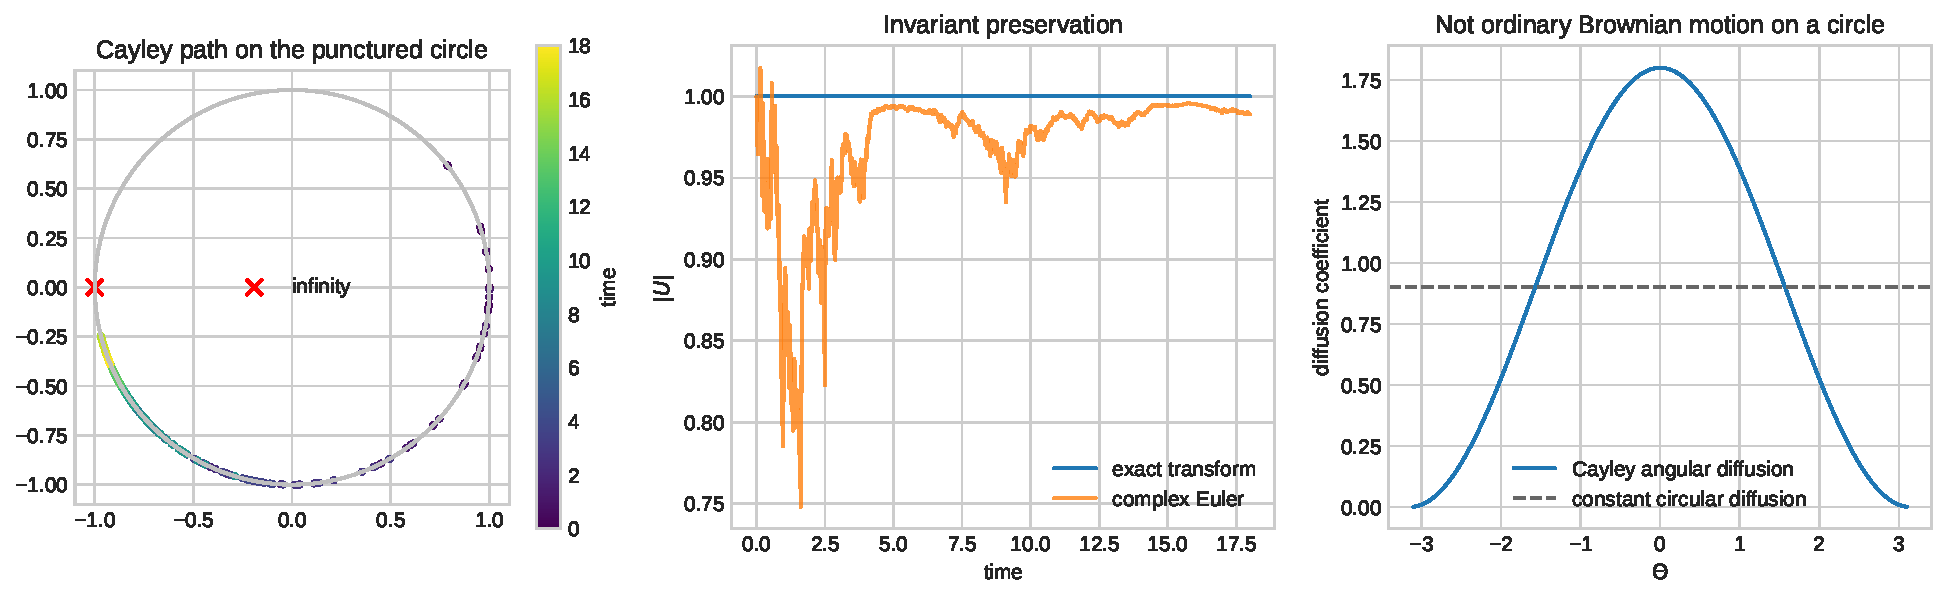
\includegraphics[width=1\linewidth,height=\textheight,keepaspectratio,alt={Panels showing the Cayley map of the real line onto a punctured unit circle, exact modulus preservation compared with an unconstrained numerical control, and angular diffusion decaying near the missing point.}]{figures/vector/f09_cayley_compactification.pdf}

}

\caption{\label{fig-cayley}Cayley compactification, exact unit-modulus
preservation, and the state-dependent angular diffusion near the missing
point.}

\end{figure}%

The executed experiment in Figure~\ref{fig-cayley} found maximum exact
modulus defect \(4.44\times10^{-16}\) and inverse error
\(1.78\times10^{-15}\), whereas an unconstrained complex Euler control
accumulated modulus error \(0.252\). That is a structure-preservation
benefit for the transformed state. It does not make \(\Theta\) standard
Brownian motion on the circle: its angular diffusion is state dependent
and vanishes near the missing point.

\section{Phase diffusion, generator, kernel, and
boundaries}\label{sec-phase-theory}

\subsection{Canonical Itô and Stratonovich
equations}\label{canonical-ituxf4-and-stratonovich-equations}

For \(f(x)=\arctan(x/c)\),

\[
f'(x)=\frac{c}{c^2+x^2},
\qquad
f''(x)=-\frac{2cx}{(c^2+x^2)^2}.
\]

Applying Itô's formula to Eq.~\ref{eq-arithmetic-brownian} and
substituting \(X-X_0=c\tan\theta\) gives

\begin{equation}\protect\phantomsection\label{eq-canonical-phase-sde}{
\boxed{
d\theta_t
=
\left[
\frac{\mu}{c}\cos^2\theta_t
-
\frac{\sigma^2}{c^2}
\sin\theta_t\cos^3\theta_t
\right]dt
+
\frac{\sigma}{c}\cos^2\theta_t\,dW_t.
}
}\end{equation}

\begin{equation}\protect\phantomsection\label{eq-phase-coefficients}{
A(\theta)
=
\frac{\mu}{c}\cos^2\theta
-
\frac{\sigma^2}{c^2}\sin\theta\cos^3\theta,
\qquad
B(\theta)=\frac{\sigma}{c}\cos^2\theta.
}\end{equation}

Its Stratonovich form is simpler:

\begin{equation}\protect\phantomsection\label{eq-phase-stratonovich}{
\boxed{
d\theta_t
=
\frac{\mu}{c}\cos^2\theta_t\,dt
+
\frac{\sigma}{c}\cos^2\theta_t\circ dW_t.
}
}\end{equation}

The Itô correction is not optional. Since
\(\frac12BB'=-(\sigma^2/c^2)\sin\theta\cos^3\theta\), converting
Eq.~\ref{eq-phase-stratonovich} to Itô produces exactly the second term
in Eq.~\ref{eq-phase-coefficients}.

Conversely, apply Itô's formula to \(F(\theta)=1+i\tan\theta\) under
Eq.~\ref{eq-canonical-phase-sde}. The nonlinear drift from
\(F'\,d\theta\) cancels the \(\frac12F''\,d[\theta,\theta]\) term,
leaving

\begin{equation}\protect\phantomsection\label{eq-two-way-ito}{
d\{Z_0F(\theta_t)\}
=\frac{iZ_0}{c}\left(\mu\,dt+\sigma\,dW_t\right),
}\end{equation}

which reconstructs Eq.~\ref{eq-canonical-embedding}. This two-way
calculation is the precise connection between Brownian quadratic
variation and the complex curve: quadratic variation produces a
geometric drift correction through \(F''\). It is not identified with
\(i^2\).

\subsection{General affine phase
equation}\label{general-affine-phase-equation}

For the eligible general line, define

\begin{equation}\protect\phantomsection\label{eq-general-g}{
g(\theta)
:=
\frac{\rho\sin^2(\phi-\theta)}{\sin\phi}.
}\end{equation}

By Eq.~\ref{eq-angle-derivative} and
Eq.~\ref{eq-general-radius-inverse}, \(d\theta/dx=g(\theta)\) and

\[
g'(\theta)
=
-\frac{2\rho\sin(\phi-\theta)\cos(\phi-\theta)}
{\sin\phi}.
\]

Since \(dx_t=\lambda\,dt+dW_t\),

\begin{equation}\protect\phantomsection\label{eq-general-phase-sde}{
\boxed{
d\theta_t
=
\left[
\lambda g(\theta_t)
+\frac12g(\theta_t)g'(\theta_t)
\right]dt
+g(\theta_t)dW_t,
}
}\end{equation}

or, in Stratonovich form,

\[
d\theta_t
=\lambda g(\theta_t)dt+g(\theta_t)\circ dW_t.
\]

The sign of \(g\) records orientation. A scalar diffusion coefficient
need not be declared positive; reversing \(W\) reverses its sign without
changing the law.

\subsection{Generator and phase-first
specification}\label{generator-and-phase-first-specification}

The canonical generator is

\begin{equation}\protect\phantomsection\label{eq-phase-generator}{
\boxed{
\mathcal L_\theta h
=A(\theta)h'(\theta)
+\frac12B(\theta)^2h''(\theta),
}
}\end{equation}

with \(A,B\) from Eq.~\ref{eq-phase-coefficients}. The martingale
problem for Eq.~\ref{eq-phase-generator} on \((-\pi/2,\pi/2)\) defines
the phase law without naming \(t\) or \(W_t\) as state coordinates.
Equivalently, its Markov transition kernel specifies the law. This is
the rigorous interpretation of ``\(\theta_t\) is the only stochastic
state variable'': the process remains time-indexed and random, but its
Markov state is one scalar.

\subsection{Exact transition density and
semigroup}\label{exact-transition-density-and-semigroup}

\begin{theorem}[Canonical transition
kernel]\protect\hypertarget{thm-phase-kernel}{}\label{thm-phase-kernel}

For \(\sigma\ne0\), \(u,v\in(-\pi/2,\pi/2)\), and \(h>0\), the
transition density of Eq.~\ref{eq-canonical-phase-sde} is

\begin{equation}\protect\phantomsection\label{eq-phase-kernel}{
\boxed{
p_h(v\mid u)
=
\frac{c\sec^2v}{|\sigma|\sqrt{2\pi h}}
\exp\!\left[
-\frac{
\left(c\tan v-c\tan u-\mu h\right)^2
}{2\sigma^2h}
\right].
}
}\end{equation}

\end{theorem}

\textbf{Proof.} Conditional on \(\theta_s=u\),

\[
X_{s+h}-X_0
=c\tan u+\mu h+\sigma\sqrt h\,\xi,
\qquad \xi\sim N(0,1).
\]

The inverse \(v=\arctan((X-X_0)/c)\) has Jacobian \(dX/dv=c\sec^2v\),
giving Eq.~\ref{eq-phase-kernel}. \(\square\)

The exact step is therefore

\begin{equation}\protect\phantomsection\label{eq-exact-phase-step}{
\boxed{
\theta_{s+h}
=
\arctan\!\left(
\tan\theta_s+\frac{\mu h}{c}
+\frac{\sigma\sqrt h}{c}\xi
\right).
}
}\end{equation}

For the general line, using the inverse \(x(\theta)\) in
Eq.~\ref{eq-general-radius-inverse},

\begin{equation}\protect\phantomsection\label{eq-general-phase-kernel}{
p_h(v\mid u)
=
\frac{|x'(v)|}{\sqrt{2\pi h}}
\exp\!\left[
-\frac{(x(v)-x(u)-\lambda h)^2}{2h}
\right],
}\end{equation}

where

\[
|x'(v)|
=\frac{|\sin\phi|}{\rho\sin^2(\phi-v)}.
\]

Normalization follows by substituting \(y=x(v)\). The
Chapman--Kolmogorov identity follows from Gaussian convolution under the
same substitution. Thus the ``new'' phase kernel is exactly the known
Gaussian kernel pushed through a diffeomorphism; it is not a newly
solved diffusion.

\begin{figure}[tbp]

\centering{

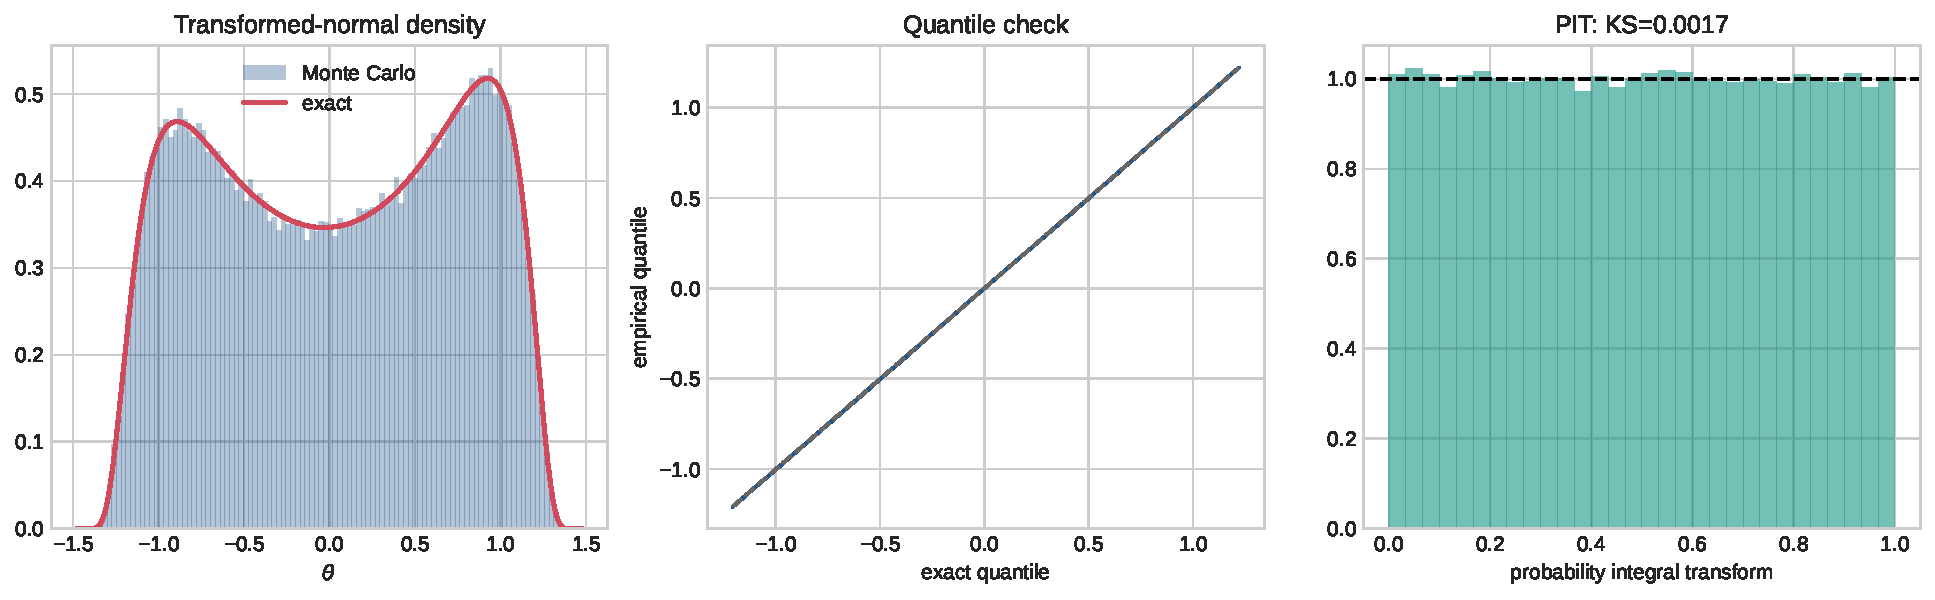
\includegraphics[width=1\linewidth,height=\textheight,keepaspectratio,alt={Panels comparing the analytic phase transition density with simulated data, a probability-integral-transform diagnostic, and direct versus composed semigroup values.}]{figures/vector/f07_transition_diagnostics.pdf}

}

\caption{\label{fig-transition-diagnostics}Transition-density
normalization, probability-integral-transform diagnostics, and semigroup
consistency.}

\end{figure}%

In Figure~\ref{fig-transition-diagnostics}, numerical quadrature
returned mass \(0.9999999999999999\), direct and composed semigroup
values differed by \(1.11\times10^{-16}\), and the
probability-integral-transform KS statistic was \(0.00173\) with
\(p=0.726\). A separate finite-difference forward-equation check had
relative RMS residual \(6.90\times10^{-5}\).

\subsection{Natural phase boundaries}\label{natural-phase-boundaries}

The endpoints \(\pm\pi/2\) correspond under \(x=c\tan\theta\) to
\(\pm\infty\). For every finite \(T\),

\[
\sup_{0\le t\le T}|X_t|
\le
|X_0|+|\mu|T+|\sigma|
\sup_{0\le t\le T}|W_t|
<\infty
\quad\text{a.s.}
\]

Therefore neither phase endpoint is reached from the interior in finite
time. Nor is either an entrance: for any compact \(K\subset\mathbb R\)
and \(t>0\),

\[
\mathbb P_x(X_t\in K)\longrightarrow0
\qquad\text{as }x\to\pm\infty.
\]

The Gaussian transition laws escape every compact set and have no
probability limit on \(\mathbb R\) from which a Feller entrance law can
be defined. In the standard one-dimensional classification, both
endpoints are natural (Feller 1954). Smooth monotone conjugacy preserves
the classification, so

\begin{equation}\protect\phantomsection\label{eq-natural-boundaries}{
\boxed{
-\frac\pi2\text{ and }\frac\pi2
\text{ are inaccessible natural boundaries.}
}
}\end{equation}

The same statement holds for the endpoints of \(I_\phi\). No reflecting
or absorbing boundary condition should be imposed on the exact
diffusion.

\begin{figure}[tbp]

\centering{

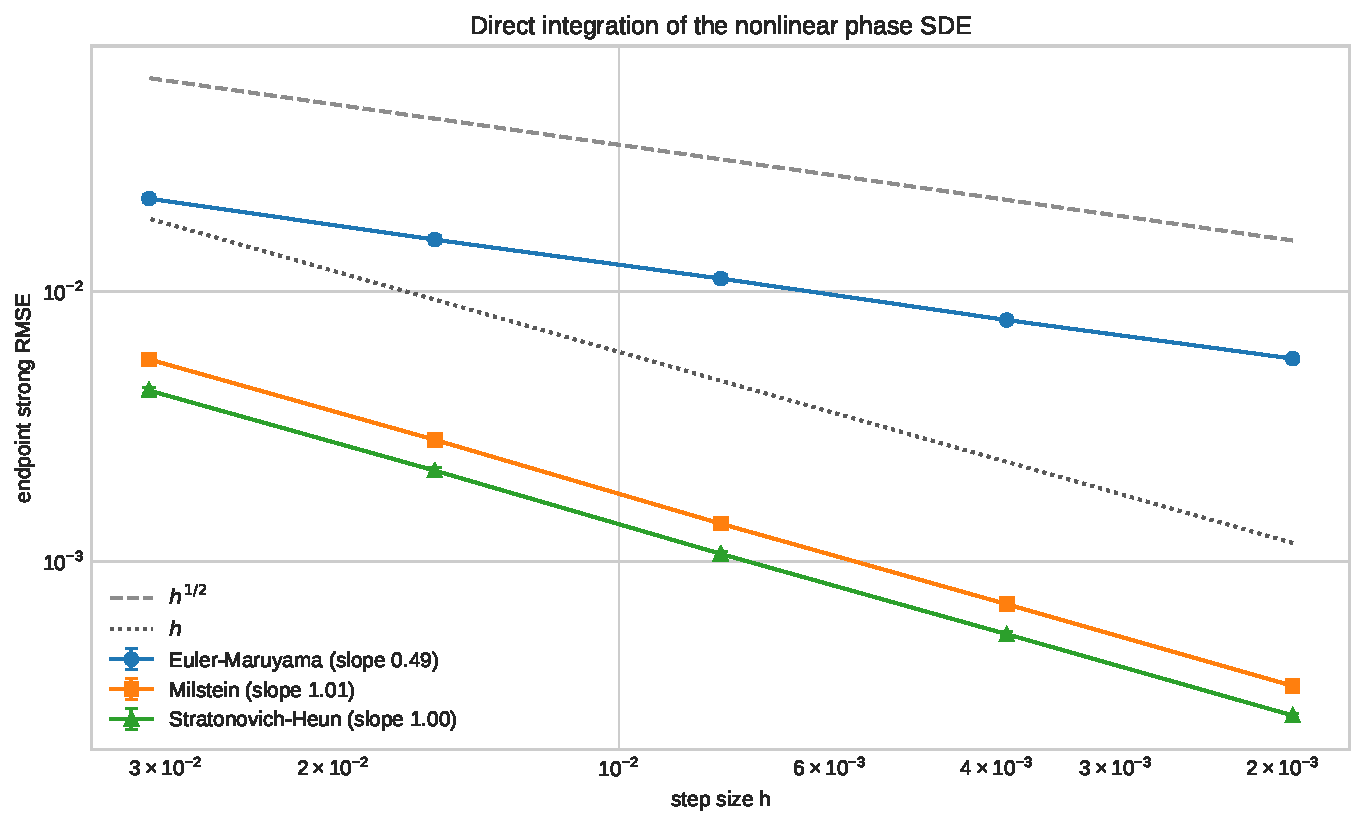
\includegraphics[width=0.85\linewidth,height=\textheight,keepaspectratio,alt={Log-log strong-error plots for Euler--Maruyama, Milstein, and Stratonovich--Heun against their exact transformed-Gaussian reference, together with fitted slopes.}]{figures/vector/f05_phase_sde_convergence.pdf}

}

\caption{\label{fig-phase-convergence}Strong convergence of independent
nonlinear phase schemes and exact phase behavior near the natural
boundaries.}

\end{figure}%

\begin{figure}[tbp]

\centering{

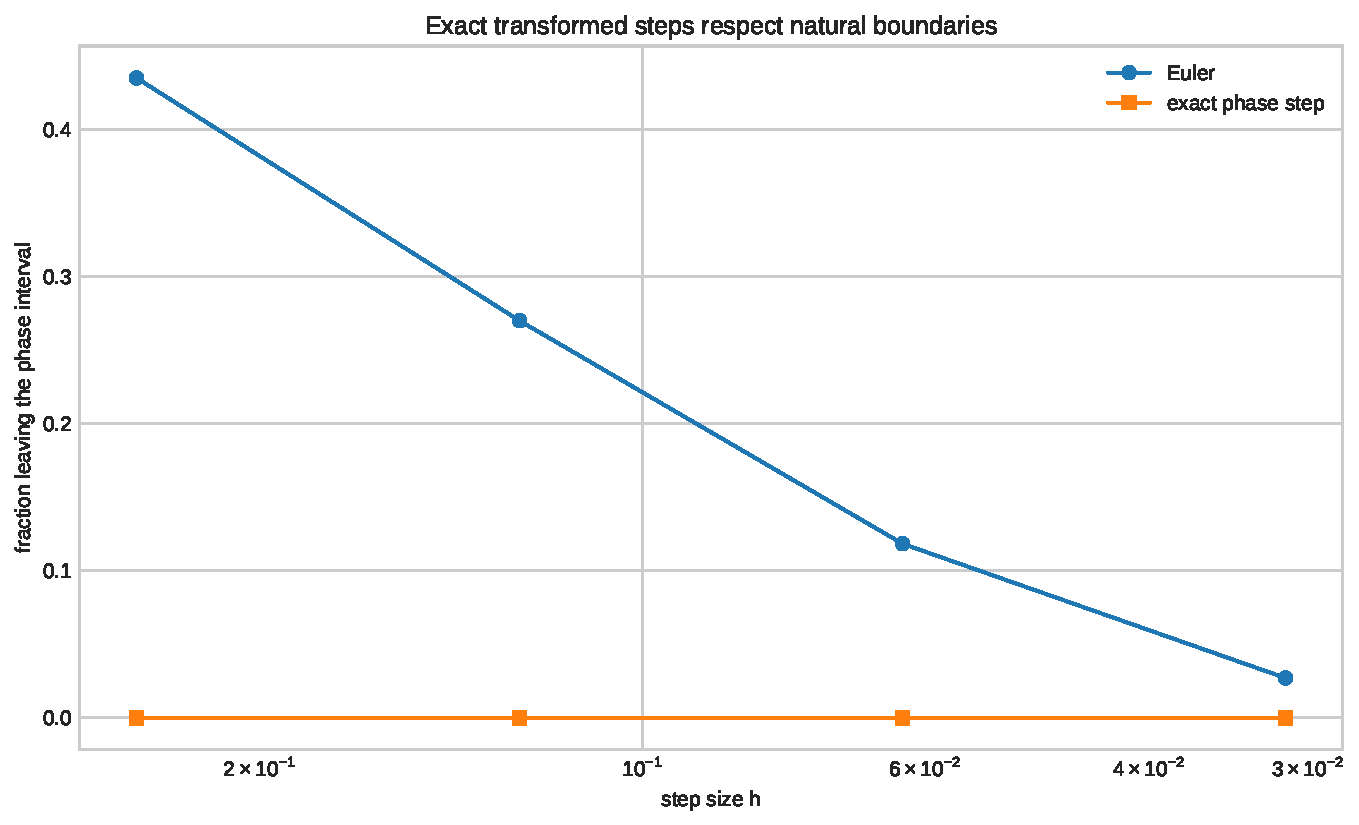
\includegraphics[width=0.85\linewidth,height=\textheight,keepaspectratio,alt={Boundary-violation rates over four step sizes. Exact transformed steps remain inside the open phase interval, while unconstrained Euler steps leave it frequently at coarse resolution.}]{figures/vector/f06_boundary_stress.pdf}

}

\caption{\label{fig-boundary-stress}Boundary stress comparison between
exact transformed steps and unconstrained Euler steps.}

\end{figure}%

The numerical implications of Eq.~\ref{eq-natural-boundaries} are
visible in Figure~\ref{fig-boundary-stress}. Exact transformed steps
remain in the interval by construction. With \(c=0.25\), \(\sigma=1\),
and \(120{,}000\) samples, unconstrained one-step Euler violation rates
fell from \(0.435\) at \(h=0.25\) to \(0.0271\) at \(h=0.03125\).
Bounded coordinates do not make a naive discretization automatically
boundary preserving.

\begin{figure}[tbp]

\centering{

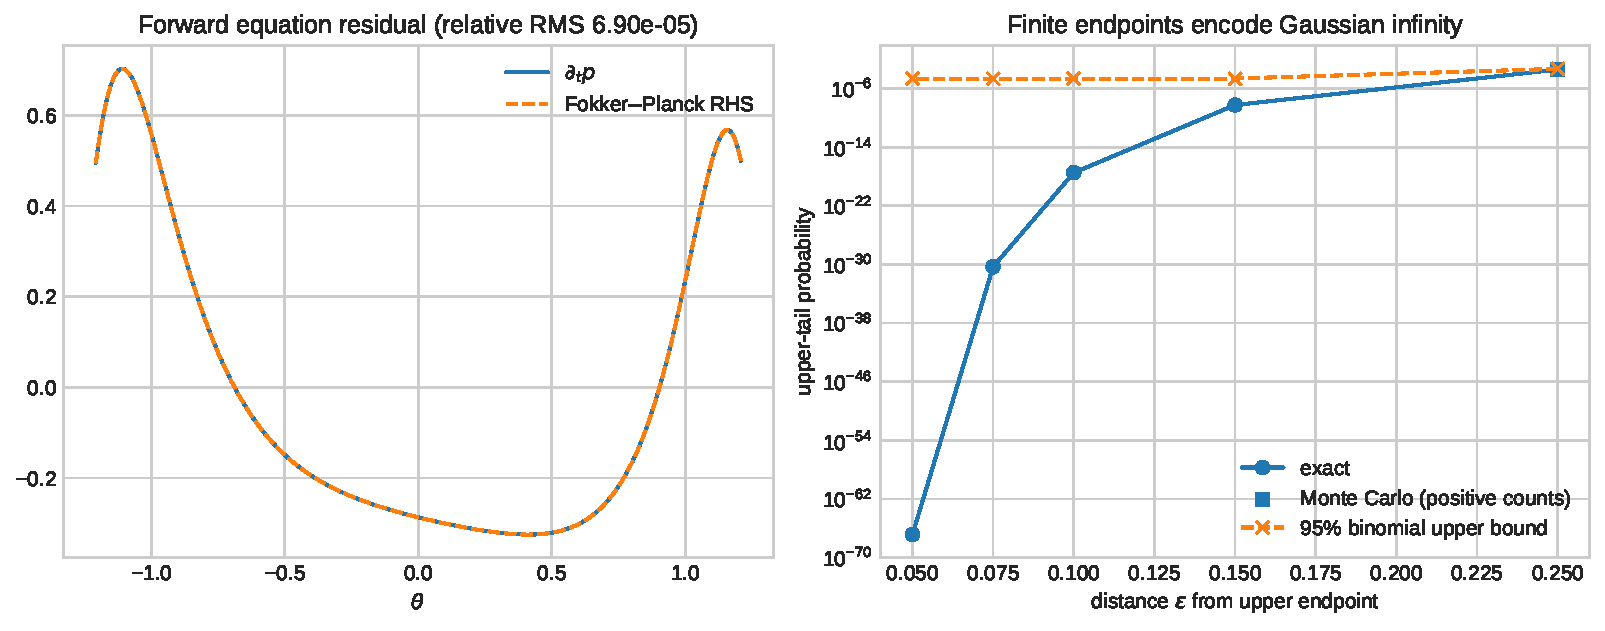
\includegraphics[width=1\linewidth,height=\textheight,keepaspectratio,alt={Panels showing empirical small-time drift and variance approaching theoretical generator coefficients, a Fokker--Planck residual diagnostic, and exact endpoint-tail probabilities with Monte Carlo detection limits.}]{figures/vector/f08_generator_and_endpoint_checks.pdf}

}

\caption{\label{fig-generator-endpoints}Small-time generator estimates,
forward-equation residual, and endpoint-tail diagnostics.}

\end{figure}%

Zero observed rare endpoint events are not interpreted as zero
probability. The notebook reports exact Gaussian tail probabilities and
binomial upper confidence bounds together, as shown in
Figure~\ref{fig-generator-endpoints}.

\section{Additive and multiplicative rigidity}\label{sec-rigidity}

\subsection{Dynamics induced by a phase
curve}\label{dynamics-induced-by-a-phase-curve}

Let

\[
F(\theta)=r(\theta)e^{i\theta},
\qquad r\in C^2(I;(0,\infty)),
\]

and let

\[
d\theta_t=m(\theta_t)\,dt+s(\theta_t)\,dW_t.
\]

For \(Z_t=Z_0F(\theta_t)\), Itô's formula gives

\begin{equation}\protect\phantomsection\label{eq-general-curve-ito}{
\boxed{
dZ_t
=
Z_0\left(F'm+\frac12F''s^2\right)(\theta_t)dt
+Z_0F'(\theta_t)s(\theta_t)dW_t.
}
}\end{equation}

The diffusion coefficient already imposes a strong curve constraint;
matching the drift supplies a second, independent compatibility
equation.

\begin{theorem}[Local additive
rigidity]\protect\hypertarget{thm-additive-rigidity}{}\label{thm-additive-rigidity}

Assume \(F'\ne0\) and \(s\ne0\). The curve-valued process in
Eq.~\ref{eq-general-curve-ito} satisfies

\[
dZ_t=a\,dt+b\,dW_t,\qquad b\ne0,
\]

if and only if

\begin{equation}\protect\phantomsection\label{eq-additive-rigidity}{
F'(\theta)s(\theta)=\frac b{Z_0},
\qquad
\frac ab\in\mathbb R,
\qquad
m(\theta)=\frac ab\,s(\theta)+\frac12s(\theta)s'(\theta).
}\end{equation}

The image of \(F\) lies on a straight line. Every nonradial genuine
polar member has local radius

\[
r(\theta)=\frac{C}{\sin(\delta-\theta)}
\]

on an interval where the expression is positive.

\end{theorem}

\textbf{Proof.} Diffusion matching yields \(F's=b/Z_0\). Differentiation
gives \(F''=-(b/Z_0)s'/s^2\). Drift matching then reduces to

\[
\frac ab=\frac ms-\frac12s'\in\mathbb R,
\]

which is Eq.~\ref{eq-additive-rigidity}. Because \(s\) is real, \(F'\)
always has the fixed complex direction \(b/Z_0\), so \(F(I)\) is a line.
Writing \(F'=e^{i\theta}(r'+ir)\) and fixing the tangent argument
\(\delta\) gives \(r'/r=\cot(\delta-\theta)\); integration yields the
stated radius. \(\square\)

The global origin and losslessness restrictions in
Theorem~\ref{thm-affine-classification} remain necessary. Local tangent
matching alone does not resolve them.

\begin{theorem}[Local multiplicative
rigidity]\protect\hypertarget{thm-multiplicative-rigidity}{}\label{thm-multiplicative-rigidity}

Suppose instead that

\[
dZ_t=A Z_t\,dt+B Z_t\,dW_t,\qquad B=\sigma+i\beta\ne0.
\]

A genuine phase with \(s\ne0\) exists if and only if

\begin{equation}\protect\phantomsection\label{eq-multiplicative-shape}{
\boxed{
\beta\ne0,\qquad
s(\theta)\equiv\beta,\qquad
r(\theta)=r_0e^{k\theta},\qquad
k=\frac{\sigma}{\beta},
}
}\end{equation}

and \(m(\theta)\equiv m_0\in\mathbb R\) satisfies

\begin{equation}\protect\phantomsection\label{eq-multiplicative-drift}{
\boxed{
A=(k+i)m_0+\frac12(k+i)^2\beta^2.
}
}\end{equation}

Equivalently,

\begin{equation}\protect\phantomsection\label{eq-log-collinearity}{
A-\frac12B^2\in B\mathbb R.
}\end{equation}

\end{theorem}

\textbf{Proof.} Diffusion matching gives \((F'/F)s=B\). Since

\[
\frac{F'}F=\frac{r'}r+i,
\]

imaginary parts force \(s=\beta\ne0\), and real parts give
\(r'/r=\sigma/\beta=k\). Thus \(r=r_0e^{k\theta}\). Substituting
\(F'/F=k+i\) and \(F''/F=(k+i)^2\) into the drift equation forces
constant \(m_0\) and Eq.~\ref{eq-multiplicative-drift}. The equivalent
logarithmic condition follows from \(B=(k+i)\beta\). \(\square\)

The line and spiral dictionary is therefore:

\begin{longtable}[]{@{}
  >{\raggedright\arraybackslash}p{(\linewidth - 4\tabcolsep) * \real{0.3333}}
  >{\raggedright\arraybackslash}p{(\linewidth - 4\tabcolsep) * \real{0.3333}}
  >{\raggedright\arraybackslash}p{(\linewidth - 4\tabcolsep) * \real{0.3333}}@{}}
\caption{Additive and multiplicative
rigidity.}\label{tbl-rigidity}\tabularnewline
\toprule\noalign{}
\begin{minipage}[b]{\linewidth}\raggedright
Constant-coefficient law
\end{minipage} & \begin{minipage}[b]{\linewidth}\raggedright
Forced curve
\end{minipage} & \begin{minipage}[b]{\linewidth}\raggedright
Drift compatibility
\end{minipage} \\
\midrule\noalign{}
\endfirsthead
\toprule\noalign{}
\begin{minipage}[b]{\linewidth}\raggedright
Constant-coefficient law
\end{minipage} & \begin{minipage}[b]{\linewidth}\raggedright
Forced curve
\end{minipage} & \begin{minipage}[b]{\linewidth}\raggedright
Drift compatibility
\end{minipage} \\
\midrule\noalign{}
\endhead
\bottomrule\noalign{}
\endlastfoot
\(dZ=a\,dt+b\,dW\) & Straight affine line; secant-type polar radius &
\(a/b\in\mathbb R\) and Eq.~\ref{eq-additive-rigidity} \\
\(dZ/Z=A\,dt+B\,dW\) & Logarithmic spiral
\(r=r_0e^{(\operatorname{Re}B/\operatorname{Im}B)\theta}\) &
\(A-\tfrac12B^2\in B\mathbb R\) \\
\end{longtable}

\begin{figure}[tbp]

\centering{

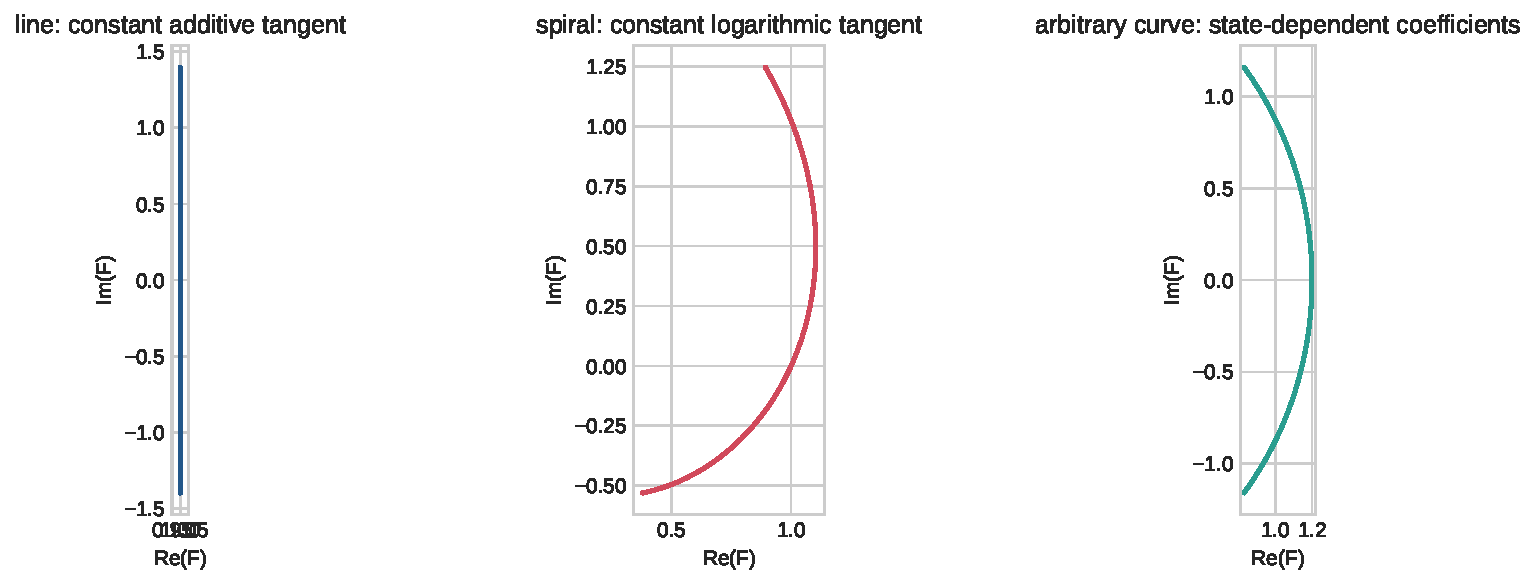
\includegraphics[width=0.88\linewidth,height=\textheight,keepaspectratio,alt={Coefficient residuals for three curve families. The line has zero additive residual, the logarithmic spiral has zero multiplicative residual, and a generic quadratic-radius curve satisfies neither.}]{figures/vector/f12_rigidity_families.pdf}

}

\caption{\label{fig-rigidity-families}Residual checks distinguishing
additive lines, multiplicative logarithmic spirals, and a generic polar
curve.}

\end{figure}%

The numerical residuals in Figure~\ref{fig-rigidity-families} are
controls: \(4.90\times10^{-17}\) for the line/additive match and
\(1.09\times10^{-16}\) for the spiral/multiplicative match. They
illustrate, but do not prove, the coefficient-matching theorems.

\subsection{Winding requires a multiplicative
model}\label{winding-requires-a-multiplicative-model}

For

\begin{equation}\protect\phantomsection\label{eq-complex-log-affine}{
Z_t=Z_0\exp(\kappa t+BW_t),
\qquad B=\sigma+i\beta,
}\end{equation}

condition Eq.~\ref{eq-log-collinearity} says \(\kappa=\gamma B\) for
some \(\gamma\in\mathbb R\). When \(\beta\ne0\),

\begin{equation}\protect\phantomsection\label{eq-spiral-phase}{
\theta_t=\beta(\gamma t+W_t),
\qquad
\boxed{
Z_t
=Z_0\exp\!\left(\frac{\sigma}{\beta}\theta_t\right)e^{i\theta_t}.
}
}\end{equation}

Unlike the additive secant phase, \(\theta\) ranges over the real line
and can wind indefinitely. The price is a change in the stochastic model
from additive affine dynamics to a compatible multiplicative
exponential.

\begin{figure}[tbp]

\centering{

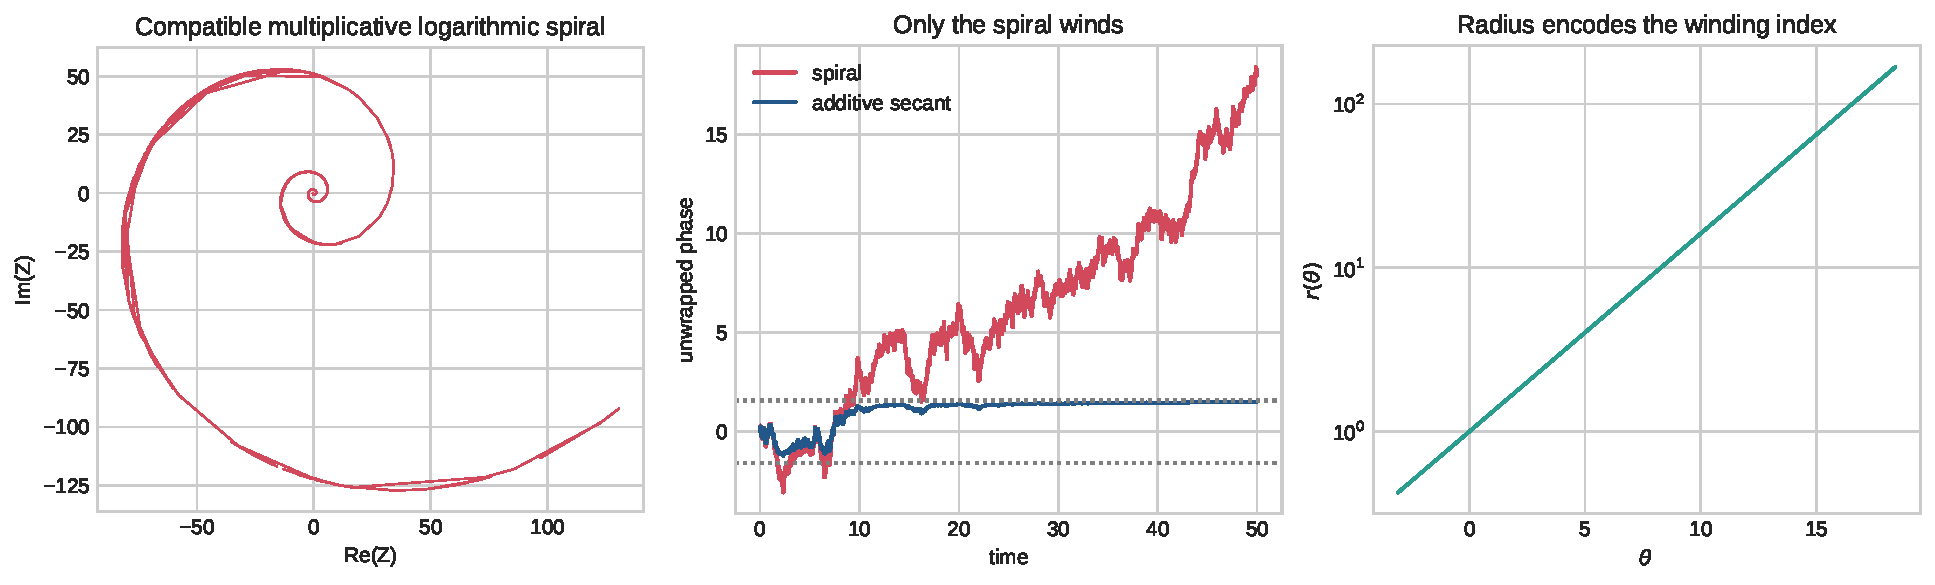
\includegraphics[width=1\linewidth,height=\textheight,keepaspectratio,alt={Side-by-side paths: an additive secant phase remains within one open half-turn, while a compatible multiplicative process winds along a logarithmic spiral with phase on the full real line.}]{figures/vector/f11_additive_vs_spiral.pdf}

}

\caption{\label{fig-additive-spiral}Additive half-turn geometry versus
compatible multiplicative logarithmic-spiral winding.}

\end{figure}%

The simulated spiral in Figure~\ref{fig-additive-spiral} spanned
\(21.49\) radians (\(3.42\) turns), while the additive phase span
remained \(2.72<\pi\). This is a model distinction, not evidence that
one representation is a rewriting of the other.

\subsection{Transported state group}\label{transported-state-group}

The canonical chart

\[
\Phi_c(x)=\arctan(x/c)
\]

transports real addition to

\begin{equation}\protect\phantomsection\label{eq-transported-addition}{
\boxed{
\theta_1\oplus\theta_2
=
\arctan(\tan\theta_1+\tan\theta_2).
}
}\end{equation}

Thus

\[
\left((-\pi/2,\pi/2),\oplus\right)
\cong(\mathbb R,+).
\]

The operation is associative and commutative, has identity zero and
inverse \(-\theta\), and exactly combines scalar increments inside the
bounded chart. It is not ordinary angular addition. Indeed,

\[
(1+ix/c)(1+iy/c)
=1+i(x+y)/c-xy/c^2,
\]

so the secant embedding does not turn addition into ordinary complex
multiplication.

\begin{figure}[tbp]

\centering{

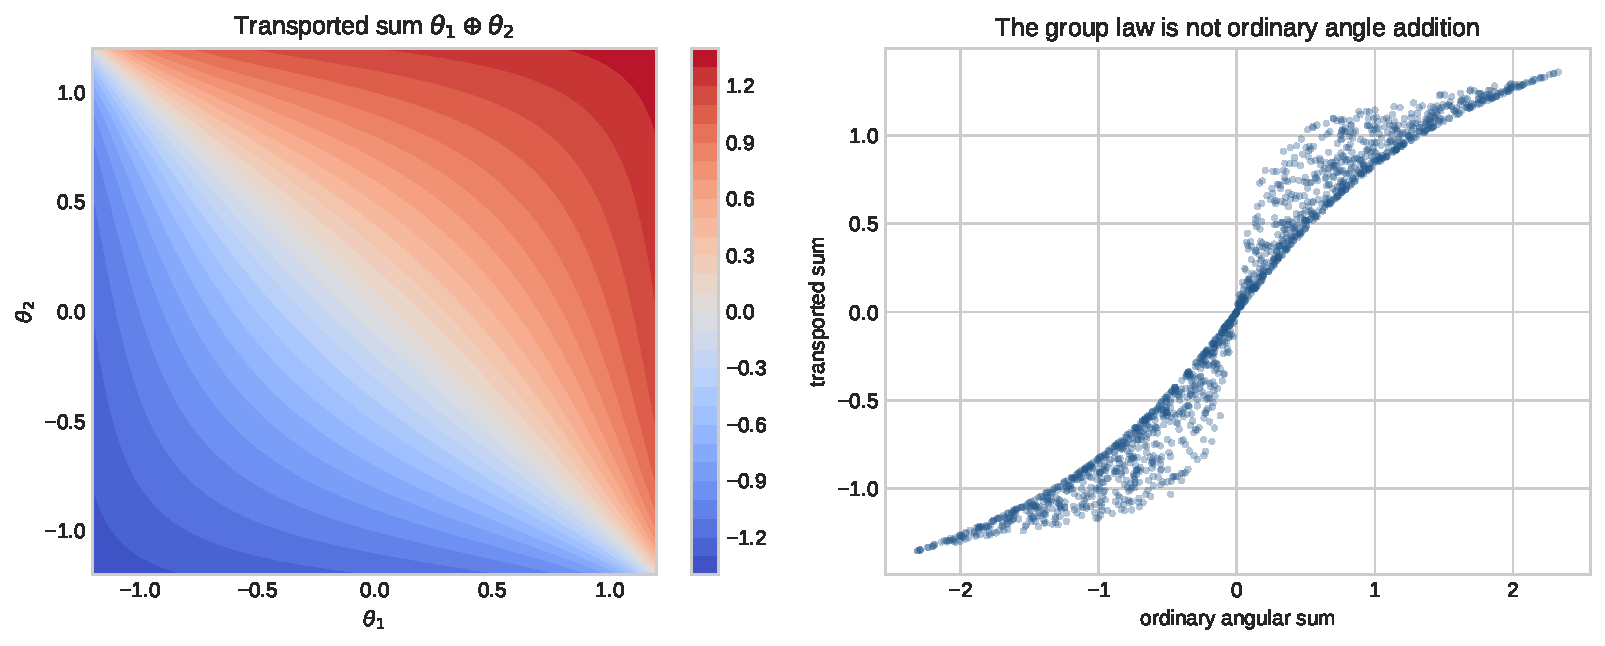
\includegraphics[width=1\linewidth,height=\textheight,keepaspectratio,alt={Plots of the nonlinear transported addition laws in secant and Cayley coordinates, with diagnostics showing exact associativity and a nonzero discrepancy from ordinary angle addition.}]{figures/vector/f10_transported_group.pdf}

}

\caption{\label{fig-transported-group}The transported secant and Cayley
group laws compared with ordinary angular addition.}

\end{figure}%

The notebook verified the tangent-addition identity to
\(3.11\times10^{-15}\) and associativity to \(1.67\times10^{-15}\),
while the RMS discrepancy from ordinary angular addition was \(0.288\).
The group structure comes from conjugated real addition.

There is no continuous injective homomorphism from \((\mathbb R,+)\)
into \((S^1,\cdot)\). Every continuous one-parameter subgroup of \(S^1\)
is \(x\mapsto e^{i\kappa x}\); it is constant if \(\kappa=0\) and
periodic otherwise. Consequently, constant radius, lossless recovery of
an unrestricted real state, and ordinary complex multiplication cannot
all hold. The Cayley chart retains constant radius and losslessness but
uses a transported group law. The logarithmic spiral retains
losslessness and ordinary multiplicative composition by allowing the
radius to vary.

\section{Risk-neutral pricing conjugacy}\label{sec-finance}

\subsection{Normal factors and the auxiliary complex
coordinate}\label{normal-factors-and-the-auxiliary-complex-coordinate}

Consider a real forward \(F\) under its \(T\)-forward measure
\(\mathbb Q^T\):

\begin{equation}\protect\phantomsection\label{eq-normal-forward}{
dF_t=\sigma_N\,dW_t^{\mathbb Q^T},
\qquad 0\le t\le T,
}\end{equation}

where \(\sigma_N\ge0\) is constant for the basic Bachelier model. Let
\(D(t,T)\) be the deterministic discount factor. The normal model
permits negative levels, which is a limitation for some assets and an
intended feature in other markets (Choi et al. 2022).

For a chosen coordinate scale \(c>0\), set

\begin{equation}\protect\phantomsection\label{eq-financial-phase}{
\theta_t=\arctan(F_t/c),
\qquad
\mathcal Z_t=1+iF_t/c
=\sec\theta_t e^{i\theta_t}.
}\end{equation}

The factor \(F\) remains the priced real state. The complex
\(\mathcal Z\) is neither a numeraire nor a tradeable security. It is a
lossless chart, and

\[
F_t=c\tan\theta_t.
\]

If the physical-measure factor has drift and an equivalent Girsanov
change removes or changes that drift, the diffusion direction is
unchanged (Girsanov 1960). The canonical chart remains eligible. More
generally, an affine complex model satisfying Eq.~\ref{eq-affine-iff}
retains its fixed diffusion line under equivalent changes whose drift
remains in the same real span.

\subsection{Conditional-expectation
invariance}\label{conditional-expectation-invariance}

Let \(g:\mathbb R\to\mathbb R\) be Borel and integrable under the
conditional law, and let the short rate \(r:[0,T]\to\mathbb R\) be
deterministic (or work in numeraire units, where the discount term is
absent). For a real Markov factor

\[
dX_t=\mu_{\mathbb Q}\,dt+\sigma\,dW_t^{\mathbb Q},
\]

define

\begin{equation}\protect\phantomsection\label{eq-scalar-value}{
V(t,x)
=
\mathbb E^{\mathbb Q}\!\left[
\exp\!\left(-\int_t^T r(s)\,ds\right)
g(X_T)
\mid X_t=x
\right].
}\end{equation}

Set

\begin{equation}\protect\phantomsection\label{eq-phase-value}{
v(t,\theta)=V(t,c\tan\theta).
}\end{equation}

Because \(x\leftrightarrow\theta\) is deterministic and bijective,

\begin{equation}\protect\phantomsection\label{eq-value-invariance}{
\boxed{
V(t,X_t)=v(t,\theta_t)
}
}\end{equation}

pathwise. This equality is stronger than equality in distribution: every
state and every payoff sample is the same after exact inversion.

\begin{theorem}[Generator and pricing-PDE
conjugacy]\protect\hypertarget{thm-pricing-conjugacy}{}\label{thm-pricing-conjugacy}

Suppose \(V\in C^{1,2}\) solves

\begin{equation}\protect\phantomsection\label{eq-scalar-pricing-pde}{
V_t+\mu_{\mathbb Q}V_x+\frac12\sigma^2V_{xx}-r(t)V=0,
\qquad
V(T,x)=g(x).
}\end{equation}

Then \(v\) in Eq.~\ref{eq-phase-value} solves

\begin{equation}\protect\phantomsection\label{eq-phase-pricing-pde}{
\boxed{
v_t+A(\theta)v_\theta
+\frac12B(\theta)^2v_{\theta\theta}
-r(t)v=0,
}
}\end{equation}

with

\[
A(\theta)
=\frac{\mu_{\mathbb Q}}{c}\cos^2\theta
-\frac{\sigma^2}{c^2}\sin\theta\cos^3\theta,
\qquad
B(\theta)=\frac{\sigma}{c}\cos^2\theta,
\]

and terminal condition

\[
v(T,\theta)=g(c\tan\theta).
\]

\end{theorem}

\textbf{Proof.} One route applies Feynman--Kac/Kac reasoning to the
phase generator Eq.~\ref{eq-phase-generator}. Directly, from
\(x=c\tan\theta\),

\begin{equation}\protect\phantomsection\label{eq-phase-first-chain}{
v_\theta=V_xc\sec^2\theta,
}\end{equation}

and

\begin{equation}\protect\phantomsection\label{eq-phase-second-chain}{
v_{\theta\theta}
=V_{xx}c^2\sec^4\theta
+2V_xc\tan\theta\sec^2\theta.
}\end{equation}

Substitution of Eq.~\ref{eq-phase-first-chain} and
Eq.~\ref{eq-phase-second-chain} into
\(Av_\theta+\frac12B^2v_{\theta\theta}\) cancels the two
first-derivative Itô terms and gives

\begin{equation}\protect\phantomsection\label{eq-generator-conjugacy}{
Av_\theta+\frac12B^2v_{\theta\theta}
=\mu_{\mathbb Q}V_x+\frac12\sigma^2V_{xx}.
}\end{equation}

Equation Eq.~\ref{eq-phase-pricing-pde} follows from
Eq.~\ref{eq-scalar-pricing-pde}. \(\square\)

This is operator conjugacy. It preserves the spectrum and semigroup in
the appropriate transformed function spaces, but a particular
discretized matrix can have different resolution and conditioning.

\subsection{Bachelier European calls}\label{bachelier-european-calls}

For time to maturity \(\tau=T-t\), normal volatility \(\sigma_N\),
forward \(F\), and strike \(K\), let

\[
s=\sigma_N\sqrt\tau,\qquad d=\frac{F-K}{s}.
\]

For \(s>0\), the discounted Bachelier call is

\begin{equation}\protect\phantomsection\label{eq-bachelier-call}{
\boxed{
C_B(t,F)
=
D(t,T)\left[(F-K)\Phi(d)+s\varphi(d)\right].
}
}\end{equation}

At \(s=0\), it is \(D(t,T)(F-K)^+\). In phase coordinates,

\begin{equation}\protect\phantomsection\label{eq-phase-bachelier}{
\boxed{
c_B(t,\theta)
=
D(t,T)
\left[
(c\tan\theta-K)\Phi(d_\theta)
+s\varphi(d_\theta)
\right],
}
}\end{equation}

where

\[
d_\theta=\frac{c\tan\theta-K}{s}.
\]

Equation Eq.~\ref{eq-phase-bachelier} is a composition of the
established Bachelier formula, not a new option-pricing formula.

\begin{figure}[tbp]

\centering{

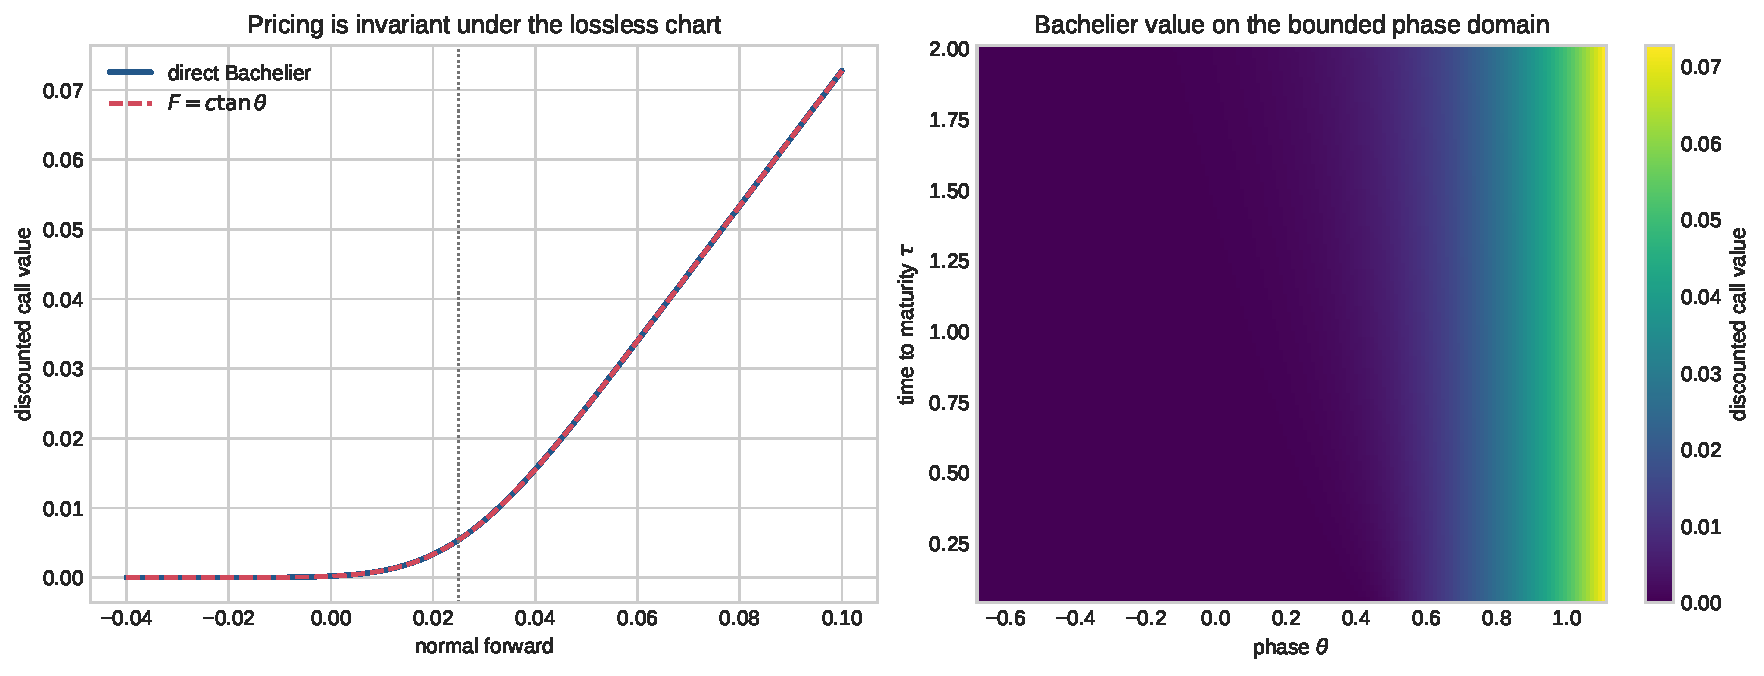
\includegraphics[width=1\linewidth,height=\textheight,keepaspectratio,alt={Left: direct and phase-coordinate Bachelier call curves coincide over negative and positive forwards. Right: the normal call value surface is plotted on the bounded phase interval across maturities.}]{figures/vector/f19_bachelier_coordinate_pricing.pdf}

}

\caption{\label{fig-bachelier-phase}Bachelier call prices in the scalar
and phase coordinates, and the value surface over phase and maturity.}

\end{figure}%

The benchmark behind Figure~\ref{fig-bachelier-phase} used \(c=0.05\),
\(K=0.025\), \(\sigma_N=0.0125\), \(\tau=1.25\), and \(D=0.97\). Across
\(401\) forward values from \(-0.04\) to \(0.10\), the maximum absolute
difference between Eq.~\ref{eq-bachelier-call} and
Eq.~\ref{eq-phase-bachelier} was \(2.78\times10^{-17}\). The calculation
includes negative forwards and both in- and out-of-the-money regimes.

\subsection{Delta, gamma, and hedge
conversion}\label{delta-gamma-and-hedge-conversion}

For the scalar normal call,

\begin{equation}\protect\phantomsection\label{eq-bachelier-greeks}{
\Delta_F
=\frac{\partial C_B}{\partial F}
=D(t,T)\Phi(d),
\qquad
\Gamma_F
=\frac{\partial^2C_B}{\partial F^2}
=D(t,T)\frac{\varphi(d)}{s}.
}\end{equation}

For a general value \(v(t,\theta)=V(t,c\tan\theta)\), inverse chain
rules give

\begin{equation}\protect\phantomsection\label{eq-delta-transform}{
\boxed{
V_x
=\frac{\cos^2\theta}{c}v_\theta,
}
}\end{equation}

and

\begin{equation}\protect\phantomsection\label{eq-gamma-transform}{
\boxed{
V_{xx}
=
\frac{
\cos^4\theta\,v_{\theta\theta}
-2\sin\theta\cos^3\theta\,v_\theta
}{c^2}.
}
}\end{equation}

The second term in Eq.~\ref{eq-gamma-transform} is a Hessian correction.
Omitting it is the deterministic analogue of omitting the Itô correction
in a transformed generator.

\begin{figure}[tbp]

\centering{

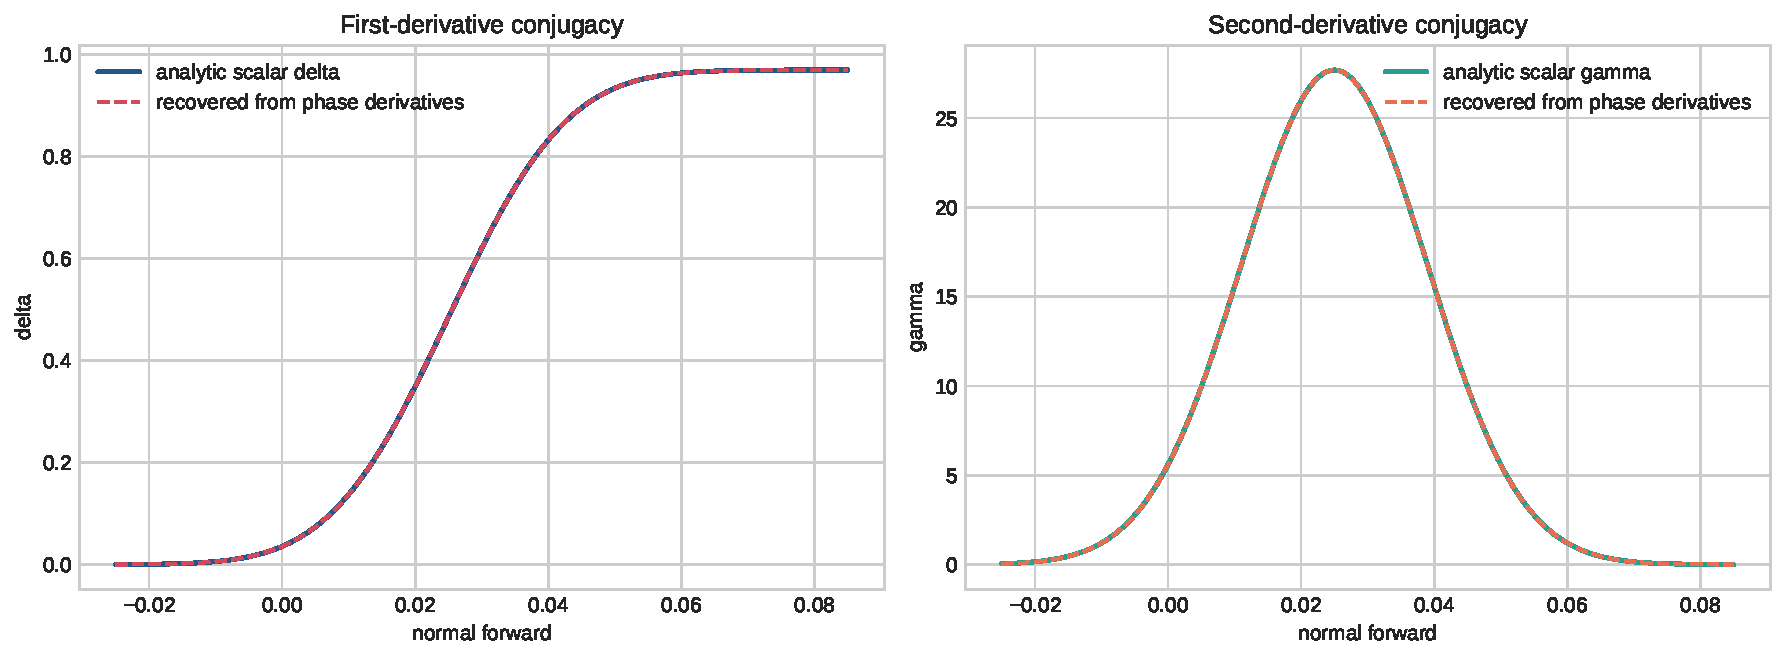
\includegraphics[width=1\linewidth,height=\textheight,keepaspectratio,alt={Two plots comparing analytic scalar Bachelier delta and gamma with the same Greeks reconstructed from finite-difference derivatives in phase. The paired curves overlap.}]{figures/vector/f20_greek_conjugacy.pdf}

}

\caption{\label{fig-greek-conjugacy}Bachelier delta and gamma recovered
from finite-difference phase derivatives.}

\end{figure}%

In Figure~\ref{fig-greek-conjugacy}, phase derivatives were computed by
centered differences with step \(7.5\times10^{-5}\) and converted by
Eq.~\ref{eq-delta-transform} and Eq.~\ref{eq-gamma-transform}. Against
independent analytic Greeks, the maximum absolute errors were
\(1.76\times10^{-8}\) for delta and \(5.81\times10^{-7}\) for gamma.

A self-financing hedge is coordinate invariant when the Jacobian is
handled correctly. If the hedge ratio is \(V_x\), using \(v_\theta\)
directly would be wrong by the factor \(d\theta/dx=\cos^2\theta/c\). The
auxiliary complex coordinate does not create another hedge instrument or
complete an otherwise incomplete market.

\subsection{Pricing-PDE verification}\label{pricing-pde-verification}

Under the driftless normal forward model and with discounting factored
out, the forward-maturity equation is

\begin{equation}\protect\phantomsection\label{eq-bachelier-forward-pde}{
V_\tau=\frac12\sigma_N^2V_{FF}.
}\end{equation}

The phase equation is

\begin{equation}\protect\phantomsection\label{eq-bachelier-phase-pde}{
v_\tau
=A(\theta)v_\theta
+\frac12B(\theta)^2v_{\theta\theta},
}\end{equation}

where

\[
A(\theta)
=-\frac{\sigma_N^2}{c^2}\sin\theta\cos^3\theta,
\qquad
B(\theta)=\frac{\sigma_N}{c}\cos^2\theta.
\]

\begin{figure}[tbp]

\centering{

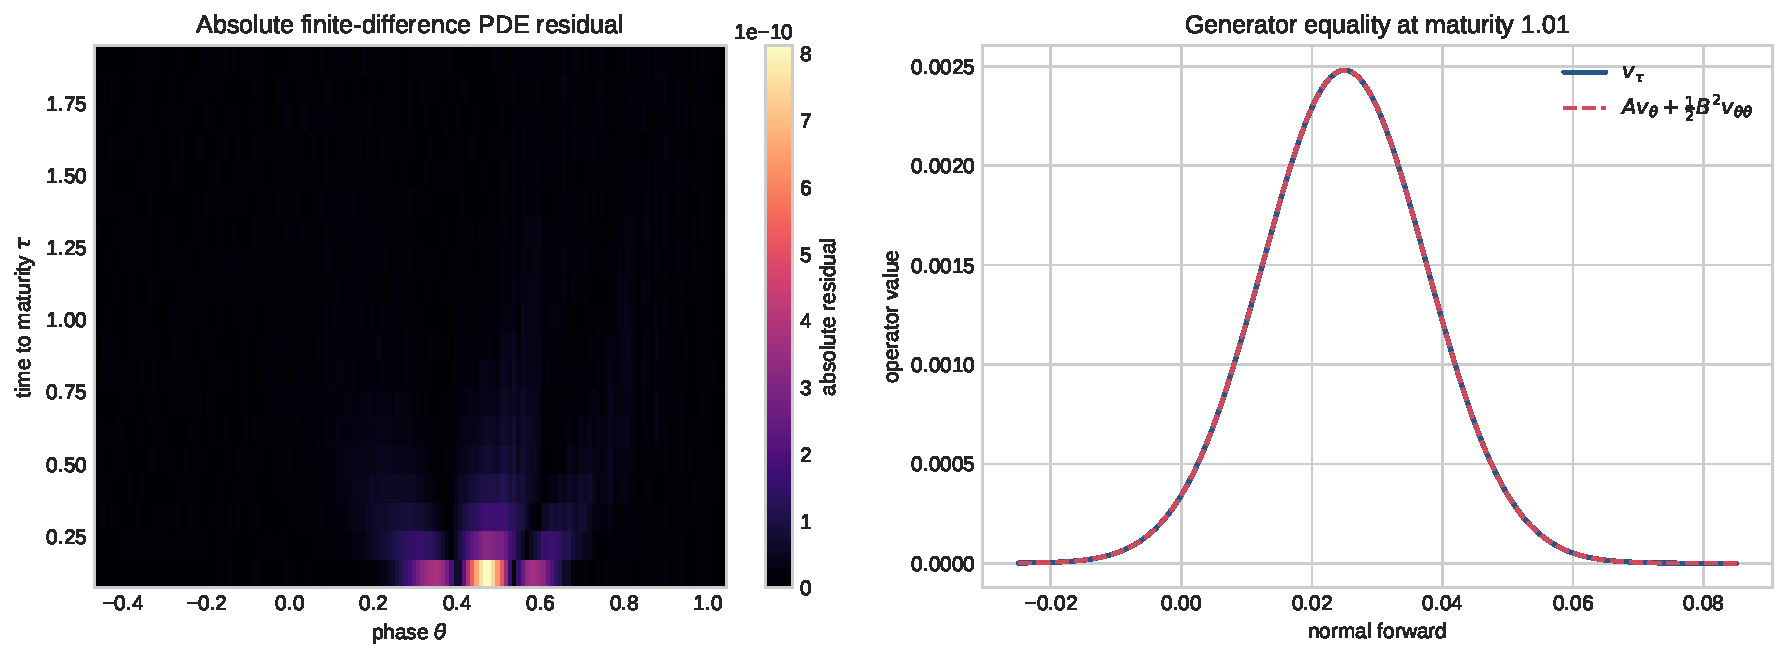
\includegraphics[width=1\linewidth,height=\textheight,keepaspectratio,alt={Left: heat map of the absolute residual between the maturity derivative and the transformed phase generator. Right: both operator values overlap across the forward range at a representative maturity.}]{figures/vector/f21_bachelier_pde_conjugacy.pdf}

}

\caption{\label{fig-bachelier-pde}Finite-difference verification of
Bachelier pricing-PDE conjugacy.}

\end{figure}%

Independent centered differences in phase and maturity were evaluated at
\(2{,}869\) grid points in Figure~\ref{fig-bachelier-pde}. The maximum
absolute residual was \(8.12\times10^{-10}\) and the RMS residual was
\(5.51\times10^{-11}\). The maximum relative residual was about
\(2.05\times10^{-3}\) only after dividing by operator values as small as
\(10^{-8}\); absolute residuals are the stable primary metric.

\subsection{Payoff regularity and compactified
boundaries}\label{payoff-regularity-and-compactified-boundaries}

The coordinate change does not smooth a payoff kink. A call kink at
\(x=K\) is moved to

\[
\theta_K=\arctan(K/c).
\]

For payoffs with polynomial growth, the transformed terminal condition
may diverge as \(\theta\to\pm\pi/2\) because
\(c\tan\theta\to\pm\infty\). Natural boundaries remove the need for a
probabilistic reflecting or absorbing condition, but a numerical method
on a truncated phase grid still needs consistent asymptotic treatment.
The concentration of grid points and the degeneracy \(B(\theta)\to0\)
can help or hurt depending on the payoff, basis, scale, and solver.

\section{Numerical methodology and evidence}\label{sec-numerics}

\subsection{Reproducible design}\label{reproducible-design}

The computational record is an executed Jupyter notebook generated by a
plain Python builder. It imports a tested mathematical module rather
than redefining the core transforms in disconnected cells. The
environment records Python 3.12, NumPy 2.5.1, SciPy 1.18.0, pandas
3.0.3, Matplotlib 3.11.1, and nbformat 5.10.4. The primary and
replication seed families are \(20260725\) and \(20360725\).

Comparisons use shared random streams when samplewise equality or strong
error is under study. Monte Carlo standard errors are retained. Every
publication figure is saved as vector PDF and raster PNG, and every
numerical assertion is saved as CSV or JSON. The notebook terminates
unless all \(22\) figures exist in both formats and its accuracy gates
pass.

The experiments are organized by evidentiary role:

\begin{itemize}
\tightlist
\item
  deterministic grids check exact reconstruction and inverse formulas;
\item
  independently advanced nonlinear schemes check phase SDE coefficients;
\item
  quadrature, simulation, and finite differences check the kernel,
  generator, semigroup, forward equation, and pricing PDE;
\item
  matched scalar/phase streams test estimator invariance; and
\item
  negative controls test dimension, path dependence, complex
  derivatives, winding, and numerical conditioning.
\end{itemize}

Simulation supports and stress-tests proofs; it does not establish a
theorem or a novelty claim.

\subsection{Nonlinear SDE convergence}\label{nonlinear-sde-convergence}

Euler--Maruyama, Milstein, and Stratonovich--Heun were advanced directly
from Eq.~\ref{eq-canonical-phase-sde} or
Eq.~\ref{eq-phase-stratonovich}. The exact arctangent update was used
only as a shared-path endpoint reference. With \(\mu=0.3\),
\(\sigma=0.8\), \(c=1.25\), \(T=1\), \(4{,}000\) paths, and step counts
\(32,\ldots,512\), the fitted strong slopes were:

\begin{longtable}[]{@{}
  >{\raggedright\arraybackslash}p{(\linewidth - 8\tabcolsep) * \real{0.2000}}
  >{\raggedleft\arraybackslash}p{(\linewidth - 8\tabcolsep) * \real{0.2000}}
  >{\raggedleft\arraybackslash}p{(\linewidth - 8\tabcolsep) * \real{0.2000}}
  >{\raggedleft\arraybackslash}p{(\linewidth - 8\tabcolsep) * \real{0.2000}}
  >{\raggedleft\arraybackslash}p{(\linewidth - 8\tabcolsep) * \real{0.2000}}@{}}
\caption{Shared-path strong-convergence
estimates.}\label{tbl-strong-convergence}\tabularnewline
\toprule\noalign{}
\begin{minipage}[b]{\linewidth}\raggedright
Method
\end{minipage} & \begin{minipage}[b]{\linewidth}\raggedleft
Base-seed slope
\end{minipage} & \begin{minipage}[b]{\linewidth}\raggedleft
Replication slope
\end{minipage} & \begin{minipage}[b]{\linewidth}\raggedleft
Base RMSE at 512 steps
\end{minipage} & \begin{minipage}[b]{\linewidth}\raggedleft
Replication RMSE
\end{minipage} \\
\midrule\noalign{}
\endfirsthead
\toprule\noalign{}
\begin{minipage}[b]{\linewidth}\raggedright
Method
\end{minipage} & \begin{minipage}[b]{\linewidth}\raggedleft
Base-seed slope
\end{minipage} & \begin{minipage}[b]{\linewidth}\raggedleft
Replication slope
\end{minipage} & \begin{minipage}[b]{\linewidth}\raggedleft
Base RMSE at 512 steps
\end{minipage} & \begin{minipage}[b]{\linewidth}\raggedleft
Replication RMSE
\end{minipage} \\
\midrule\noalign{}
\endhead
\bottomrule\noalign{}
\endlastfoot
Euler--Maruyama & 0.493 & 0.510 & \(5.65\times10^{-3}\) &
\(5.45\times10^{-3}\) \\
Milstein & 1.006 & 1.011 & \(3.46\times10^{-4}\) &
\(3.51\times10^{-4}\) \\
Stratonovich--Heun & 1.001 & 1.000 & \(2.69\times10^{-4}\) &
\(2.71\times10^{-4}\) \\
\end{longtable}

The expected orders \(1/2\) and \(1\) appear in two independent seed
families, as visualized in Figure~\ref{fig-phase-convergence}. This is a
non-circular check of the derived coefficients. The exact step remains
merely the known Gaussian step conjugated by a known inverse; it is not
a general exact-simulation algorithm in the sense of (Beskos and Roberts
2005).

\subsection{Heat-equation compactification
benchmark}\label{heat-equation-compactification-benchmark}

To isolate numerical effects from financial payoff singularities, the
notebook also solved

\begin{equation}\protect\phantomsection\label{eq-heat-benchmark}{
\partial_tu=\frac12\partial_{xx}u,
\qquad
u(0,x)=e^{-x^2},
}\end{equation}

at \(T=0.35\), with physical truncation \([-8,8]\). Direct-\(x\) and
\(x=c\tan\theta\) grids used matched total point counts, and errors were
compared on the common region \(|x|\le4\).

\begin{longtable}[]{@{}
  >{\raggedright\arraybackslash}p{(\linewidth - 10\tabcolsep) * \real{0.1667}}
  >{\raggedleft\arraybackslash}p{(\linewidth - 10\tabcolsep) * \real{0.1667}}
  >{\raggedleft\arraybackslash}p{(\linewidth - 10\tabcolsep) * \real{0.1667}}
  >{\raggedleft\arraybackslash}p{(\linewidth - 10\tabcolsep) * \real{0.1667}}
  >{\raggedleft\arraybackslash}p{(\linewidth - 10\tabcolsep) * \real{0.1667}}
  >{\raggedleft\arraybackslash}p{(\linewidth - 10\tabcolsep) * \real{0.1667}}@{}}
\caption{Matched-grid compactification benchmark on
\(|x|\le4\).}\label{tbl-pde-benchmark}\tabularnewline
\toprule\noalign{}
\begin{minipage}[b]{\linewidth}\raggedright
Coordinate
\end{minipage} & \begin{minipage}[b]{\linewidth}\raggedleft
\(c\)
\end{minipage} & \begin{minipage}[b]{\linewidth}\raggedleft
Points
\end{minipage} & \begin{minipage}[b]{\linewidth}\raggedleft
Maximum error
\end{minipage} & \begin{minipage}[b]{\linewidth}\raggedleft
RMS error
\end{minipage} & \begin{minipage}[b]{\linewidth}\raggedleft
Condition proxy
\end{minipage} \\
\midrule\noalign{}
\endfirsthead
\toprule\noalign{}
\begin{minipage}[b]{\linewidth}\raggedright
Coordinate
\end{minipage} & \begin{minipage}[b]{\linewidth}\raggedleft
\(c\)
\end{minipage} & \begin{minipage}[b]{\linewidth}\raggedleft
Points
\end{minipage} & \begin{minipage}[b]{\linewidth}\raggedleft
Maximum error
\end{minipage} & \begin{minipage}[b]{\linewidth}\raggedleft
RMS error
\end{minipage} & \begin{minipage}[b]{\linewidth}\raggedleft
Condition proxy
\end{minipage} \\
\midrule\noalign{}
\endhead
\bottomrule\noalign{}
\endlastfoot
direct \(x\) & --- & 161 & \(4.65\times10^{-4}\) & \(1.78\times10^{-4}\)
& 1.70 \\
phase & 0.5 & 161 & \(1.99\times10^{-4}\) & \(6.04\times10^{-5}\) &
78.8 \\
phase & 1.0 & 161 & \(5.98\times10^{-5}\) & \(2.28\times10^{-5}\) &
22.1 \\
phase & 2.0 & 161 & \(4.07\times10^{-5}\) & \(2.55\times10^{-5}\) &
7.30 \\
\end{longtable}

\begin{figure}[tbp]

\centering{

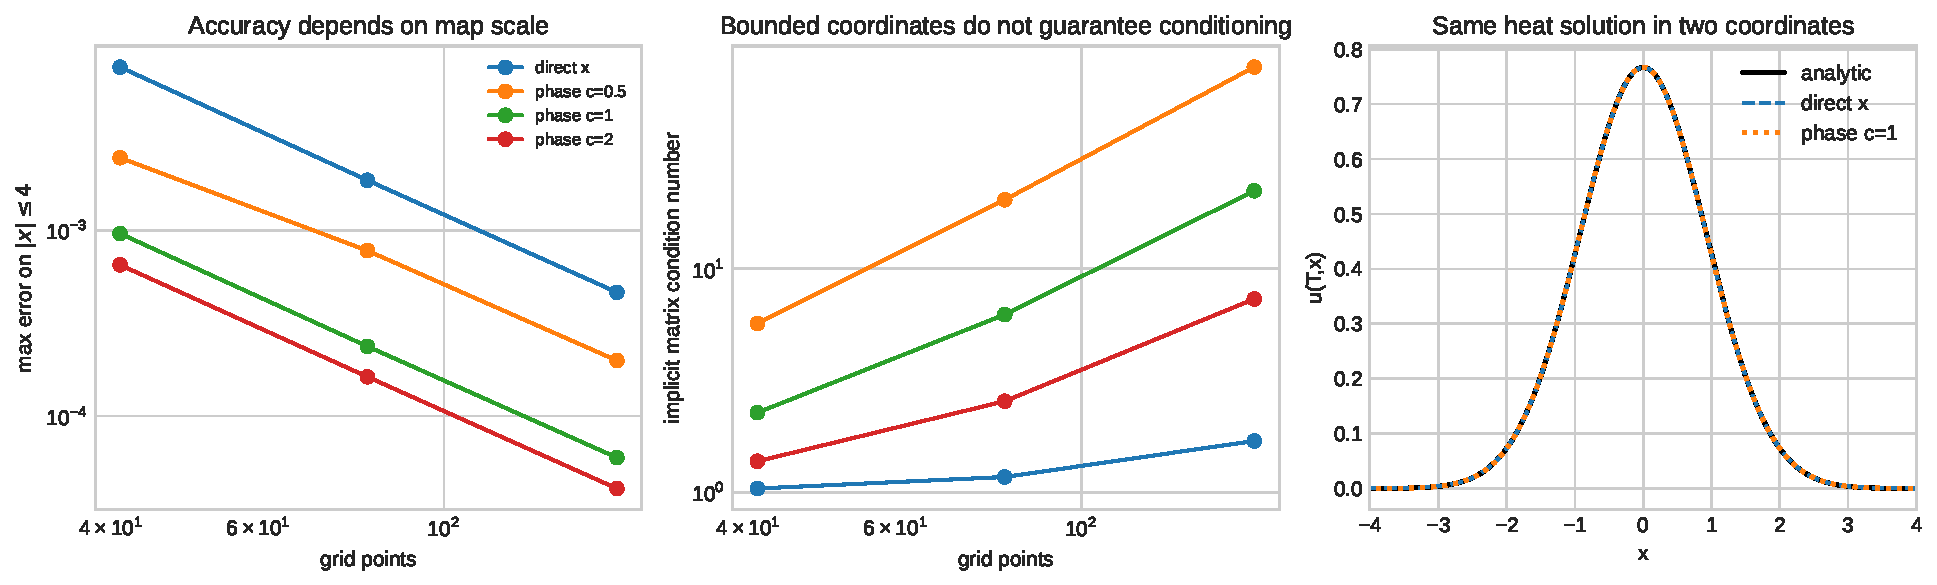
\includegraphics[width=1\linewidth,height=\textheight,keepaspectratio,alt={Three panels compare maximum central-region error, a matrix-condition proxy, and numerical solutions for direct and phase grids across several resolutions and map scales.}]{figures/vector/f16_pde_compactification.pdf}

}

\caption{\label{fig-pde-compactification}Accuracy and conditioning
trade-offs for direct and arctangent-compactified heat-equation grids.}

\end{figure}%

At \(161\) points, the best mapped maximum error in
Table~\ref{tbl-pde-benchmark} was about \(11.4\) times smaller than the
direct-grid error, but even the best-conditioned mapped case had a
condition proxy about \(4.3\) times larger. At \(c=0.5\), conditioning
deteriorated far more. The qualified conclusion agrees with the
mapped-domain literature (Grosch and Orszag 1977; Boyd 1987):
compactification can reallocate resolution, but its value is scale-,
solution-, discretization-, and metric-dependent.

\subsection{Monte Carlo and quasi-Monte Carlo
invariance}\label{monte-carlo-and-quasi-monte-carlo-invariance}

For any terminal payoff \(g\),

\begin{equation}\protect\phantomsection\label{eq-payoff-sample-invariance}{
g(X_T)=g(c\tan\theta_T)
}\end{equation}

sample by sample. Consequently, if the same random stream is used,

\begin{equation}\protect\phantomsection\label{eq-estimator-invariance}{
\widehat V_X=\widehat V_\theta,
\qquad
\widehat{\operatorname{Var}}_X
=\widehat{\operatorname{Var}}_\theta.
}\end{equation}

\begin{figure}[tbp]

\centering{

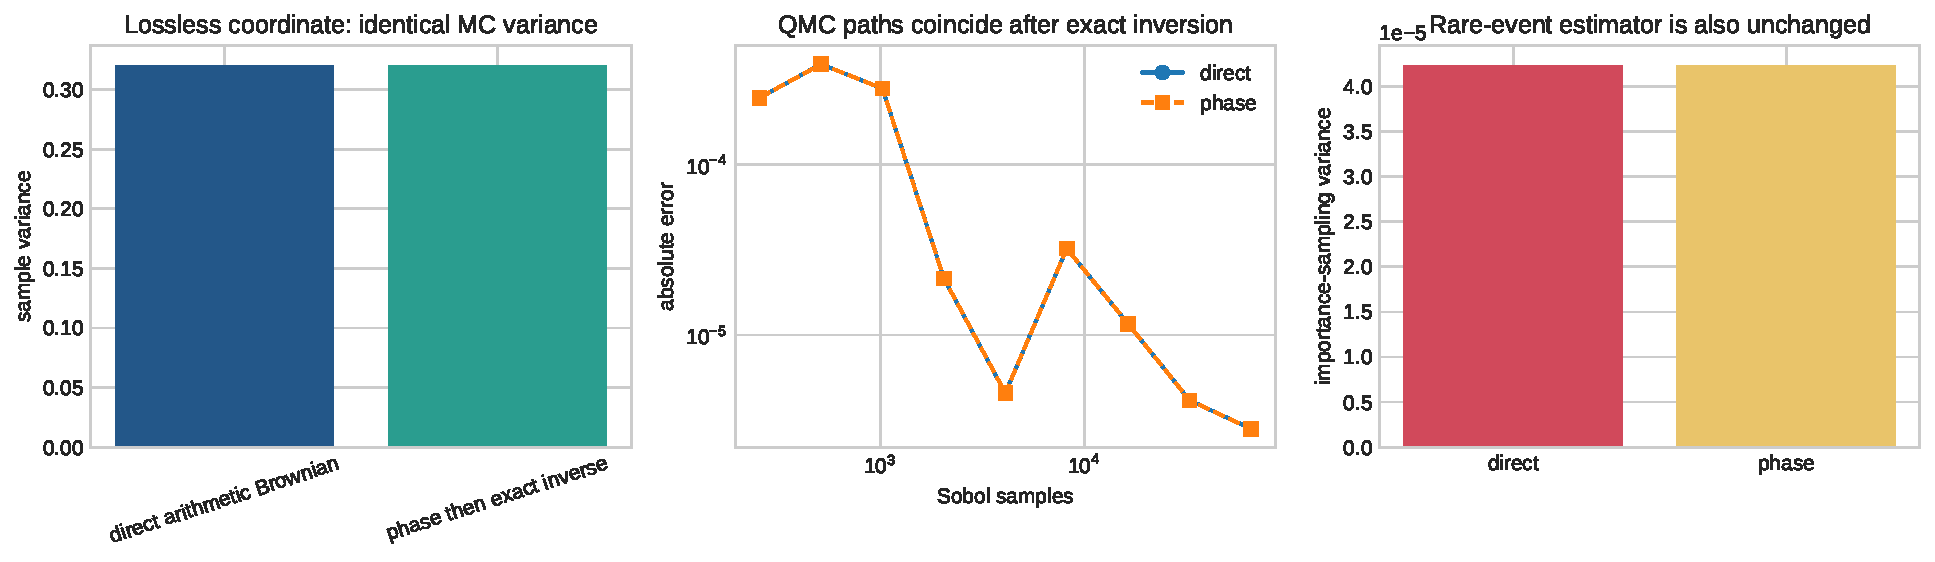
\includegraphics[width=1\linewidth,height=\textheight,keepaspectratio,alt={Three panels show identical direct and phase sample variance for ordinary Monte Carlo, coincident quasi-Monte Carlo errors, and identical importance-sampling variance.}]{figures/vector/f17_monte_carlo_equivalence.pdf}

}

\caption{\label{fig-mc-equivalence}Ordinary Monte Carlo, scrambled
Sobol, and importance-sampling comparisons under the exact phase round
trip.}

\end{figure}%

In Figure~\ref{fig-mc-equivalence}, the direct and phase
Bachelier-payoff estimators both returned \(0.363588299584\), sample
variance \(0.320662659809\), and standard error \(0.00110599773\). State
and payoff discrepancies were at most \(1.78\times10^{-15}\). Scrambled
Sobol estimates and an importance-sampled rare-event estimate also
agreed. The phase route retains one random dimension and adds an
arctangent/tangent round trip. Variance reduction could arise only from
another algorithmic change---such as a new proposal, control variate,
smoothing, stratification, or basis---not from exact relabeling alone.

\subsection{Path dependence and multifactor
controls}\label{path-dependence-and-multifactor-controls}

A terminal phase is sufficient for a terminal one-factor payoff because
it determines \(X_T\). It is not sufficient for a generic path
functional. To make the distinction exact, the notebook simulated
\(28{,}000\) Brownian bridges pinned at the same terminal forward. Their
terminal phase spread was \(2.78\times10^{-16}\), yet their time-average
forward had standard deviation \(0.00427\) and \(1\%\)--\(99\%\)
quantiles \(0.0101\) and \(0.0300\).

A second control simulated a nonsingular correlated two-factor Gaussian
law. Its smallest covariance eigenvalue was \(0.654\), its determinant
was \(0.879\), and its rank was two. No smooth one-dimensional phase
chart can be a diffeomorphism onto an open two-dimensional support.

\begin{figure}[tbp]

\centering{

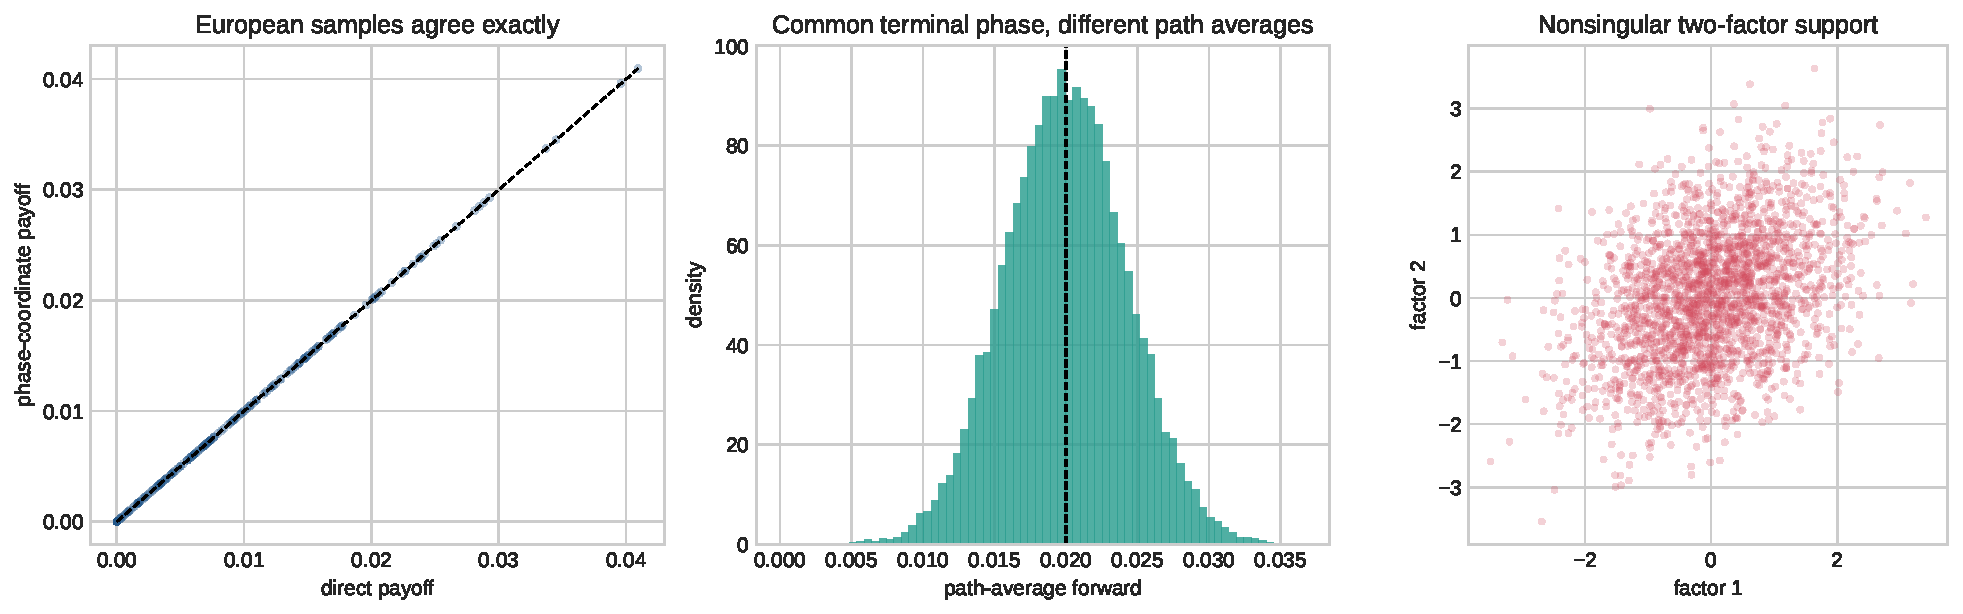
\includegraphics[width=1\linewidth,height=\textheight,keepaspectratio,alt={Left: direct and phase European payoff samples lie on the diagonal. Center: pinned Brownian bridges share a terminal phase but have dispersed path averages. Right: a correlated two-factor Gaussian cloud has planar support.}]{figures/vector/f22_financial_scope_controls.pdf}

}

\caption{\label{fig-financial-controls}Financial scope controls for
European payoff invariance, pinned-path dependence, and two-factor
support.}

\end{figure}%

Figure~\ref{fig-financial-controls} separates three claims:

\begin{longtable}[]{@{}
  >{\raggedright\arraybackslash}p{(\linewidth - 2\tabcolsep) * \real{0.5000}}
  >{\raggedright\arraybackslash}p{(\linewidth - 2\tabcolsep) * \real{0.5000}}@{}}
\caption{Financial scope
controls.}\label{tbl-financial-controls}\tabularnewline
\toprule\noalign{}
\begin{minipage}[b]{\linewidth}\raggedright
Claim
\end{minipage} & \begin{minipage}[b]{\linewidth}\raggedright
Result
\end{minipage} \\
\midrule\noalign{}
\endfirsthead
\toprule\noalign{}
\begin{minipage}[b]{\linewidth}\raggedright
Claim
\end{minipage} & \begin{minipage}[b]{\linewidth}\raggedright
Result
\end{minipage} \\
\midrule\noalign{}
\endhead
\bottomrule\noalign{}
\endlastfoot
Exact phase changes a European payoff sample & Refuted; maximum
difference \(1.39\times10^{-17}\) \\
Terminal phase determines a path average & Refuted by pinned bridges \\
One smooth phase losslessly represents a nonsingular two-factor law &
Refuted by covariance rank two \\
\end{longtable}

The full phase \emph{path} is equivalent to the full scalar path. The
negative result concerns replacing path history by the terminal phase
alone.

\section{Stochastic dimension and vector geometry}\label{sec-vector}

\subsection{Tangent, normal, and instantaneous
covariance}\label{tangent-normal-and-instantaneous-covariance}

For a \(C^2\) phase curve \(F:I\to\mathbb C\), the complex derivative
\(F'(\theta)\) is a tangent vector under \(\mathbb C\simeq\mathbb R^2\),
and \(iF'(\theta)\) is its quarter-turned normal. If

\[
d\theta_t=m(\theta_t)dt+s(\theta_t)dW_t,
\]

then the real Cartesian diffusion vector of \(Z_t=Z_0F(\theta_t)\) is

\[
q(\theta)
=
s(\theta)
\begin{pmatrix}
\operatorname{Re}\{Z_0F'(\theta)\}\\
\operatorname{Im}\{Z_0F'(\theta)\}
\end{pmatrix}.
\]

Its instantaneous covariance density is the outer product

\begin{equation}\protect\phantomsection\label{eq-rank-one-covariance}{
\boxed{
\Sigma(\theta)=q(\theta)q(\theta)^\mathsf T,
\qquad
\operatorname{rank}\Sigma(\theta)\le1.
}
}\end{equation}

Multiplication by \(i\) rotates \(q\) but does not supply an independent
increment. To obtain independent tangential and normal Brownian forcing,
the model needs another driver or an explicitly higher-rank diffusion
matrix.

\begin{figure}[tbp]

\centering{

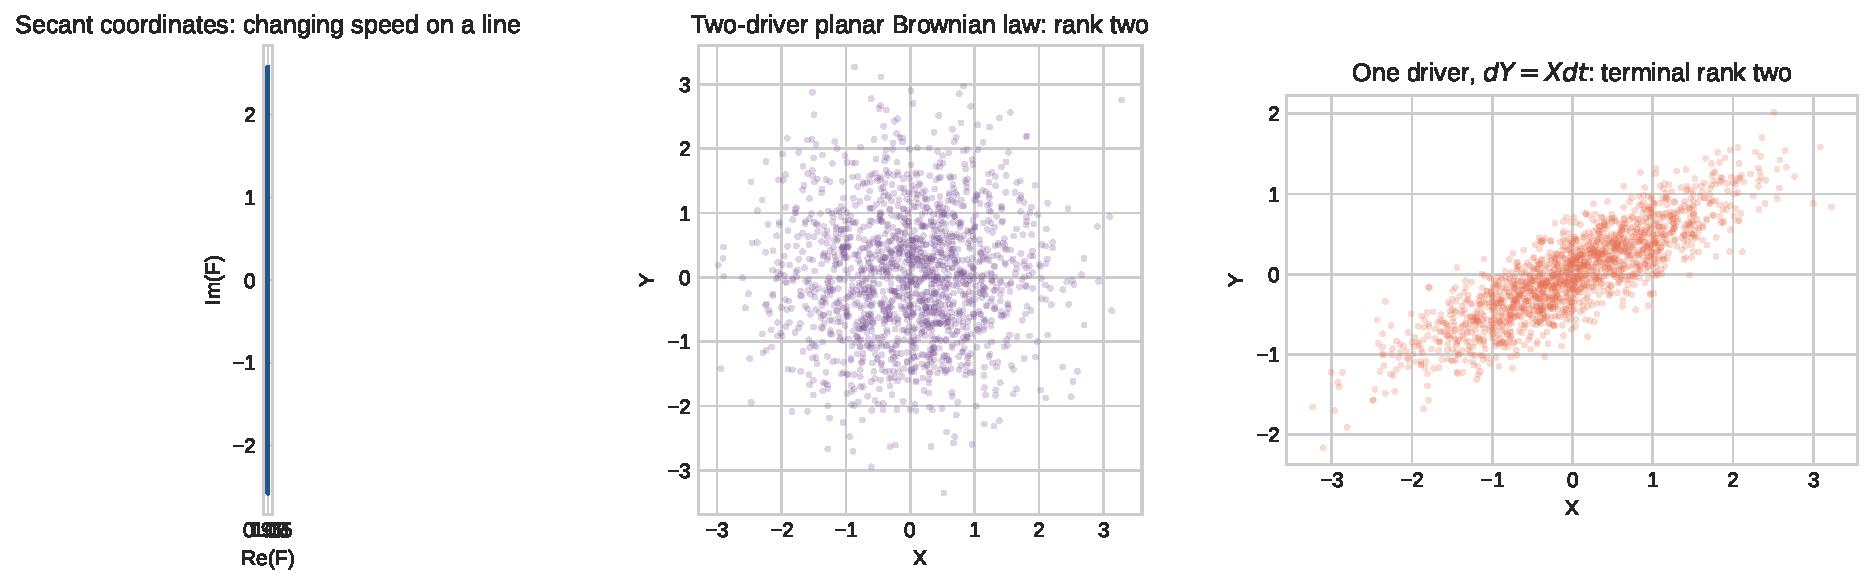
\includegraphics[width=1\linewidth,height=\textheight,keepaspectratio,alt={Panels show tangent and normal vectors on the phase curve, the eigenvalues of its rank-one covariance, and rank-two planar Brownian and hypoelliptic terminal covariance controls.}]{figures/vector/f14_vector_geometry_and_controls.pdf}

}

\caption{\label{fig-vector-controls}Curve tangents and normals,
instantaneous rank-one covariance, and higher-dimensional negative
controls.}

\end{figure}%

\subsection{Four notions of dimension}\label{four-notions-of-dimension}

The phrase ``one-dimensional noise'' can refer to different objects. It
is important to distinguish:

\begin{enumerate}
\def\labelenumi{\arabic{enumi}.}
\tightlist
\item
  the number of Brownian drivers;
\item
  the rank of the instantaneous diffusion covariance;
\item
  the dimension of the fixed-time support; and
\item
  the dimension of a sufficient Markov state.
\end{enumerate}

For the affine process classified here, all four relevant state notions
are one-dimensional. This is not a universal implication of having one
driver. For example,

\begin{equation}\protect\phantomsection\label{eq-integrated-brownian}{
dX_t=dW_t,\qquad dY_t=X_t\,dt
}\end{equation}

has one Brownian driver and instantaneous covariance rank one, but

\begin{equation}\protect\phantomsection\label{eq-hypoelliptic-covariance}{
\operatorname{Cov}(X_1,Y_1)
=
\begin{pmatrix}
1&1/2\\
1/2&1/3
\end{pmatrix},
\qquad
\det=\frac1{12}>0.
}\end{equation}

The drift propagates noise into a second state direction. This
elementary hypoelliptic example reflects the broader support and bracket
phenomena studied by Stroock--Varadhan and Hörmander (Stroock and
Varadhan 1972; Hörmander 1967). The notebook's empirical covariance was
within \(8.55\times10^{-3}\) of Eq.~\ref{eq-hypoelliptic-covariance} and
had rank two, as did a planar Brownian control.

Thus neither shortcut is valid:

\[
\text{one driver}\not\Rightarrow
\text{one-dimensional terminal support},
\]

and

\[
\text{complex notation}\not\Rightarrow
\text{two stochastic dimensions}.
\]

\subsection{What vector geometry does
contribute}\label{what-vector-geometry-does-contribute}

The complex chart provides concise tangent-normal bookkeeping. In more
general curve-valued models it can organize projections, curvature
drift, constraint error, and invariant-preserving updates. In the
present additive case, however, the secant curve has zero curvature and
all tangents are parallel. The geometry explains the model's rank-one
structure; it does not enlarge it.

The rigidity theorems convert coefficient matching into geometry:

\begin{itemize}
\tightlist
\item
  constant additive noise requires constant tangent direction, hence a
  line;
\item
  constant multiplicative noise requires constant logarithmic tangent
  \(F'/F\), hence a logarithmic spiral; and
\item
  a general polar curve induces state-dependent complex coefficients.
\end{itemize}

This is a useful coordinate interface to existing vector stochastic
calculus, not a new vector calculus.

\section{Complex differentiation and analytic
implications}\label{sec-complex-analysis}

\subsection{A curve determines only tangential
derivatives}\label{a-curve-determines-only-tangential-derivatives}

A complex derivative at an interior point of an open subset of
\(\mathbb C\) requires compatible limits from all directions. Data
restricted to the one-dimensional state curve determine only a
tangential derivative.

On the canonical line \(\{1+iy:y\in\mathbb R\}\), consider

\[
H_0(z)=0,\qquad
H_1(z)=\operatorname{Re}z-1.
\]

Both functions vanish on the entire state line, yet their normal
derivatives are \(0\) and \(1\). Hence the stochastic state data do not
select a unique off-curve extension, much less a unique holomorphic
extension.

\subsection{Wirtinger calculus}\label{wirtinger-calculus}

For a real-differentiable \(H(z,\bar z)\), define

\[
H_z=\frac12(H_x-iH_y),
\qquad
H_{\bar z}=\frac12(H_x+iH_y).
\]

Along \(z=F(\theta)\),

\begin{equation}\protect\phantomsection\label{eq-wirtinger-pullback}{
\frac{d}{d\theta}
H(F(\theta),\overline{F(\theta)})
=
H_zF'(\theta)+H_{\bar z}\overline{F'(\theta)}.
}\end{equation}

This compactly packages two real derivatives (Brandwood 1983). It
becomes holomorphic calculus only when \(H_{\bar z}=0\) on an open
domain. The notebook checked Eq.~\ref{eq-wirtinger-pullback} for
\(H(z,\bar z)=|z|^2\) to \(3.55\times10^{-15}\), while the two
extensions above agreed exactly on the curve and retained different
normal derivatives.

\subsection{Complex-step differentiation and transform
methods}\label{complex-step-differentiation-and-transform-methods}

For a real function with a suitable analytic extension,

\[
f'(x)\approx\frac{\operatorname{Im}f(x+ih)}h
\]

can avoid subtractive cancellation (Squire and Trapp 1998). That
advantage comes from the analytic extension and the complex-step
algorithm. The phase chart does not supply off-curve values or guarantee
analyticity of a payoff.

Similarly, complex methods in models such as Heston and in Fourier
pricing derive their power from characteristic functions, contour
choices, damping, and transform inversion (Heston 1993; Carr and Madan
1999). Writing a real Bachelier state as \(\sec\theta e^{i\theta}\)
neither replaces nor automatically improves those methods.

\begin{figure}[tbp]

\centering{

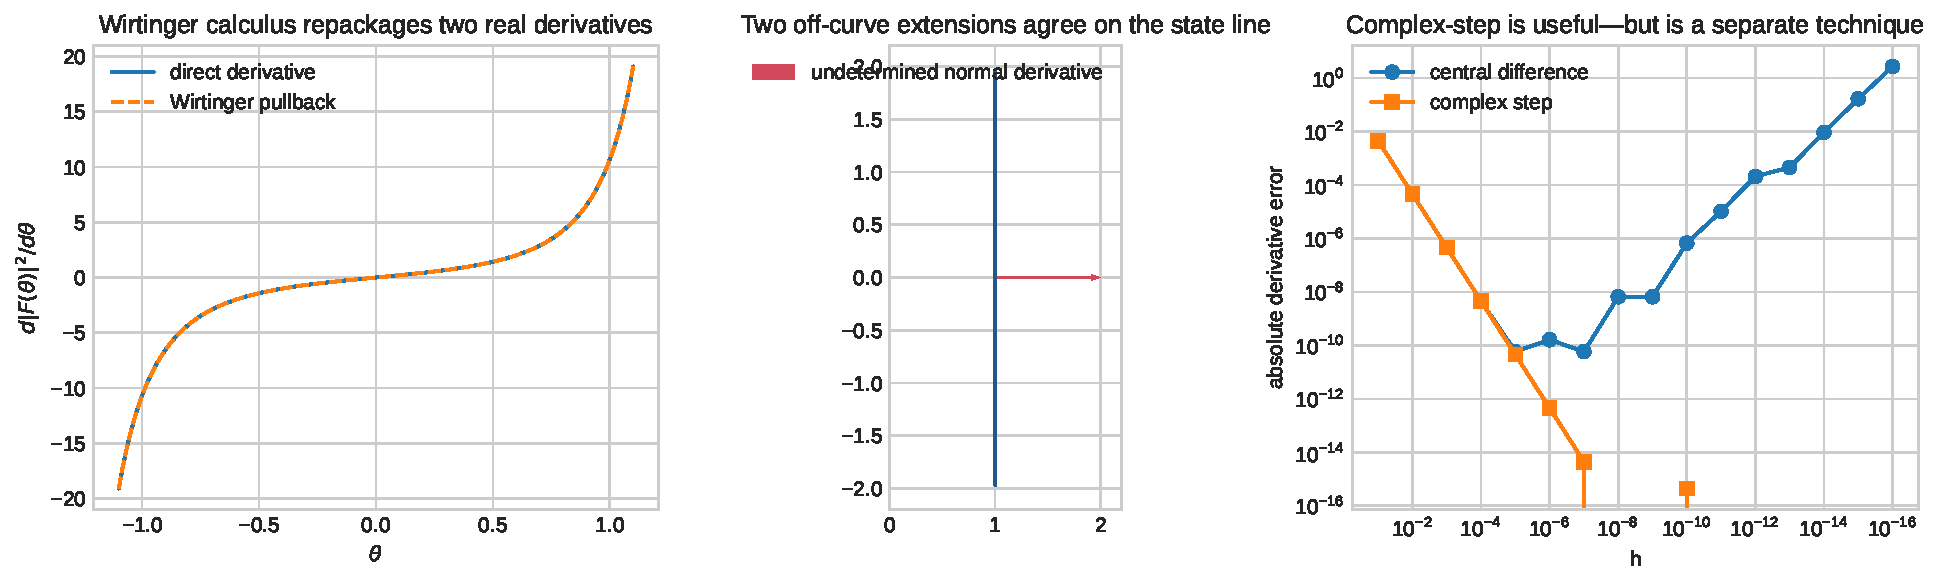
\includegraphics[width=1\linewidth,height=\textheight,keepaspectratio,alt={Panels show two extensions agreeing on the state curve but differing normally, numerical verification of a Wirtinger pullback identity, and complex-step versus finite-difference error for an analytic function.}]{figures/vector/f15_complex_derivative_limits.pdf}

}

\caption{\label{fig-complex-derivative-limits}Off-curve derivative
nonuniqueness, Wirtinger pullback, and the separate complex-step
benchmark.}

\end{figure}%

Figure~\ref{fig-complex-derivative-limits} summarizes the boundary:
complex notation is valuable for organization and for methods whose own
analytic assumptions hold; Euler form alone creates no holomorphic
derivative.

\section{Computational implications and research
agenda}\label{sec-research-agenda}

\subsection{What is analytically
gained}\label{what-is-analytically-gained}

The phase chart supplies exact formulas for an already solvable affine
diffusion:

\begin{itemize}
\tightlist
\item
  a bounded state coordinate and explicit inverse;
\item
  an autonomous nonlinear SDE;
\item
  an exact transition density and update;
\item
  natural-boundary behavior;
\item
  a conjugate generator and pricing PDE;
\item
  exact transformed Bachelier values and Greeks; and
\item
  group and rigidity interpretations.
\end{itemize}

This package can simplify reasoning when a bounded chart, polar
geometry, or state-dependent grid is desirable. It also creates a
demanding but exactly solvable benchmark for nonlinear SDE schemes.

It does \textbf{not} turn a previously unsolved stochastic problem into
a closed form. Every canonical analytic formula is inherited from
arithmetic Brownian motion through a diffeomorphism. An invertible
coordinate change preserves information and exact option values. Any
computational improvement must enter through the interaction between the
coordinate and an additional numerical choice.

\subsection{Qualified opportunities}\label{qualified-opportunities}

\subsubsection{Adaptive and spectral PDE
methods}\label{adaptive-and-spectral-pde-methods}

The map scale \(c\) provides a principled way to concentrate resolution
near a region of financial interest while retaining an unbounded
physical domain. Rational spectral bases induced by related maps have
established theory (Boyd 1987). A useful next result would optimize
\(c\) jointly with payoff regularity, tail asymptotics, grid order, and
a conditioning constraint, rather than report a single favorable error.

\subsubsection{Structure-preserving phase
integration}\label{structure-preserving-phase-integration}

Exact transformed steps preserve the natural interval, and exact Cayley
steps preserve unit modulus. For models without an exact inverse,
geometric and symmetry-adapted schemes may exploit the same invariants
(Malham and Wiese 2008; De Vecchi et al. 2019). A rigorous extension
would compare weak and strong error at matched computational cost while
measuring constraint defect separately.

\subsubsection{Financial normal-model
calculations}\label{financial-normal-model-calculations}

The phase can be useful when normal factors range over wide positive and
negative values and a bounded PDE coordinate is operationally
convenient. It does not change calibration targets or risk measures.
Empirical work would need to compare stability of calibration,
extrapolation, and Greeks under specified market data, boundary
conventions, and regularization.

\subsubsection{Higher-dimensional
geometry}\label{higher-dimensional-geometry}

Multifactor extensions should retain their actual dimension. Candidate
coordinates include products of one-dimensional charts, projective or
spherical charts with multiple phases, and manifold methods whose
diffusion rank is explicit. Hörmander brackets and support must be
analyzed rather than inferred from driver count. A single phase should
be used only after a sufficient-statistic or invariant-manifold theorem
proves losslessness.

\subsubsection{Path-dependent claims}\label{path-dependent-claims}

The terminal phase cannot encode a Brownian bridge. For Asian, barrier,
and early-exercise claims, legitimate approaches include augmenting the
Markov state with running integrals or extrema, simulating the full
phase path, or using regression and dynamic programming (Longstaff and
Schwartz 2001; Zhang 2003). The phase may still serve as one coordinate
of that expanded state.

\subsubsection{Beyond affine and log-affine
rigidity}\label{beyond-affine-and-log-affine-rigidity}

For a prescribed smooth radius \(r(\theta)\) and phase diffusion,
Eq.~\ref{eq-general-curve-ito} constructs a state-dependent complex SDE.
A broader classification could ask which drift-diffusion families
preserve selected curves or admit global polar charts across zeros. Such
work belongs to stochastic differential geometry and should not be
inferred from the affine line alone.

\subsection{Decision map}\label{decision-map}

\begin{figure}[tbp]

\centering{

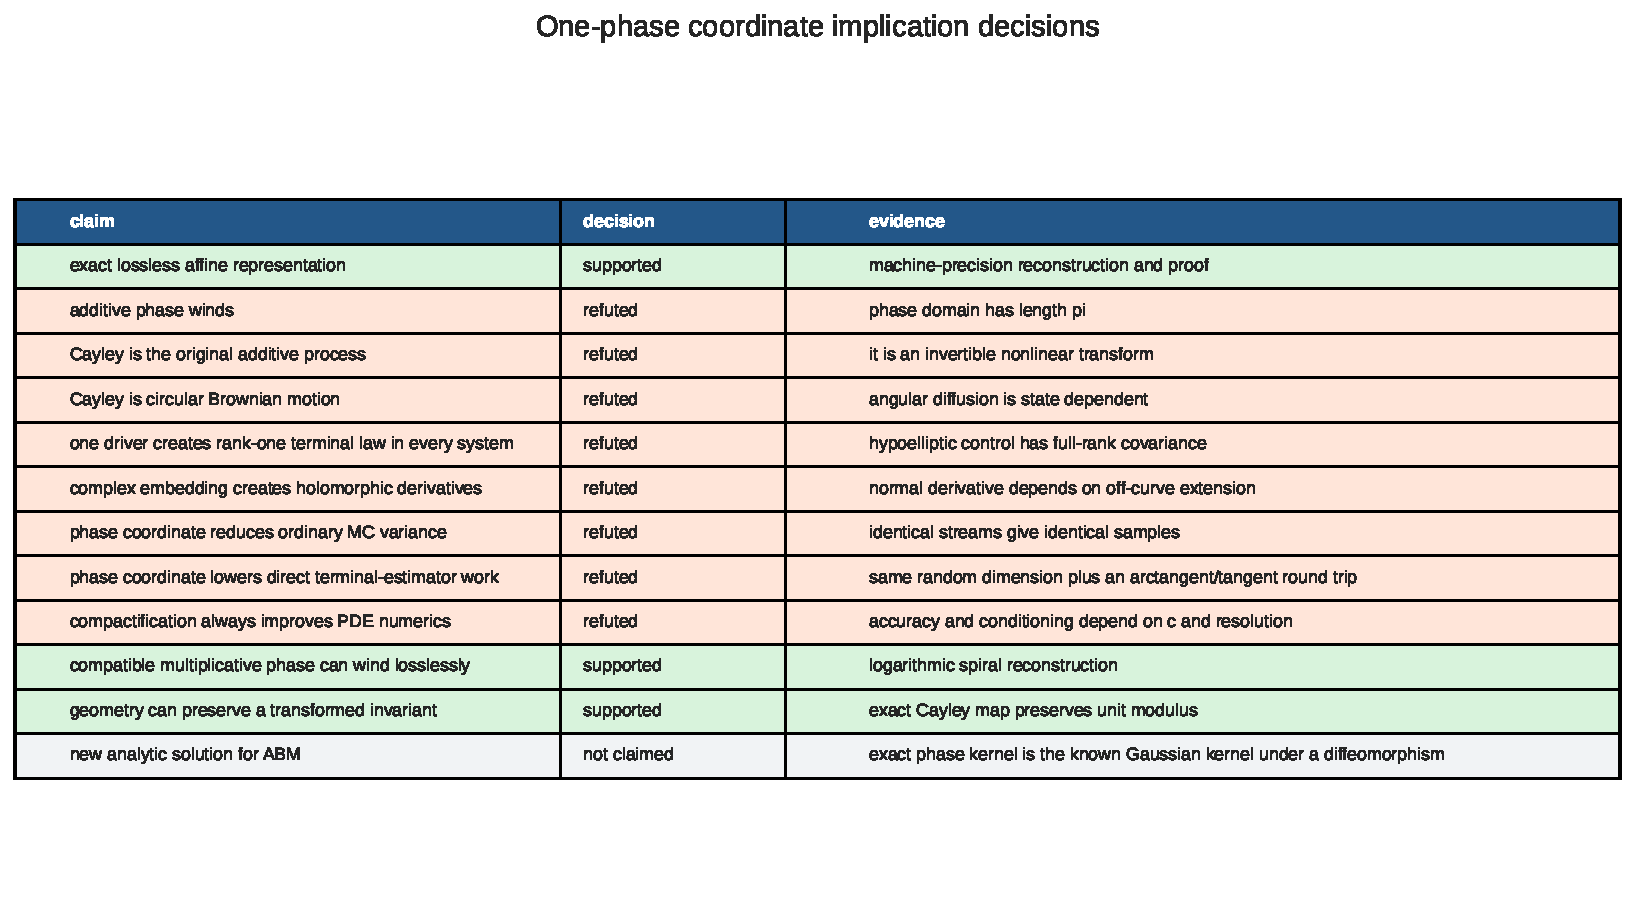
\includegraphics[width=1\linewidth,height=\textheight,keepaspectratio,alt={A color-coded decision table marking exact affine representation and compatible spiral winding as supported, and rejecting circular Brownian, added stochastic dimension, generic variance reduction, holomorphic structure, and universal PDE improvement claims.}]{figures/vector/f18_evidence_decisions.pdf}

}

\caption{\label{fig-evidence-decisions}Evidence-based decisions for the
principal claims and negative controls.}

\end{figure}%

The decision map in Figure~\ref{fig-evidence-decisions} enforces a
conservative interpretation. Exactness, lossless reconstruction, the
affine classification, and conjugate pricing are supported. Automatic
variance reduction, ordinary circular Brownian behavior, added
dimension, universal conditioning improvement, and new complex
analyticity are not.

\section{Limitations}\label{sec-limitations}

The scope of the results is deliberately narrow.

\begin{enumerate}
\def\labelenumi{\arabic{enumi}.}
\tightlist
\item
  \textbf{One real driver and constant affine coefficients.} The global
  iff theorem concerns \(Z_0+at+bW_t\). State-dependent coefficients,
  jumps, multiple Brownian drivers, and random coefficients require new
  support and regularity arguments.
\item
  \textbf{Genuine polar phase.} Pathological measurable encodings of
  higher-dimensional data into one real number are irrelevant to the
  smooth, geometric, Itô-compatible problem.
\item
  \textbf{Nonvanishing reference geometry.} The main normalization
  assumes \(Z_0\ne0\) and the eligible line misses the origin. Charts
  across zeros need stopping times or multiple coordinate patches.
\item
  \textbf{No unlimited additive winding.} The additive phase interval
  has length \(\pi\). Unlimited winding belongs to the compatible
  multiplicative spiral, which is a different process.
\item
  \textbf{Normal-model financial scope.} Arithmetic Brownian levels can
  become negative. The model is not a universal equity-price model, and
  the complex coordinate is not traded.
\item
  \textbf{Classical smooth pricing.} The PDE derivation assumes
  sufficient regularity. Viscosity, weak, or distributional formulations
  are needed for nonsmooth coefficients and payoffs, although
  conditional-expectation invariance remains immediate when integrable.
\item
  \textbf{Finite numerical audit.} Convergence slopes, residuals, and
  compactification errors are finite-resolution measurements. Only the
  algebraic identities are exact to mathematical precision.
\item
  \textbf{No universal computational advantage.} The heat-equation
  benchmark shows a resolution-conditioning trade-off for one problem.
  It does not establish superiority across payoffs, solvers, dimensions,
  or hardware.
\item
  \textbf{No dimensional or analytic creation.} A coordinate
  diffeomorphism cannot create independent noise, path history, market
  completeness, or an off-curve analytic extension.
\end{enumerate}

\section{Conclusion}\label{sec-conclusion}

For the nondegenerate affine complex Brownian process

\[
Z_t=Z_0+at+bW_t,
\]

a lossless, time-independent genuine Euler phase exists exactly when

\[
\frac ab\in\mathbb R,
\qquad
\frac b{Z_0}\notin\mathbb R.
\]

The first condition fixes the full temporal support to one affine line.
The second makes the line's argument injective. With \(a=\lambda b\) and
\(b/Z_0=\rho e^{i\phi}\), the unique continuous branch has

\[
Z_t
=
Z_0\frac{\sin\phi}{\sin(\phi-\theta_t)}e^{i\theta_t},
\qquad
x_t
=\frac{\sin\theta_t}{\rho\sin(\phi-\theta_t)}.
\]

The canonical financial representative is

\[
1+iX_t/c
=\sec\theta_t e^{i\theta_t},
\qquad
X_t=c\tan\theta_t.
\]

Its phase is an autonomous diffusion with explicit generator, transition
kernel, exact step, and inaccessible natural boundaries. The chart
conjugates the Bachelier pricing problem, including values, deltas,
gammas, and hedges. It can concentrate numerical resolution and preserve
transformed invariants, but exact samplewise inversion leaves Monte
Carlo estimators unchanged.

The rotational aspect of Euler form is therefore real but constrained.
In the additive case, rotation and phase-dependent radius trace a
straight line over one half-turn. Unlimited lossless winding is
available only after moving to a compatible multiplicative logarithmic
spiral. Complex notation clarifies tangents, normals, and coefficient
squares; Itô quadratic variation supplies the second-order correction.
Neither substitutes for the other.

The useful outcome is not a claim that stochastic calculus has been
reduced to complex algebra. It is a precise classification and a
controlled coordinate framework: exact where the support geometry
permits it, explicit about what financial quantities it preserves, and
equally explicit about the dimensions, histories, and analytic
structures it cannot create.

\section*{Appendix A: Additional proof
details}\label{sec-appendix-proofs}
\addcontentsline{toc}{section}{Appendix A: Additional proof details}

\subsection*{A.1 Simultaneous-time
formulation}\label{a.1-simultaneous-time-formulation}
\addcontentsline{toc}{subsection}{A.1 Simultaneous-time formulation}

The explicit construction in the sufficient case holds pathwise for
every \(t\ge0\) on the event where \(W\) is continuous, which has
probability one. For necessity, it is enough to assume the
representation holds almost surely at each deterministic \(t\) in
\([t_0,t_1]\). Define

\[
H(t,\omega)
=
\mathbf 1\{
Z_t(\omega)\notin Z_0C_r
\}.
\]

Assuming standard joint measurability, \(\mathbb E[H(t,\cdot)]=0\) for
every \(t\). Tonelli's theorem gives

\[
\int_{t_0}^{t_1}\mathbb E[H(t,\cdot)]dt=0,
\]

so an independent uniform \(\tau\) satisfies
\(\mathbb P(Z_\tau\in Z_0C_r)=1\). This is the step used in the
randomized-time contradiction.

\subsection*{A.2 Determinant of the affine time-state
map}\label{a.2-determinant-of-the-affine-time-state-map}
\addcontentsline{toc}{subsection}{A.2 Determinant of the affine
time-state map}

Write \(a=a_1+ia_2\) and \(b=b_1+ib_2\). The real Jacobian of

\[
(t,w)\mapsto Z_0+at+bw
\]

is

\[
J=
\begin{pmatrix}
a_1&b_1\\
a_2&b_2
\end{pmatrix},
\qquad
\det J=a_1b_2-a_2b_1
=-\operatorname{Im}(a\overline b).
\]

Thus \(a/b\notin\mathbb R\) is exactly the condition for the
randomized-time law to inherit a planar density.

\subsection*{A.3 Continuous-lift
uniqueness}\label{a.3-continuous-lift-uniqueness}
\addcontentsline{toc}{subsection}{A.3 Continuous-lift uniqueness}

The curve \(x\mapsto1+cx\) is continuous and nonvanishing in the
eligible case. Any two continuous argument lifts differ by a continuous
\(2\pi\mathbb Z\)-valued function, hence by a constant multiple of
\(2\pi\). Anchoring both at \(\theta(0)=0\) makes them equal. Strict
monotonicity follows from Eq.~\ref{eq-angle-derivative}, and eliminating
\(x\) forces the radius in Eq.~\ref{eq-general-radius-inverse}.

\subsection*{A.4 General moving-line
fallback}\label{a.4-general-moving-line-fallback}
\addcontentsline{toc}{subsection}{A.4 General moving-line fallback}

At a fixed time \(t\), write the normalized support as

\[
\ell_t(x)=q_t+cx,\qquad q_t=1+\alpha t.
\]

When \(\operatorname{Im}(c\overline{q_t})\ne0\), this line misses the
origin, its angle is monotone, and the same line-polar calculation gives
a radius \(R(t,\theta)\). At times satisfying

\[
\operatorname{Im}(c\overline{q_t})=0,
\]

the line passes through the origin and no single lossless genuine polar
phase represents its full Gaussian support. The explicit dependence on
\(t\) is why this construction does not contradict
Theorem~\ref{thm-affine-classification}.

\section*{Appendix B: General affine stochastic
theory}\label{sec-appendix-affine}
\addcontentsline{toc}{section}{Appendix B: General affine stochastic
theory}

For \(x_t=\lambda t+W_t\), the inverse derivative is

\[
x'(\theta)
=\frac{\sin\phi}{\rho\sin^2(\phi-\theta)},
\]

with sign determined by orientation. Therefore

\[
g(\theta)=\frac1{x'(\theta)}
=\frac{\rho\sin^2(\phi-\theta)}{\sin\phi}.
\]

Differentiating \(\theta(x)\) twice gives
\(\theta''(x)=g(\theta)g'(\theta)\), and Itô's formula yields
Eq.~\ref{eq-general-phase-sde}.

The corresponding generator is

\[
\mathcal L_\phi h
=
\left(\lambda g+\frac12gg'\right)h'
+\frac12g^2h''.
\]

Under the substitution \(y=x(\theta)\), this generator is conjugate to

\[
\mathcal L_xf=\lambda f'+\frac12f''.
\]

The transition density Eq.~\ref{eq-general-phase-kernel}, its
normalization, and the Chapman--Kolmogorov identity follow from the same
conjugacy. Both endpoints of \(I_\phi\) map to infinite scalar states
and are natural.

\section*{Appendix C: Financial derivative
identities}\label{sec-appendix-finance}
\addcontentsline{toc}{section}{Appendix C: Financial derivative
identities}

\subsection*{C.1 Bachelier expectation}\label{c.1-bachelier-expectation}
\addcontentsline{toc}{subsection}{C.1 Bachelier expectation}

Under Eq.~\ref{eq-normal-forward},

\[
F_T=F_t+\sigma_N\sqrt\tau\,\xi,
\qquad \xi\sim N(0,1).
\]

For \(s=\sigma_N\sqrt\tau>0\),

\[
\mathbb E[(F_T-K)^+\mid F_t=F]
=
\int_{(K-F)/s}^\infty(F-K+sz)\varphi(z)\,dz.
\]

Using

\[
\int_a^\infty\varphi(z)\,dz=\Phi(-a),
\qquad
\int_a^\infty z\varphi(z)\,dz=\varphi(a),
\]

gives Eq.~\ref{eq-bachelier-call}. Differentiation under the closed form
yields Eq.~\ref{eq-bachelier-greeks}.

\subsection*{C.2 Greek transformation}\label{c.2-greek-transformation}
\addcontentsline{toc}{subsection}{C.2 Greek transformation}

Since

\[
\theta_x=\frac{\cos^2\theta}{c},
\]

the first derivative is

\[
V_x=v_\theta\theta_x
=\frac{\cos^2\theta}{c}v_\theta.
\]

Differentiating again,

\[
\theta_{xx}
=-\frac{2\sin\theta\cos^3\theta}{c^2},
\]

and therefore

\[
V_{xx}
=v_{\theta\theta}\theta_x^2+v_\theta\theta_{xx},
\]

which is Eq.~\ref{eq-gamma-transform}.

\subsection*{C.3 Generator
cancellation}\label{c.3-generator-cancellation}
\addcontentsline{toc}{subsection}{C.3 Generator cancellation}

Substituting Eq.~\ref{eq-phase-first-chain} and
Eq.~\ref{eq-phase-second-chain} into the phase operator gives

\[
\begin{aligned}
Av_\theta+\frac12B^2v_{\theta\theta}
={}&
\left(
\frac{\mu_{\mathbb Q}}c\cos^2\theta
-\frac{\sigma^2}{c^2}\sin\theta\cos^3\theta
\right)
V_xc\sec^2\theta\\
&+
\frac{\sigma^2}{2c^2}\cos^4\theta
\left(
V_{xx}c^2\sec^4\theta
+2V_xc\tan\theta\sec^2\theta
\right)\\
={}&
\mu_{\mathbb Q}V_x+\frac12\sigma^2V_{xx}.
\end{aligned}
\]

The two terms proportional to \(\sigma^2V_x\sin\theta/\cos\theta\)
cancel exactly.

\section*{Appendix D: Reproducibility and artifact
manifest}\label{sec-reproducibility}
\addcontentsline{toc}{section}{Appendix D: Reproducibility and artifact
manifest}

The computational supplement consists of:

\begin{itemize}
\tightlist
\item
  the deterministic builder
  \texttt{notebooks/build\_one\_phase\_euler\_finance.py};
\item
  the executed notebook
  \texttt{notebooks/one\_phase\_euler\_finance.ipynb};
\item
  \(22\) vector figures in \texttt{figures/vector};
\item
  \(22\) raster companions in \texttt{figures/raster}; and
\item
  \(44\) structured evidence files in \texttt{tables}.
\end{itemize}

The notebook records the following primary parameters:

\begin{longtable}[]{@{}
  >{\raggedright\arraybackslash}p{(\linewidth - 2\tabcolsep) * \real{0.5000}}
  >{\raggedright\arraybackslash}p{(\linewidth - 2\tabcolsep) * \real{0.5000}}@{}}
\caption{Principal computational
parameters.}\label{tbl-computational-parameters}\tabularnewline
\toprule\noalign{}
\begin{minipage}[b]{\linewidth}\raggedright
Experiment
\end{minipage} & \begin{minipage}[b]{\linewidth}\raggedright
Parameters
\end{minipage} \\
\midrule\noalign{}
\endfirsthead
\toprule\noalign{}
\begin{minipage}[b]{\linewidth}\raggedright
Experiment
\end{minipage} & \begin{minipage}[b]{\linewidth}\raggedright
Parameters
\end{minipage} \\
\midrule\noalign{}
\endhead
\bottomrule\noalign{}
\endlastfoot
Nonlinear SDE & \(\mu=0.3\), \(\sigma=0.8\), \(c=1.25\), \(T=1\),
\(4{,}000\) paths, \(32\)--\(512\) steps \\
Boundary stress & \(c=0.25\), \(\sigma=1\), \(120{,}000\) samples per
step size \\
Distribution law & signed \(\sigma=-0.9\) with independent PIT and
quadrature checks \\
Monte Carlo & \(2^{18}\) samples, shared scalar/phase streams \\
Bachelier pricing & \(c=0.05\), \(K=0.025\), \(\sigma_N=0.0125\),
\(\tau=1.25\), \(D=0.97\) \\
Pricing PDE & \(2{,}869\) interior phase-maturity evaluations \\
Pinned paths & \(28{,}000\) Brownian bridges with \(80\) steps \\
Two-factor control & \(120{,}000\) correlated Gaussian samples \\
\end{longtable}

The final notebook assertions require:

\[
\begin{gathered}
\text{all 44 figure files present and nonempty},\\
\max|C_{\mathrm{direct}}-C_{\mathrm{phase}}|<10^{-14},\\
\max|\Delta_{\mathrm{direct}}-\Delta_{\mathrm{phase}}|<2\times10^{-6},\\
\max|\Gamma_{\mathrm{direct}}-\Gamma_{\mathrm{phase}}|<2\times10^{-3},\\
\max|\text{pricing-PDE residual}|<2\times10^{-4},
\end{gathered}
\]

and rank two for the multifactor covariance control. The observed values
were much smaller: \(2.78\times10^{-17}\), \(1.76\times10^{-8}\),
\(5.81\times10^{-7}\), and \(8.12\times10^{-10}\), respectively.

All results reported in the manuscript are read from the executed
evidence files. The notebook is intended to be rerun from a clean
kernel; the vector and raster manifests allow missing or stale figures
to be detected independently of the prose.

\section*{References}\label{references}
\addcontentsline{toc}{section}{References}

\protect\phantomsection\label{refs}
\begin{CSLReferences}{1}{1}
\bibitem[\citeproctext]{ref-bachelier1900}
Bachelier, Louis. 1900. {``Th{é}orie de La Sp{é}culation.''}
\emph{Annales Scientifiques de l'{É}cole Normale Sup{é}rieure}, 3rd
series, vol. 17: 21--86. \url{https://doi.org/10.24033/asens.476}.

\bibitem[\citeproctext]{ref-beskosroberts2005}
Beskos, Alexandros, and Gareth O. Roberts. 2005. {``Exact Simulation of
Diffusions.''} \emph{The Annals of Applied Probability} 15 (4):
2422--44. \url{https://doi.org/10.1214/105051605000000485}.

\bibitem[\citeproctext]{ref-blackscholes1973}
Black, Fischer, and Myron Scholes. 1973. {``The Pricing of Options and
Corporate Liabilities.''} \emph{Journal of Political Economy} 81 (3):
637--54. \url{https://doi.org/10.1086/260062}.

\bibitem[\citeproctext]{ref-boyd1987}
Boyd, John P. 1987. {``Spectral Methods Using Rational Basis Functions
on an Infinite Interval.''} \emph{Journal of Computational Physics} 69
(1): 112--42. \url{https://doi.org/10.1016/0021-9991(87)90158-6}.

\bibitem[\citeproctext]{ref-boyle1977}
Boyle, Phelim P. 1977. {``Options: A Monte Carlo Approach.''}
\emph{Journal of Financial Economics} 4 (3): 323--38.
\url{https://doi.org/10.1016/0304-405X(77)90005-8}.

\bibitem[\citeproctext]{ref-brandwood1983}
Brandwood, D. H. 1983. {``A Complex Gradient Operator and Its
Application in Adaptive Array Theory.''} \emph{IEE Proceedings F:
Communications, Radar and Signal Processing} 130 (1): 11--16.
\url{https://doi.org/10.1049/IP-F-1:19830003}.

\bibitem[\citeproctext]{ref-buckwar2006}
Buckwar, Evelyn, Rózsa Horváth-Bokor, and Renate Winkler. 2006.
{``Asymptotic Mean-Square Stability of Two-Step Methods for Stochastic
Ordinary Differential Equations.''} \emph{BIT Numerical Mathematics} 46
(2): 261--82. \url{https://doi.org/10.1007/s10543-006-0060-5}.

\bibitem[\citeproctext]{ref-carne1985}
Carne, T. K. 1985. {``Brownian Motion and Stereographic Projection.''}
\emph{Annales de l'Institut Henri Poincar{é}, Section B} 21 (2):
187--96. \url{https://www.numdam.org/item/AIHPB_1985__21_2_187_0/}.

\bibitem[\citeproctext]{ref-carrmadan1999}
Carr, Peter, and Dilip B. Madan. 1999. {``Option Valuation Using the
Fast Fourier Transform.''} \emph{Journal of Computational Finance} 2
(4): 61--73. \url{https://doi.org/10.21314/JCF.1999.043}.

\bibitem[\citeproctext]{ref-cernyruf2022}
Černý, Aleš, and Johannes Ruf. 2022. {``Simplified Stochastic Calculus
via Semimartingale Representations.''} \emph{Electronic Journal of
Probability} 27 (3): 1--32. \url{https://doi.org/10.1214/21-EJP729}.

\bibitem[\citeproctext]{ref-cernyruf2023}
Černý, Aleš, and Johannes Ruf. 2023. {``Simplified Calculus for
Semimartingales: Multiplicative Compensators and Changes of Measure.''}
\emph{Stochastic Processes and Their Applications} 161: 572--602.
\url{https://doi.org/10.1016/j.spa.2023.04.010}.

\bibitem[\citeproctext]{ref-choi2022}
Choi, Jaehyuk, Minsuk Kwak, Chyng Wen Tee, and Yumeng Wang. 2022. {``A
Black--Scholes User's Guide to the Bachelier Model.''} \emph{Journal of
Futures Markets} 42 (5): 959--80.
\url{https://doi.org/10.1002/fut.22315}.

\bibitem[\citeproctext]{ref-cme2020}
CME Group. 2020. {``Switch to Bachelier Options Pricing
Model---Effective April 22, 2020.''}
\url{https://www.cmegroup.com/notices/clearing/2020/04/Chadv20-171.html}.

\bibitem[\citeproctext]{ref-contvoltchkova2005}
Cont, Rama, and Ekaterina Voltchkova. 2005. {``A Finite Difference
Scheme for Option Pricing in Jump Diffusion and Exponential l{é}vy
Models.''} \emph{SIAM Journal on Numerical Analysis} 43 (4): 1596--626.
\url{https://doi.org/10.1137/S0036142903436186}.

\bibitem[\citeproctext]{ref-devecchi2019}
De Vecchi, Francesco C., Adriana Romano, and Stefania Ugolini. 2019.
{``A Symmetry-Adapted Numerical Scheme for Stochastic Differential
Equations.''} \emph{Journal of Geometric Mechanics} 11 (3): 325--59.
\url{https://doi.org/10.3934/jgm.2019018}.

\bibitem[\citeproctext]{ref-doleansdade1970}
Doléans-Dade, Catherine. 1970. {``Quelques Applications de La Formule de
Changement de Variables Pour Les Semimartingales.''} \emph{Zeitschrift
f{ü}r Wahrscheinlichkeitstheorie Und Verwandte Gebiete} 16: 181--94.

\bibitem[\citeproctext]{ref-donsker1951}
Donsker, Monroe D. 1951. \emph{An Invariance Principle for Certain
Probability Limit Theorems}. Memoirs of the American Mathematical
Society 6. American Mathematical Society.

\bibitem[\citeproctext]{ref-doss1977}
Doss, Halim. 1977. {``Liens Entre {é}quations Diff{é}rentielles
Stochastiques Et Ordinaires.''} \emph{Annales de l'Institut Henri
Poincar{é}, Section B} 13 (2): 99--125.
\url{https://www.numdam.org/item/AIHPB_1977__13_2_99_0/}.

\bibitem[\citeproctext]{ref-duffiekan1996}
Duffie, Darrell, and Rui Kan. 1996. {``A Yield-Factor Model of Interest
Rates.''} \emph{Mathematical Finance} 6 (4): 379--406.
\url{https://doi.org/10.1111/j.1467-9965.1996.tb00123.x}.

\bibitem[\citeproctext]{ref-feller1954}
Feller, William. 1954. {``Diffusion Processes in One Dimension.''}
\emph{Transactions of the American Mathematical Society} 77 (1): 1--31.
\url{https://doi.org/10.1090/S0002-9947-1954-0063607-6}.

\bibitem[\citeproctext]{ref-girsanov1960}
Girsanov, Igor V. 1960. {``On Transforming a Certain Class of Stochastic
Processes by Absolutely Continuous Substitution of Measures.''}
\emph{Theory of Probability and Its Applications} 5 (3): 285--301.
\url{https://doi.org/10.1137/1105027}.

\bibitem[\citeproctext]{ref-groschorszag1977}
Grosch, Chester E., and Steven A. Orszag. 1977. {``Numerical Solution of
Problems in Unbounded Regions: Coordinate Transforms.''} \emph{Journal
of Computational Physics} 25 (3): 273--95.
\url{https://doi.org/10.1016/0021-9991(77)90102-4}.

\bibitem[\citeproctext]{ref-harrisonpliska1981}
Harrison, J. Michael, and Stanley R. Pliska. 1981. {``Martingales and
Stochastic Integrals in the Theory of Continuous Trading.''}
\emph{Stochastic Processes and Their Applications} 11 (3): 215--60.
\url{https://doi.org/10.1016/0304-4149(81)90026-0}.

\bibitem[\citeproctext]{ref-heston1993}
Heston, Steven L. 1993. {``A Closed-Form Solution for Options with
Stochastic Volatility with Applications to Bond and Currency Options.''}
\emph{The Review of Financial Studies} 6 (2): 327--43.
\url{https://doi.org/10.1093/rfs/6.2.327}.

\bibitem[\citeproctext]{ref-higham2001}
Higham, Desmond J. 2001. {``An Algorithmic Introduction to Numerical
Simulation of Stochastic Differential Equations.''} \emph{SIAM Review}
43 (3): 525--46. \url{https://doi.org/10.1137/S0036144500378302}.

\bibitem[\citeproctext]{ref-hormander1967}
Hörmander, Lars. 1967. {``Hypoelliptic Second Order Differential
Equations.''} \emph{Acta Mathematica} 119: 147--71.
\url{https://doi.org/10.1007/BF02392081}.

\bibitem[\citeproctext]{ref-inthoutsnoeijer2021}
Hout, Karel J. in 't, and Jacob Snoeijer. 2021. {``Numerical Valuation
of American Basket Options via Partial Differential Complementarity
Problems.''} \emph{Mathematics} 9 (13): 1498.
\url{https://doi.org/10.3390/math9131498}.

\bibitem[\citeproctext]{ref-ito1944}
Itô, Kiyosi. 1944. {``Stochastic Integral.''} \emph{Proceedings of the
Imperial Academy} 20 (8): 519--24.
\url{https://doi.org/10.3792/pia/1195572786}.

\bibitem[\citeproctext]{ref-ito1951}
Itô, Kiyosi. 1951. {``On a Formula Concerning Stochastic
Differentials.''} \emph{Nagoya Mathematical Journal} 3: 55--65.
\url{https://doi.org/10.1017/S0027763000012216}.

\bibitem[\citeproctext]{ref-kac1949}
Kac, Mark. 1949. {``On Distributions of Certain Wiener Functionals.''}
\emph{Transactions of the American Mathematical Society} 65 (1): 1--13.
\url{https://doi.org/10.1090/S0002-9947-1949-0027960-X}.

\bibitem[\citeproctext]{ref-kallenberg2002}
Kallenberg, Olav. 2002. \emph{Foundations of Modern Probability}. 2nd
ed. Springer. \url{https://doi.org/10.1007/978-1-4757-4015-8}.

\bibitem[\citeproctext]{ref-lamperti1964}
Lamperti, John. 1964. {``A Simple Construction of Certain Diffusion
Processes.''} \emph{Journal of Mathematics of Kyoto University} 4 (1):
161--70.

\bibitem[\citeproctext]{ref-larssonruf2019}
Larsson, Martin, and Johannes Ruf. 2019. {``Stochastic Exponentials and
Logarithms on Stochastic Intervals---a Survey.''} \emph{Journal of
Mathematical Analysis and Applications} 476 (1): 2--12.
\url{https://doi.org/10.1016/j.jmaa.2018.11.040}.

\bibitem[\citeproctext]{ref-longstaffschwartz2001}
Longstaff, Francis A., and Eduardo S. Schwartz. 2001. {``Valuing
American Options by Simulation: A Simple Least-Squares Approach.''}
\emph{The Review of Financial Studies} 14 (1): 113--47.
\url{https://doi.org/10.1093/rfs/14.1.113}.

\bibitem[\citeproctext]{ref-malhamwiese2008}
Malham, Simon J. A., and Anke Wiese. 2008. {``Stochastic Lie Group
Integrators.''} \emph{SIAM Journal on Scientific Computing} 30 (2):
597--617. \url{https://doi.org/10.1137/060666743}.

\bibitem[\citeproctext]{ref-merton1973}
Merton, Robert C. 1973. {``Theory of Rational Option Pricing.''}
\emph{The Bell Journal of Economics and Management Science} 4 (1):
141--83. \url{https://doi.org/10.2307/3003143}.

\bibitem[\citeproctext]{ref-mortersperes2010}
Mörters, Peter, and Yuval Peres. 2010. \emph{Brownian Motion}. Cambridge
Series in Statistical and Probabilistic Mathematics 30. Cambridge
University Press. \url{https://doi.org/10.1017/CBO9780511750489}.

\bibitem[\citeproctext]{ref-paskovtraub1995}
Paskov, Spassimir H., and Joseph F. Traub. 1995. {``Faster Valuation of
Financial Derivatives.''} \emph{The Journal of Portfolio Management} 22
(1): 113--20. \url{https://doi.org/10.3905/jpm.1995.409541}.

\bibitem[\citeproctext]{ref-perret2010}
Perret, Christian. 2010. {``The Stability of Numerical Simulations of
Complex Stochastic Differential Equations.''} Doctoral Dissertation No.
18868. ETH Z{ü}rich. \url{https://doi.org/10.3929/ethz-a-006026507}.

\bibitem[\citeproctext]{ref-pitmanyor1986}
Pitman, Jim, and Marc Yor. 1986. {``Asymptotic Laws of Planar Brownian
Motion.''} \emph{The Annals of Probability} 14 (3): 733--79.
\url{https://doi.org/10.1214/aop/1176992436}.

\bibitem[\citeproctext]{ref-pukkilarao1988}
Pukkila, Tarmo M., and C. Radhakrishna Rao. 1988. {``Pattern Recognition
Based on Scale Invariant Discriminant Functions.''} \emph{Information
Sciences} 45 (3): 379--89.
\url{https://doi.org/10.1016/0020-0255(88)90012-6}.

\bibitem[\citeproctext]{ref-reisingerwittum2007}
Reisinger, Christoph, and Gabriel Wittum. 2007. {``Efficient
Hierarchical Approximation of High-Dimensional Option Pricing
Problems.''} \emph{SIAM Journal on Scientific Computing} 29 (1):
440--58. \url{https://doi.org/10.1137/060649616}.

\bibitem[\citeproctext]{ref-sarkkasolin2019}
Särkkä, Simo, and Arno Solin. 2019. \emph{Applied Stochastic
Differential Equations}. Cambridge University Press.
\url{https://doi.org/10.1017/9781108186735}.

\bibitem[\citeproctext]{ref-schachermayerteichmann2008}
Schachermayer, Walter, and Josef Teichmann. 2008. {``How Close Are the
Option Pricing Formulas of Bachelier and Black--Merton--Scholes?''}
\emph{Mathematical Finance} 18 (1): 155--70.
\url{https://doi.org/10.1111/j.1467-9965.2007.00326.x}.

\bibitem[\citeproctext]{ref-spitzer1958}
Spitzer, Frank. 1958. {``Some Theorems Concerning 2-Dimensional Brownian
Motion.''} \emph{Transactions of the American Mathematical Society} 87
(1): 187--97. \url{https://doi.org/10.1090/S0002-9947-1958-0104296-5}.

\bibitem[\citeproctext]{ref-squiretrapp1998}
Squire, William, and George Trapp. 1998. {``Using Complex Variables to
Estimate Derivatives of Real Functions.''} \emph{SIAM Review} 40 (1):
110--12. \url{https://doi.org/10.1137/S003614459631241X}.

\bibitem[\citeproctext]{ref-stroockvaradhan1972}
Stroock, Daniel W., and S. R. S. Varadhan. 1972. {``On the Support of
Diffusion Processes with Applications to the Strong Maximum
Principle.''} In \emph{Proceedings of the Sixth Berkeley Symposium on
Mathematical Statistics and Probability}, edited by Lucien M. Le Cam,
Jerzy Neyman, and Elizabeth L. Scott, vol. 3. University of California
Press.

\bibitem[\citeproctext]{ref-sussmann1977}
Sussmann, Héctor J. 1977. {``An Interpretation of Stochastic
Differential Equations as Ordinary Differential Equations Which Depend
on the Sample Point.''} \emph{Bulletin of the American Mathematical
Society} 83 (2): 296--98.
\url{https://doi.org/10.1090/S0002-9904-1977-14312-7}.

\bibitem[\citeproctext]{ref-wanggelfand2013}
Wang, Fangpo, and Alan E. Gelfand. 2013. {``Directional Data Analysis
Under the General Projected Normal Distribution.''} \emph{Statistical
Methodology} 10 (1): 113--27.
\url{https://doi.org/10.1016/j.stamet.2012.07.005}.

\bibitem[\citeproctext]{ref-wiener1923}
Wiener, Norbert. 1923. {``Differential-Space.''} \emph{Journal of
Mathematics and Physics} 2 (1--4): 131--74.
\url{https://doi.org/10.1002/sapm192321131}.

\bibitem[\citeproctext]{ref-zhang2003}
Zhang, Jin E. 2003. {``Pricing Continuously Sampled Asian Options with
Perturbation Method.''} \emph{Journal of Futures Markets} 23 (6):
535--60. \url{https://doi.org/10.1002/fut.10073}.

\bibitem[\citeproctext]{ref-zvonkin1974}
Zvonkin, Alexander K. 1974. {``A Transformation of the Phase Space of a
Diffusion Process That Removes the Drift.''} \emph{Mathematics of the
USSR-Sbornik} 22 (1): 129--49.
\url{https://doi.org/10.1070/SM1974v022n01ABEH001689}.

\end{CSLReferences}




\end{document}
